\documentclass[11pt]{article}

% all packages used by any paper must be listed here
\usepackage{debulletin,times,epsfig,subfigure,wrapfig,algorithmic,color,boxedminipage,graphicx,url}

\usepackage{makecell}
\usepackage{multirow}
\usepackage{booktabs}
\usepackage{amsfonts}
\usepackage{amsmath,epsfig}
\usepackage{graphicx}
\usepackage{subfigure}
\usepackage{balance}
\usepackage{xspace,colortbl,subfigure,multirow}
\usepackage{mathrsfs}
\usepackage{amsmath}
\usepackage{cancel}
\usepackage{array}
\usepackage{verbatim}
\usepackage{bbm}
\usepackage{bm}
\usepackage{amsfonts}
\usepackage{color}
\usepackage{eurosym}
\usepackage{setspace,lipsum}
\usepackage{amsmath,amsfonts}
\usepackage{authblk}
%\usepackage{subfig}
\usepackage{url}
\usepackage{multirow}
\usepackage{paralist}
\usepackage{mathtools}
\usepackage{listings}
\usepackage{soul}
\usepackage{enumitem}
\usepackage{fancyvrb}





%\usepackage{algorithm,algorithmicx,algpseudocode} 

%\usepackage[font=small,labelfont=bf]{caption}


\begin{document}

% you may want to put in real date, vol no, issue no- but that is not necessary
\bulletindate{December 2018}
\bulletinvolume{41}
\bulletinnumber{4}
\bulletinyear{2018}

% these are files that I have- but your part of the issue can be done without
% them
\IEEElogo{cs.pdf}
\insidefrontcover{incvA18.pdf}
% \insidebackcover[TCDE Membership Form]{./calls/joinTCDE16.ps}

\begin{bulletin}

%
%  Letters to the editor section.  Use the lettersection environment.
%  Each letter is contained in a letter environment, where the two required
%  options to \begin{letter} are the author and the address of the author.
%

\begin{lettersection}

% there will be other letters- and a blank page will appear in your document
% but the special issue part will be fine

\begin{letter}{Farewell}
{David Lomet}{Microsoft Corporation}
\documentclass[11pt]{article} 

\usepackage{deauthor,times,graphicx}
%\usepackage{url}
\usepackage{hyperref}

\begin{document}


%\section*{Farewell}

It was way back in 1992 that Rakesh Agrawal, then the TCDE Chair, appointed me as Editor-in-Chief of the Data Engineering Bulletin. At the time, I saw it as a great opportunity. But it did not occur to me that it would become such an enormous part of my career. Now, 26 years later, it is time, perhaps past time, for me to pass this position on to younger hands, in this case to the capable hands of Haixun Wang. It should not come as a surprise that I am stepping down. Rather, the surprise should be ``why did I stay so long?'' This message is a combination of answer to that question and historical sketch of my time as EIC. These are not unrelated.

When I first became EIC, the Bulletin had already established a reputation as an industry and engineering focused publication, each issue of which was on a special topic.  Won Kim, my predecessor, had very capably established that publication model. Papers are solicited by each issue editor, with the editor selecting which authors to invite. The papers are a mix of work in progress, position statements, surveys, etc. But all focused on the special topic. I was determined not to screw this up. Indeed, I accepted the EIC appointment because I believed that the role that the Bulletin played is unique in our database community.  I stayed so long because I still believe that.  

Over the years, the Bulletin went through several major changes. As early as 1993, the Bulletin could be accessed online as well as via print subscription. This was a major transition. Mark Tuttle, then a colleague of mine in Digital (DEC) Cambridge Research Lab designed the latex style files that enabled this. Shortly thereafter, to economize on costs, the Bulletin became one of the earliest all electronic publications in our field. 

In 1995, hosting the Bulletin web site was provided by Microsoft- continuing until three years ago. Around 2010, the IEEE Computer Society became the primary host for the Bulletin. Around 2000, at the suggestion (prodding) of Toby Lehman,individual articles in addition to complete issues were served from the Bulletin web sites. Over this time, the style files and my procedures for generating the Bulletin evolved as well. Mark Tuttle again, and S. Sudarshan, who had been a Bulletin editor, provided help in evolving procedures used to generate the Bulletin and its individual articles. 

The Computer Society, and specifically staff members John Daniel, Carrie Clark Walsh, and Brookes Little, provided a TCDE email membership list used to distribute issue announcements, as well as helping in myriad other ways. The existence of dbworld (one of Raghu Ramakrishnan enduring contributions) enabled wider announcement distribution to our database community. The cooperation of Michael Ley with the prompt indexing of the Bulletin at dblp both ensured wider readership and provided an incentive for authors to contribute. Over the years, I was given great support by TCDE Chairs, starting with Rakesh Agrawal, then Betty Salzberg, Erich Neuhold, Paul Larson, Kyu-Young Whang, and Xiaofang Zhou. 

The most important part of being Bulletin EIC was the chance to work with truly distinguished members of the database community. It was enormously gratifying to have stars of our field (including eight Codd Award winners- so far) serving as editors. I take pride in appointing several of them as editors prior to their wider recognition.  It is the editors that deserve the credit for producing, over the years, a treasure trove of special issues on technologies that are central to our data engineering field. Superlative editors, and their success in recruiting outstanding authors, is the most important part of the Bulletin's success. Successfully convincing them to serve as editors is my greatest source of pride in the role I played as Bulletin EIC.  

Now I am happy to welcome Haixun to this wonderful opportunity.  Haixun's background includes outstanding successes in both research and industry.  He recently served ably as a Bulletin associate editor for issues on ``Text, Knowledge and Database'' and ``Graph Data Processing''.  His background and prior editorial experience will serve our data engineering community well and ensure the ongoing success of the Bulletin.  I wish him and the Bulletin all the best.

And so ``farewell''.  I will always treasure having served as Bulletin EIC for so many years. It was a rare privilege that few are given. Knowing that we were reaching you with articles that you found valuable is what has made the effort so rewarding to me personally. Thank you all for being loyal readers of the Bulletin. 

\end{document}


\end{letter}
\newpage
\begin{letter}{Letter from the Editor-in-Chief}
{Haixun Wang}{WeWork Corporation}
\documentclass[11pt]{article} 

\usepackage{deauthor,times,graphicx}
%\usepackage{url}
\usepackage{hyperref}

\begin{document}


\section*{Thank You, David!}

I know I represent the readers, the associate editors, and also the
broad database community when I say we are extremely grateful to David
Lomet for his distinguished and dedicated service as the
Editor-in-Chief of the Data Engineering Bulletin for the last 26
years.

Since its launch in 1977, the Bulletin has produced a total of 154
issues. Reading through the topics of the past issues that spanned
more than four decades makes me feel nothing short of amazing. They
show not just how far the database research has come, but to a certain
extent, how much the entire field of computer science and the IT
industry have evolved. While important topics never fail to arise in
the Bulletin in a timely fashion, it is also interesting to observe in
the 154 issues many recurring topics, including query optimization,
spatial and temporal data management, data integration, etc. It proves
that the database research has a solid foundation that supports many
new applications, and at the same time, it demonstrates that the
database research is constantly reinventing itself to meet the
challenges of the time. What the Bulletin has faithfully documented
over the last 42 years is nothing else but this amazing effort.

Among the 154 issues since the launch of the Bulletin, David had been
the Editor-in-Chief for 103 of them. This itself is a phenomenal
record worth an extra-special celebration. But more importantly, David
shaped the discussions and the topics in the long history of the
Bulletin.  I had the honor to work with David in 2016 and 2017 when I
served as the associate editor for two Bulletin issues. What was most
appealing to me was the opportunity of working with the top experts on
a topic that I am passionate about. The Bulletin is truly unique in
this aspect.

I understand the responsibility and the expectation of the
Editor-in-Chief, especially after David set such a great example in
the last 26 years. I thank David and the associate editors for their
trust, and I look forward to working with authors, readers, and the
database community on the future issues of the Data Engineering
Bulletin.

%\begin{flushright}
%Haixun Wang\\
%WeWork
%\end{flushright}
\end{document}


\end{letter}
%
\newpage
%
%% your introductory letter goes here
%

\begin{letter}{Letter from the Special Issue Editor}
{Guoliang Li}{Tsinghua University, Beijing, China}
\graphicspath{{letters/}}
\documentclass[11pt]{article} 

\usepackage{deauthor,times,graphicx}
%\usepackage{url}
\usepackage{hyperref}



\begin{document}


Databases have played a very important role in many applications and been widely deployed in many fields. However, traditional database design is still based on empirical methodologies and specifications,  and require heavy human involvement to tune and maintain the databases.   Recently there are many attempts that use AI techniques to optimize database, e.g., learned index, learned cost estimation, learned optimizer and learning-based database knob tuning. In this issue, we discuss (1) how to utilize AI techniques to improve database and (2) how to utilize database techniques to benefit AI and provide in-database capabilities. 

The first paper integrates data preparation into data analysis and adapts data preparation to each workload which can minimize response times.

The second paper discusses how to provide machine learning capabilities inside a database, which is an FPGA-enabled database engine incorporating FPGA-based machine learning operators into a main memory, columnar DBMS. 


The third paper presents two engineering approaches for integrating ML agents in a DBMS. The first is to build an external tuning controller that treats the DBMS as a black-box. The second is to integrate the ML agents natively in the DBMS architecture.  

The fourth paper proposes the construction of an engine, a Data Alchemist, which learns how to blend fine-grained data structure design principles to automatically synthesize brand new data structures.

The fifth paper discusses the AutoML problem and proposes MILE, an environment where humans and machines together drive the search for desired ML solutions. 

The last paper proposes AI-native database. On one hand, it integrates AI techniques into databases to provide self-configuring, self-optimizing, self-healing, self-diagnosis, self-monitoring, self-security and self-assembling capabilities for databases. On the other hand, it can enable databases to provide AI capabilities using declarative languages, in order to lower the barrier of using AI.  




I would like to thank all the authors for their insightful contributions. I hope you enjoy reading the papers. 


\end{document}



\end{letter}

\end{lettersection}



% put the name of your special issue below
\begin{articlesection}{DB4AI and AI4DB}
%
%  Contributed articles section.  Use the articlesection environment.
%  Each article is contained in an article environment, where the two required
%  options to \begin{article} are the title and author of the article
%
%\begin{article}
%{Title of article}
%{list of authors}
%\input{author-name/article.tex}
%\end{article}
\begin{article}
{Toward Intelligent Query Engines}
{Matthaios Olma,  Stella Giannakopoulou,  Manos Karpathiotakis, Anastasia Ailamaki}
\graphicspath{{submissions/adaptivedb/}}
%\documentclass[11pt,dvipdfm]{article}
\documentclass[11pt]{article}
\usepackage{deauthor,times,graphicx} %required
\usepackage{amsmath,amssymb}
\usepackage{multirow}
\usepackage{algorithm}
\usepackage{algpseudocode}
\usepackage{todonotes}
\usepackage{url}

% \graphicspath{{farnadi/}}

\newtheorem{mydef}{\textbf{Definition}}
\newtheorem{myex}{\textbf{Example}}
\newtheorem{mytheorem}{\textbf{Theorem}}


\begin{document}

\title{A Declarative Approach to Fairness in Relational Domains}
\author{Golnoosh Farnadi$^{1,2}$, Behrouz Babaki$^1$, Lise Getoor$^3$\\
$^1$Polytechnique Montr\'{e}al, $^2$ Mila, $^3$ UC Santa Cruz \\
farnadig@mila.quebec, behrouz.babaki@polymtl.ca, getoor@soe.ucsc.edu}

\maketitle

\begin{abstract}
AI and machine learning tools are being used with increasing frequency for decision making in domains that affect peoples' lives such as employment, education, policing and %loan approval
financial qualifications. These uses raise concerns about biases of algorithmic discrimination and have motivated the development of fairness-aware machine learning. However, existing fairness approaches are based solely on attributes of individuals. In many cases, discrimination is much more complex, and taking into account the social, organizational, and other connections between individuals is important. We introduce new notions of fairness that are able to capture the relational structure in a domain. We use first-order logic to provide a flexible and expressive language for specifying complex relational patterns of discrimination. Furthermore, we extend an existing statistical relational learning framework, probabilistic soft logic~(PSL), to incorporate our definition of relational fairness. We refer to this fairness-aware framework FairPSL. FairPSL makes use of the logical definitions of fairnesss but also supports a probabilistic interpretation. In particular, we show how to perform maximum a posteriori~(MAP) inference by exploiting probabilistic dependencies within the domain while avoiding violations of fairness guarantees. Preliminary empirical evaluation shows that we are able to make both accurate and fair decisions.
\end{abstract}

\section{Introduction}
\label{sec:introduction}

Over the past few years, AI and machine learning have become essential components in operations that drive the modern society, e.g., in financial, administrative, and educational spheres. \emph{Discrimination} happens when qualities of individuals which are not relevant to the decision making process influence the decision. Delegating decision making to an automated process raises questions about discriminating against individuals with certain traits based on biases in the data. This is especially important when the decisions have the potential to impact the lives of individuals, for example, the decisions on granting loans, assigning credit, and employment. 

\emph{Fairness} is defined as the absence of discrimination in a decision making process. The goal of \emph{fairness-aware} machine learning is to ensure that the decisions made by an algorithm do not discriminate against a population of individuals~\cite{feldman2015certifying2,boyd2014networked,hardt2016equality3}. Fairness has been well studied in the social sciences and legal scholarship (for an in-depth review see~\cite{barocas2016big2}), and there is emerging work on fairness-aware ML within the AI and computer science communities. For example, fairness through awareness/Lipschitz property~\cite{dwork2012fairness3}, individual fairness~\cite{zemel2013learning}, statistical parity/group fairness~\cite{kamishima2011fairness}, counterfactual fairness~\cite{counterfactualfairness}, demographic parity/disparate impact~\cite{feldman2015certifying2,chouldechova2017fair2}, preference-based fairness~\cite{zafar2017parity}, and equality of opportunity~\cite{hardt2016equality3}.

The existing work in fairness-aware machine learning is based on a definition of discrimination where a decision is influenced by an \emph{attribute} of an individual. An attribute value upon which discrimination is based (such as gender, race, or religion) is called a \emph{sensitive attribute}. The sensitive attribute defines a population of vulnerable individuals known as the \emph{protected group}. A fair decision-making process treats the protected group the same as the \emph{unprotected group}. 

However, in many social contexts, discrimination is the result of complex interactions and can not be described solely in terms of attributes of an individual. For example, consider an imaginary scenario in an organization in which younger female workers who have older male supervisors have lower chances of promotion than their male counterparts.\footnote{Of course, many other patterns may be possible: female bosses may promote female subordinates and discriminate against male workers, or male bosses may promote female employees.  Our goal is to provide a general framework which is able to describe arbitrarily complex discrimination patterns.} 
 This discrimination pattern involves two attributes of the individual (gender and age), a relationship with another individual (supervisor), and two attributes of the second individual. Addressing such complex cases poses two challenges. First, the concepts of discrimination and fairness need to be extended to capture not only attributes of individuals but also the relationships between them. Second, a process is required that ensures that fair decisions are made about individuals who are affected by such patterns. In this paper we address both of these challenges.
We use first-order logic (FOL) to extend the notion of fairness to the relational setting. FOL is an expressive representation for relational problems which is also widely used for learning in relational domains. Moreover, we extend an existing framework for statistical relational learning~\cite{getoor2007introduction} called probabilistic soft logic (PSL)\footnote{http://psl.linqs.org/}~\cite{bach:jmlr17}. PSL combines logic and probability for learning and reasoning over uncertain relational domains. One of the most common reasoning tasks in PSL is called maximum a posteriori (MAP) inference, which is performed by finding the most probable truth values for unknowns over a set of given evidence. We develop a new MAP inference algorithm which is able to maximize the a posteriori values of unknown variables \emph{subject to} fairness guarantees. An early version of this paper which this work builds upon and extends appeared in~\cite{farnadi2018fairness}.

\looseness-1
Our contributions are as follows: 1) we propose fairness-aware machine learning for the relational setting; 2) we extend PSL into a fairness-aware framework called FairPSL which can represent the logical definition of fairness; 3) we develop a new MAP inference algorithm which is able to maximize the posteriori values of unknown variables \emph{subject to} fairness guarantees; 4) we empirically evaluate our proposed framework on synthetic data. 

\section{Motivation}
\label{sec:motivation}

Discrimination in social contexts have been studied in the field of social psychology~\cite{brewer2007social,brewer1979group,ridgeway2004unpacking}. There is a large literature on various aspects of relational bias in social contexts such as \emph{in-group-out-group bias}, \emph{gender bias}, and \emph{ethnicity-based favoritism} that can result in discrimination. 
As an example, consider gender bias in the workplace that reflects stereotypically masculine criteria and male-based favoritism. Such gender bias 
typically places women in lower positions and negatively impacts their opportunities. Further, lack of women in leadership positions may affect the promotion of women and results in a glass ceiling that keeps women from rising beyond a certain level in the hierarchy. This scenario shows that considering  protected attributes such as gender is not always sufficient to detect the source of bias and avoid discrimination, one also has to consider the relational information, in this case the organization hierarchy. Note that this can be generalized to any ingroup/outgroup scenario where the sensitive attribute could be race, religion, age, marital-status, etc.

The existing work on designing fair algorithms in machine learning exclusively focuses on \emph{attribute-based fairness}, which is based on the following assumptions: First, there is an assumption that the individuals (sometimes referred to as units or entities) are independent and described by simple attribute vectors. Second, the group for which one wishes to ensure fairness (known as the \emph{protected group}) is defined on the basis of some attribute values. Finally, there is a decision that is associated with each individual, and the goal is to ensure that members of the protected group are subject to a fair decision (we discuss different fairness measures in Section~\ref{sec:fairnessmeasure}).  We illustrate  attribute-based fairness in the following example. 

\begin{myex}[Loan Processing]
\label{ex:loan}
A bank bases its decisions about granting a loan on attributes of the applicant. The goal is to decide whether to grant a loan to an applicant using a predictive model. The bank needs to ensure that the obey fair lending practices and ensure that gender, race, sexual orientation of applicants has no influence on the decision. In this scenario, the protected group is the historically disadvantaged applicants.  
\end{myex}
The current fairness-aware machine learning techniques are not capable of modeling relations and hence cannot be used to make the decision making model fair. However, in many decision making scenarios, especially in social and organizational settings, the domain is relational, and the protected group itself might be best represented using a relational definition. We illustrate this setting in the following scenario:
\begin{myex}[Performance Review]
\label{ex:review}
Consider an organization where decisions about the promotion of employees is based on two criteria: 1) an objective performance measure, and 2) the opinion of their direct and indirect managers above them. The opinions are inferred from the performance reviews which are collected periodically. Not every manager can submit a review for all its subordinates, this is especially the case for top-level managers who have a large number of subordinates. Hence, the opinions of managers are collectively inferred from the opinions of their sub-ordinates. However, some employees may be biased, and judge other employees unfavorably, by favoring employees who are similar to themselves (same gender, race, religion, etc.) over employees who are dissimilar. The organization needs to ensure that promotion of employees do not have any relational bias caused by in-group-out-group favoritism.

\end{myex}
Example~\ref{ex:review} describes a prediction problem over a database that consists of relations between employees. Such prediction tasks are best handled by techniques from the relational learning domain. To ensure fair prediction in such settings, we need to extend the notion of \emph{attribute-based fairness} to \emph{relational fairness}. Throughout this paper, we use the performance review problem as a running example for relational fairness.

\section{Fairness Formalism}
\label{sec:formulation}

A representation that can describe different types of entities and different relationships between them is called relational. In this section, we use first-order logic to define relational fairness. We employ first-order logic as an expressive representation formalism which can represent objects and complex relationships between them. We start by defining an atom:

\begin{mydef}[Atom]
An atom is an expression of the form $P(a_1, a_2, \ldots, a_n)$ where each argument $a_1, a_2,$ $\ldots,$ $a_n$ is either a constant or a variable. The finite set of all possible substitutions of a variable to a constant for a particular variable $a$ is called its \textit{domain} $D_{a}$. If all variables in $P(a_1, a_2, \ldots, a_n)$ are substituted by some constant from their respective domain, then we call the resulting atom a \textit{ground atom}. 
\end{mydef}

\begin{myex}
In our loan processing problem (Example~\ref{ex:loan}), we can represent applicants' attributes by atoms. For instance, atom $Female(v)$ indicates whether or not applicant $v$ is female. Similarly, we can represent relations with atoms. In the performance review problem in Example~\ref{ex:review} the atom $Manager(m,e)$ indicates whether or not employee $m$ is a direct or indirect manager of employee $e$.
\end{myex}

The relational setting provides the flexibility to express complex definitions with formulae.

\begin{mydef}[Formula] 
A formula is defined by induction: every atom is a formula. If $\alpha$ and $\beta$ are formulae, then $\alpha \vee \beta$, $\alpha \wedge \beta$, $\neg \alpha$, $\alpha \rightarrow \beta$ are formulae. If $x$ is a variable and $\alpha$ is a formula, then the quantified expressions of the form $\exists x$ $\alpha$ and $\forall x$ $\alpha$ are formulae.    
\end{mydef}

To characterize groups of individuals based on a formula, we define the notion of \emph{population}.

\begin{mydef}[Population]
We denote formula $F$ which has only one free variable $v$ (i.e., other variables in $F$ are quantified) by $F[v]$. The population defined by $F[v]$ is the set of substitutions of $v$ for which $F[v]$ holds.   
\end{mydef}


\begin{myex}
\label{ex:disformula}
Consider the formula $F[v] := \forall u, \, \textit{Manager}(u,v) \rightarrow \neg \textit{SameGroup}(u, v)$. The population specified by this formula is the set of individuals all of whose managers belong to a group different from theirs. 
\end{myex}

The truth value of a formula is derived from the truth value of atoms that it comprises, according to the rules of logic. Each possible assignment of truth values to ground atoms is called an \emph{interpretation}. 


\begin{mydef}[Interpretation]
An interpretation $I$ is a mapping that associates a truth value $I(P)$ to each ground atom $P$. For Boolean truth values, $I$ associates true to 1 and false to 0 truth values. For soft logic (see Definition~\ref{def:softlogic}) $I$ maps each ground atom $P$ to a truth value in interval $[0, 1]$.
\end{mydef}

In attribute-based fairness, it is assumed that there is a certain attribute of individuals, i.e, the sensitive attribute,  that we do not want to affect a decision. Gender, race, religion and marital status are examples of sensitive attributes. Discrimination has been defined in social science studies as a treatment in favor or against a group of individuals given their sensitive attribute. This group of individuals is the protected group. 

In a relational setting, both the sensitive attributes of an individual and their participation in various relations may have an undesired effect on the final decision. We characterize the protected group in a relational setting by means of a population. In practice, we are often interested in maintaining fairness for a specific population such as applicants, students, employees, etc. This population is then partitioned into the protected and unprotected groups. We define a \emph{discriminative pattern} which is a pair of formulae to capture these groups: 1) $F_1[v]$: to specify the difference between the protected and unprotected groups and 2) $F_2[v]$: to specify the population over which we want to maintain fairness. 

\begin{mydef}[Discriminative pattern]
A discriminative pattern is a pair $\textit{DP}[v]:=(F_1[v], F_2[v])$ , where $F_1[v]$ and $F_2[v]$ are formulae.
\end{mydef}

\begin{myex}
\label{ex:pattern}
The two formulae in the discrimination pattern $\textit{DP}[v]:= \big((\forall u, \,  \textit{Manager}(u,v) \rightarrow  \neg \textit{SameGroup}(u, v)),$ $\textit{Employee}(v)\big)$ specify two populations, namely all employees and those employees who belong to a group different from their managers.
\end{myex}

Given the definition of the discriminative pattern, we have a rich language to define the scope of the protected and unprotected groups in a relational setting.

\begin{mydef}[Protected group] Given an interpretation $I$, the protected group is a population of the form:
{$$PG :=\{ v : F_1[v] \wedge F_2[v]\}$$}
which is defined as the set of all instances hold for variable $v$ for which $F_1[v] \wedge F_2[v]$ is true under interpretation $I$, that is, $I(F_1[v] \wedge F_2[v]) = 1$. 
Similarly, the \emph{unprotected group} is a population of the form: 
{$$UG := \{ v : \neg F_1[v] \wedge  F_2[v]\}$$}
which is defined as the set of all instances hold for variable $v$ 
for which $I(\neg F_1[v] \wedge F_2[v]) = 1$. 
\end{mydef}

\begin{myex}
The protected group of the discrimination pattern specified in Example~\ref{ex:pattern} is {$PG := \big\{ v : \big(\forall u, \,$ $ \textit{Manager}(u, v) \rightarrow \neg \textit{SameGroup}(u, v)\big) \wedge \textit{Employee}(v) \big\}$} and the unprotected group is {$UG :=  \big\{ v:  \big(\exists u, \, \textit{Manager}(u,v) \wedge \textit{SameGroup}(u, v)\big) \wedge \textit{Employee}(v) \big\}$}. This means our protected group is the set of employees belonging to a group different from their managers,
and our unprotected group consists of other employees. 
\end{myex}

Discrimination is defined in terms of a treatment or decision that distinguishes between the protected and unprotected groups. Here we define the \emph{decision} atom.
\begin{mydef}[Decision atom] A decision atom $d(v)$ is an atom containing exactly one variable $v$ that specifies a decision affecting the protected group which is defined either by law or end-user.
\end{mydef}
\begin{myex}
The decision atom ${\textit ToPromote}(v)$ indicates whether or not $v$ receives a promotion.
\end{myex}

Note that the fairness formulation in this section is designed for the relational setting, however relational fairness subsumes the attribute-based fairness such that: a sensitive attribute is defined by an atom with one argument and $F_2[v]$ in discrimination pattern is $\textit{Applicant}(v)$. For example, discrimination pattern of our loan processing problem in Example~\ref{ex:loan} is of the form $\textit{DP} := ( \textit{Female}(v), \textit{Applicant}(v))$ that denotes female applicants as the protected group (i.e., $PG :=  \{ v: \textit{Female}(v) \}$) and male applicants as the unprotected group (i.e., $UG := \{ v: \neg \textit{Female}(v)\}$).


\section{Fairness Measures}
\label{sec:fairnessmeasure}

Over the past few years, many fairness measures have been introduced~\cite{verma2018fairness2}. An important class of these measures are \emph{group fairness} measures which quantify the inequality between different subgroups. Some of the most popular measures in this class include \emph{equal opportunity}, \emph{equalized odds}, and \emph{demographic parity}~\cite{hardt2016equality3}. In this paper we restrict our focus to the latter. In an attribute-value setting, demographic parity means that the decision should be independent of the protected attributes. Assume that binary variables $A$ and $C$ denote the decision and protected attributes, and the preferred value of $A$ is one. Demographic parity requires that:

\begin{equation*}
    P(A=1 | C=0) = P(A=1 | C=1)
\end{equation*}

We will now generalize this measure to the relational setting using the notations defined in Section~\ref{sec:formulation}. Let $a$ and $c$ denote the counts of denial (i.e., negative decisions) for protected and unprotected groups, and $n_{1}$ and $n_{2}$ denote their sizes, respectively. Given the decision atom $d(v)$, discriminative pattern $\textit{DP}(F_1[v], F_2[v])$, and interpretation $I$, these counts are computed by the following equations: 
{
\begin{flalign}
    & a \equiv \sum_{v \in D_v} I\big( \neg d(v) \wedge  F_1[v] \wedge F_2[v]) \label{eq:a}\\
    & c \equiv \sum_{v \in D_v} I\big( \neg d(v) \wedge  \neg F_1[v] \wedge  F_2[v]) \label{eq:c}\\
    & n_{1} \equiv \sum_{v \in D_v} I\big(F_1[v] \wedge F_2[v]) \label{eq:n1}\\
    & n_{2} \equiv \sum_{v \in D_v} I\big(\neg F_1[v] \wedge  F_2[v]) \label{eq:n2}
\end{flalign}}
The proportions of denying for protected and unprotected groups are $p_1 = \frac{a}{n_1}$ and $p_2 = \frac{c}{n_2}$, respectively. There are a number of data-driven measures~\cite{Pedreschi:2012} which quantify demographic disparity and can be defined in terms of $p_1$ and $p_2$:
\begin{itemize}
    \item \textbf{Risk difference}: $RD = p_1 - p_2$, also known as absolute risk reduction. 
    \item \textbf{Risk Ratio}: $RR = \frac{p_1}{p_2}$, also known as relative risk. 
    \item \textbf{Relative Chance}: $RC = \frac{1 - p_1}{1 - p_2}$ also, known as selection rate.
\end{itemize}
These measures have been used in the legal systems of European Union, UK, and US~\cite{EUlaw,UKlaw,USlaw}. Notice that RR is the ratio of the proportion of benefit denial between the protected and unprotected groups, while RC is the ratio of the proportion of benefit granted. Finally, we introduce the notion of $\delta$-fairness.

\begin{mydef}[$\delta$-fairness]
If a fairness measure for a decision making process falls within some $\delta$-window, then the process is \emph{$\delta\text{-fair}$}. Given $0 \leq \delta \leq 1$, the  $\delta$-windows for measures RD/RR/RC are defined as:
{\begin{flalign*}
	     - \delta \leq &RD \leq \delta \\
	     1- \delta \leq &RR \leq 1+ \delta\\
	     1- \delta \leq &RC \leq 1+ \delta
	\end{flalign*}}
\end{mydef}

To overcome the limitations of attribute-based fairness, we introduce a new statistical relational learning~(SRL) framework~\cite{getoor2007introduction} suitable for modelling fairness in relational domain. In the next section, we review probabilistic soft logic~(PSL). We then extend PSL with the definition of relational fairness introduced above in Section~\ref{sec:fairMAP}. Our fairness-aware framework, ``FairPSL'', is the first SRL framework that performs fair inference. 

\section{Background: Probabilistic Soft Logic}
\label{sec:psl}

In this section, we review the syntax and semantics of PSL, and in the next section we extend MAP inference in PSL with fairness constraints to define MAP inference in FairPSL.

PSL is a probabilistic programming language for defining hinge-loss Markov random fields~\cite{bach:jmlr17}. Unlike other SRL frameworks whose atoms are Boolean, atoms in PSL can take continuous values in the interval $[0,1]$. PSL is an expressive modeling language that can incorporate domain knowledge with first-order logical rules and has been used successfully in various domains, including bioinformatics~\cite{sridhar:bioinformatics16}, recommender systems~\cite{kouki:recsys15}, natural language processing~\cite{ebrahimi:emnlp16}, information retrieval~\cite{alshukaili:iswc16}, and social network analysis~\cite{west2014exploiting}, among many others. 
 
A PSL model is defined by a set of first-order logical rules called \emph{PSL rules}.

\begin{mydef} [PSL rule] a PSL rule $r$ is an expression of the form:
{\begin{equation}
\lambda_{r}: T_1 \land T_2 \land \ldots \land T_w \rightarrow H_1 \vee H_2 \vee \ldots \vee H_l
\end{equation}}

where { $T_1, T_2, \ldots, T_w, H_1, H_2, \ldots, H_l$} are atoms or negated atoms and { $\lambda_{r} \in \mathbb{R}^{+} \cup \infty$} is the weight of the rule $r$.  We call { $T_1 \land T_2 \land \ldots \land T_w$} the body of $r$ ($r_{body}$), and { $H_1 \vee H_2 \vee \ldots \vee H_l$} the head of $r$ ($r_{head}$).
\end{mydef}


Since atoms in PSL take on continuous values in the unit interval $[0,1]$, next we define soft logic to calculate the value of the PSL rules under an interpretation $I$.

\begin{mydef}[Soft logic]
\label{def:softlogic}
The ({$\tilde{\wedge}$}) and ({$\tilde{\vee}$}) and negation ({$\tilde{\neg}$}) are defined as follows. For {$m, n \in [0,1]$} we have: {$m \tilde{\wedge} n = \max(m+n -1, 0)$}, {$m \tilde{\vee} n = \min(m+n , 1)$} and {$\tilde{\neg} m = 1 - m$}. The $\, \tilde{} \,$ indicates the relaxation over Boolean values.
\end{mydef}

The probability of truth value assignments in PSL is determined by the rules' \emph{distance to satisfaction}.

\begin{mydef}[The distance to satisfaction]
The distance to satisfaction $d_{r}(I)$ of a rule $r$ under an interpretation $I$ is defined as:
{
\begin{equation}
d_{r}(I) = \max\{0, I(r_{body})-I(r_{head})\}
\end{equation}}
\end{mydef}

By using Definition~\ref{def:softlogic}, one can show that the closer the interpretation of a grounded rule $r$ is to 1, the smaller its distance to satisfaction. A PSL model induces a distribution over interpretations $I$. Let $R$ be the set of all grounded rules, then the probability density function is:
{
\begin{equation}
f(I) ={\frac{1}{Z}} \exp[-\sum_{r\in R} \lambda_{r}(d_{r}(I))^p]
\label{eq:potential}
\end{equation}
}
\noindent where { $\lambda_{r}$} is the weight of rule $r$, {
$Z = \int_{I} \exp[ -\sum_{r\in R} \lambda_{r}(d_{r}(I))^p]$
} is a normalization constant, and { $p \in \{1,2\}$} provides a choice of two different loss functions, $p=1$ (i.e., linear), and $p=2$ (i.e, quadratic). These probabilistic models are instances of hinge-loss Markov random fields~(HL-MRF)~\cite{bach:jmlr17}. The goal of maximum a posteriori (MAP) inference is to find the most probable truth assignments $I_{\textit{MPE}}$ of unknown ground atoms given the evidence which is defined by the interpretation $I$. Let $X$ be all the evidence, i.e., $X$ is the set of ground atoms such that $\forall x \in X, I(x)$ is known, and let $Y$ be the set of ground atoms such that $\forall y \in Y, I(y)$ is unknown. Then we have
{
\begin{equation}
I_{\textit{MAP}}(Y) = \textit{arg}\max_{I(Y)} P(I(Y)|I(X))
\end{equation}}
Maximizing the density function in Equation~\ref{eq:potential} is equivalent to minimizing the weighted sum of the distances to satisfaction of all rules in PSL. 

\begin{table*}[t]
    \centering
    \begin{tabular}{|lll|}
    \hline
    &&\\
    $R1$ & $\lambda_1$ &: $\textit{IsQualified}(e) \rightarrow \textit{HighPerformance}(e)$ \\
    $R2$ & $\lambda_1$ &: $\neg \textit{IsQualified}(e) \rightarrow \neg \textit{HighPerformance}(e)$ \\
    $R3$ & $\infty$ &: $\textit{PositiveReview}(e1, e2) \rightarrow \textit{PositiveOpinion}(e1, e2)$ \\
    $R4$ & $\infty$ &: $\neg \textit{PositiveReview}(e1, e2) \rightarrow \neg \textit{PositiveOpinion}(e1, e2)$ \\
    $R5$ & $\lambda_1$ &: $\textit{PositiveOpinion}(e1, e2) \wedge \textit{Manager}(m, e1) \rightarrow \textit{PositiveOpinion}(m, e2)$ \\
    $R6$ & $\lambda_1$ &: $\neg \textit{PositiveOpinion}(e1, e2) \wedge \textit{Manager}(m, e1) \rightarrow \neg \textit{PositiveOpinion}(m, e2)$ \\
    $R7$ & $\lambda_1$ &: $\textit{PositiveOpinion}(m, e) \wedge \textit{Manager}(m, e) \rightarrow \textit{IsQualified}(e)$ \\
    $R8$ & $\lambda_1$ &: $\neg \textit{PositiveOpinion}(m, e) \wedge \textit{Manager}(m, e) \rightarrow \neg \textit{IsQualified}(e)$ \\
    $R9$ &  $\lambda_1$ &: $\neg \textit{ToPromote}(e)$\\
    $R10$ & $\infty$ &: $\textit{IsQualified}(e) \rightarrow \textit{ToPromote}(e)$ \\
    $R11$ & $\infty$ &: $\neg \textit{IsQualified}(e) \rightarrow \neg \textit{ToPromote}(e)$ \\
    &&\\
    \hline
    \end{tabular}
    \caption{\small A simplified PSL model for the \emph{Performance Reviewing} problem}
    \label{tab:pslmodel}
\end{table*}

\begin{myex}
\label{ex:pslmodel}
The simplified PSL model for the performance reviewing problem in Example\ref{ex:review} is given in Table~\ref{tab:pslmodel}. The goal of MAP inference for this problem is to infer employees to promote. We simplified the model by assigning the same weight to all soft rules (i.e., $\lambda_i= 1$ where $i=\{1,2,5,6,7,8,9\}$). Below we explain the meaning of each rule in the model.

Rule $R1$ indicates that qualified employees have high performance and similarly rule $R2$ expresses that a negative qualification of employees is derived from their low performance. Rules $R5$ and $R6$ presents the propagation of opinion from bottom to top of the organizational hierarchy, i.e., managers have similar opinions towards employees given the opinions of their sub-ordinate managers. And rules $R7$ and $R8$ indicate that the positive/negative opinion of direct/indirect managers derive from the qualification of an employee. Rule $R9$ indicates the prior that not all employees get promoted. We also have four hard constraints (i.e., rules $R3$, $R4$, $R10$ and $R11$) where the weight of the rules are $\infty$. Rules $R3$ and $R4$ indicate that submitted positive/negative reviews should reflect positive/negative opinions. And two rules $R10$ and $R11$ show that a highly qualified employee should get promoted. 
\end{myex}

\section{Fairness-aware PSL (FairPSL)}
\label{sec:fairMAP}

The standard MAP inference in PSL aims at finding values that maximize the conditional probability of unknowns. Once a decision is made according to these values, one can use the fairness measure to quantify the degree of discrimination. A simple way to incorporate fairness in MAP inference is to add the $\delta$-fairness constraints to the corresponding optimization problem.   

Consider risk difference, $\textit{RD}$, where $\textit{RD} \equiv \frac{\mathbf{a}}{n_1} - \frac{\mathbf{c}}{n_2}$. The $\delta$-fairness constraint $-\delta \leq \textit{RD} \leq \delta$ can be encoded as the following constraints:
{\begin{align}
    & n_2 \mathbf{a} - n_1 \mathbf{c} - n_1 n_2 \delta \leq 0 \label{eq:RD1}\\
    & n_2 \mathbf{a} - n_1 \mathbf{c} + n_1 n_2 \delta \geq 0
\end{align}}
Similarly, from $\textit{RR} \equiv \frac{\mathbf{a} / n_1}{\mathbf{c} / n_2}$ and the $\delta$-fairness constraint $1 - \delta \leq \textit{RR} \leq 1 + \delta$ we obtain:
{\begin{align}
    & n_2 \mathbf{a} - (1 + \delta) n_1 \mathbf{c} \leq 0 \\
    & n_2 \mathbf{a} - (1 - \delta) n_1 \mathbf{c} \geq 0
\end{align}}
And finally, $\textit{RC} \equiv \frac{1 - \mathbf{a} / n_1}{1 - \mathbf{c} / n_2}$ and the $\delta$-fairness constraint $1 - \delta \leq \textit{RC} \leq 1 + \delta$ gives:
{ \begin{align}
    & - n_2 \mathbf{a} + (1 + \delta) n_1 \mathbf{c} - \delta n_1 n_2 \leq 0 \\
    & - n_2 \mathbf{a} + (1 - \delta) n_1 \mathbf{c} + \delta n_1 n_2 \geq 0 \label{eq:RC2}
\end{align}}
A primary advantage of PSL over similar frameworks is that its MAP inference task reduces to a convex optimization problem which can be solved in polynomial time. To preserve this advantage, we need to ensure that the problem will remain convex after the addition of $\delta$-fairness constraints. 

\begin{mytheorem}
The following condition is sufficient for preserving the convexity of MAP inference problem after addition of $\delta$-fairness constraints: The formulae $F_1[v]$ and $F_2[v]$ do not contain an atom $y \in Y$ and all atoms in $F_1[v]$ and $F_2[v]$ have values zero or one.
\end{mytheorem}
\begin{proof}
Since $I(F_1[v])$ and $I(F_2[v])$ do not depend on $I(Y)$, the values $n_{1}$ and $n_{2}$ are constants that can be computed in advance. Let us define the sets $D_v^a = \{ v \in D_v : F_1[v] \wedge F_2[v] \, \text{is true} \}$ and $D_v^c = \{ v \in D_v : \neg F_1[v] \wedge F_2[v] \, \text{is true} \}$. Since $F_1[v]$ and $F_2[v]$ can be only zero or one, we can rewrite the equations~\ref{eq:a} and \ref{eq:c} as:
{
\begin{align*}
    & \mathbf{a} = \sum_{v \in D_v^a} I(\neg d(v)) = |D_v^a| - \sum_{v \in D_v^a} I(d(v))\\
    & \mathbf{c} = \sum_{v \in D_v^c} I(\neg d(v)) = |D_v^c| - \sum_{v \in D_v^c} I(d(v))
\end{align*}}
\noindent which indicates that $\mathbf{a}$ and $\mathbf{c}$ can be expressed as linear combinations of variables in the optimization problem. This means that constraints~\ref{eq:RD1}-\ref{eq:RC2} are linear. Hence, addition of these constraints preserves the convexity of the optimization problem. 
\end{proof}

\section{Experiments}
\label{sec:experiment}

\begin{figure}
  \begin{minipage}[c]{0.6\textwidth}
    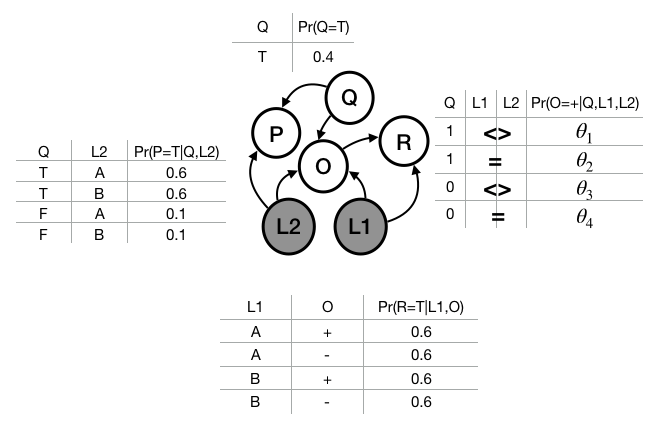
\includegraphics[width=\textwidth]{figs/BN.png}
  \end{minipage}\hfill
  \begin{minipage}[c]{0.45\textwidth}
    \caption{
        \small The model used for generating the datasets. There are four binary random variables, P, Q, O, and R. \textbf{P}: indicates whether or not the employee has high performance; \textbf{Q}: indicates whether or not an employee has high qualification; \textbf{O}: indicates whether or not the colleague submits the positive opinion towards the employee;  \textbf{R}: indicates whether or not the colleague has a positive opinion towards the employee;  \textbf{L1, L2}: indicates the label of the review provider and review receiver (observed).
    } \label{fig:BN}
  \end{minipage}
\end{figure}

We show the effectiveness of FairPSL by performing an empirical evaluation. We investigate two research questions in our experiments:
\begin{description}
\item[Q1] What is the effect of the fairness threshold $\delta$ on the fairness measures $RD/RC/RR$?
\item[Q2] How is decision quality affected by imposing $\delta$-fairness constraints?
\end{description}

Note that although we present the result for specific parameters of the framework in this section, we ran extensive analysis and the results we present are representative. We implemented the MAP inference routines of PSL and FairPSL in Python, using Gurobi-8.1\footnote{\url{www.gurobi.com}} as the backend solver. The FairPSL code, code for the data generator and data is publicly available\footnote{https://github.com/gfarnadi/FairPSL}. 

\subsection{Data generation}
  
We evaluate the FairPSL inference algorithm on synthetic datasets representing the performance review scenario (introduced in Example~\ref{ex:review}). The organization hierarchy is generated synthetically. 
The organization hierarchy generator is parameterized by two numbers: the number of employees in the organization ($n$) and the number of employees managed by each manager ($k$). Each employee is randomly assigned with a label \emph{A} or \emph{B}. An examples organization hierarchy with $n$=50 and $k$=3 is shown in Figure~\ref{fig:hierachy}.

\begin{figure}
  \begin{minipage}[c]{0.3\textwidth}
    \caption{
        \small An example of an organizational hierarchy with five levels and 50 employees with k=3. Each employee either has label A (shown with grey) or B (shown with white).
    }\label{fig:hierachy} 
	\end{minipage} \hfill
    \begin{minipage}[c]{0.7\textwidth}
    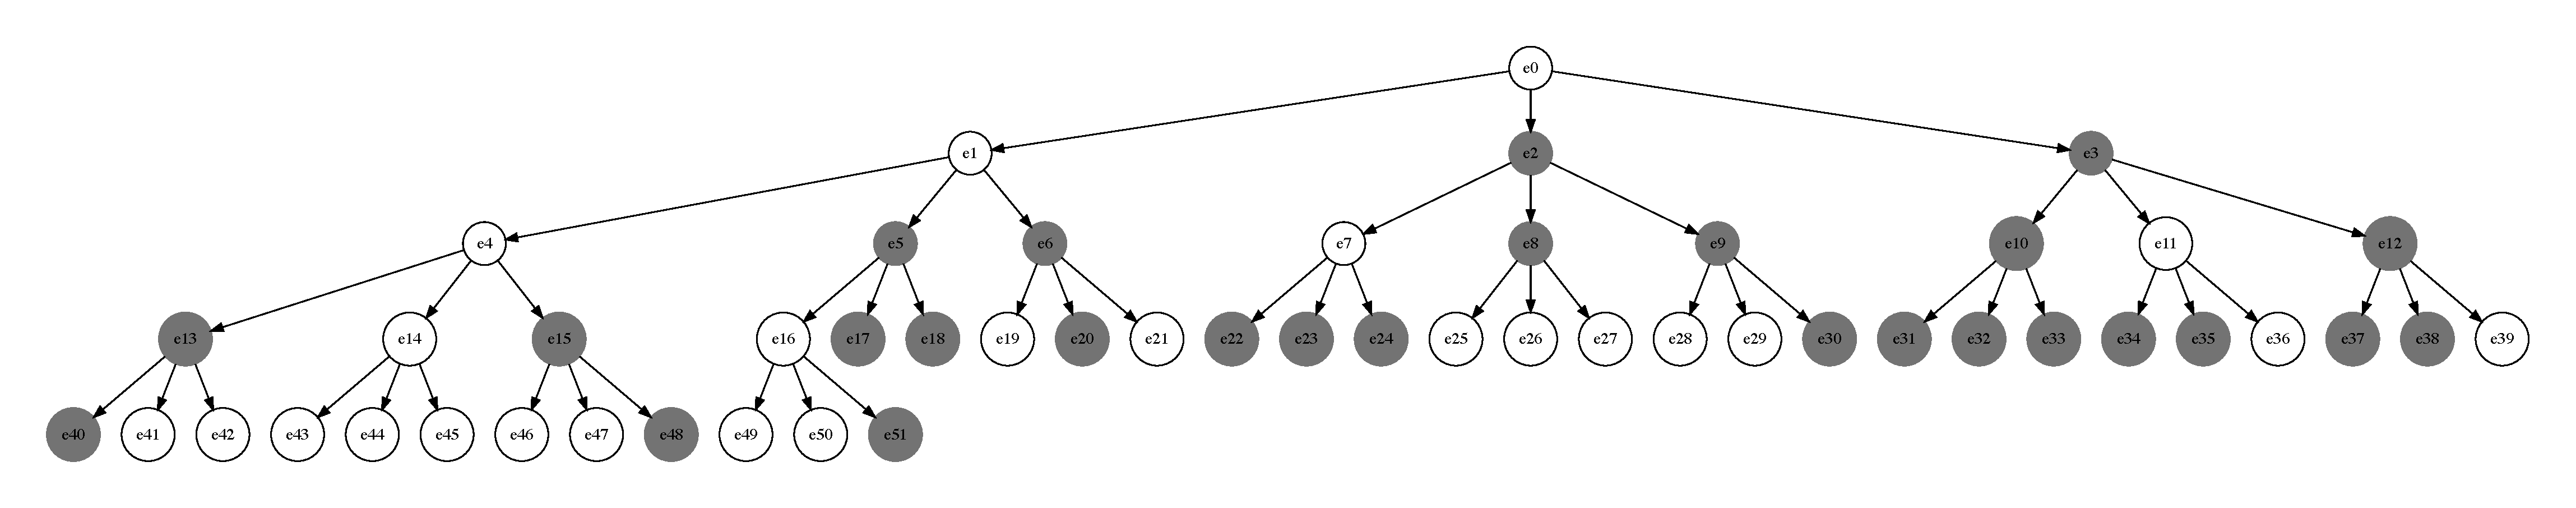
\includegraphics[width=\textwidth]{figs/Uni-hierachy.pdf}
  \end{minipage}
\end{figure}

For each employee, we use the generative model of Figure~\ref{fig:BN} to draw assignments for all the random variables. We assume that only $40\%$ of employees are qualified for promotion and regardless of their labels, employees submit only $60\%$ of their opinions. In addition, due to various personal and environmental factors, only $60\%$ of high quality employees perform well while $10\%$ of low quality employees also perform well regardless of their labels. Note that these numbers are not specific and just chosen for the framework to serve as a representative setting and a proof of concept. The conditional probability table for the opinion variable $O$ is parameterized by four values $(\theta_1, \theta_2, \theta_3, \theta_4)$ which together determine the degree of discrimination against the protected group. Since other parameters in the Bayesian network did not have a direct effect on the degree of discrimination, we fixed them to arbitrary values. 

The results presented in this section are based on an organization hierarchy  with $100$ employees where $k=5$. However, the results of the framework are not sensitive to the settings as we test the framework with various organization sizes ranging from $50$ to $500$ employees and various degree for $k$ ranging from $3$ to $10$. We generated seven datasets given the organization hierarchy using different values for the $\theta$ parameters: $(0.0,1.0,0.0,0.0)$, $(0.33,1.0,0.0,0.0)$, $(0.66,1.0,0.0,0.0)$, $(1.0,1.0,0.0,0.0)$, $(1.0,1.0,0.0,0.33)$, $(1.0,1.0,0.0,0.66)$, $(1.0,1.0,0.0,1.0)$. 
 
In the first three settings the discrimination originates from negative opinions towards qualified outgroup employees. The first setup is an extreme case where the opinion towards outgroup employees is always negative. The discrimination in the last three settings originates from positive opinions towards unqualified ingroup employees. The last setup is an extreme case where the opinion towards ingroup employees is always positive. The fourth setup represent unbiased opinions where employees are treated similarly based on their qualification. 

\paragraph{MAP Inference} We use the model presented in Table~\ref{tab:pslmodel} for MAP inference in PSL and FairPSL (recall that in FairPSL, the $\delta$-fairness constraints corresponding to one of the fairness measures are also added to the model). The observed atoms are $\textit{Manager(m,e)}$, $\textit{PositiveReview(e1,e2)}$ and labels of all employees. The truth values for all other atoms are obtained via MAP inference. We use the truth values obtained for the decision atoms $\textit{ToPromote(e)}$ to compute the fairness measures. We defined the discriminative pattern, and the protected and unprotected groups of this problem in Section~\ref{sec:formulation}.


\subsection{Evaluation results}

\begin{figure}
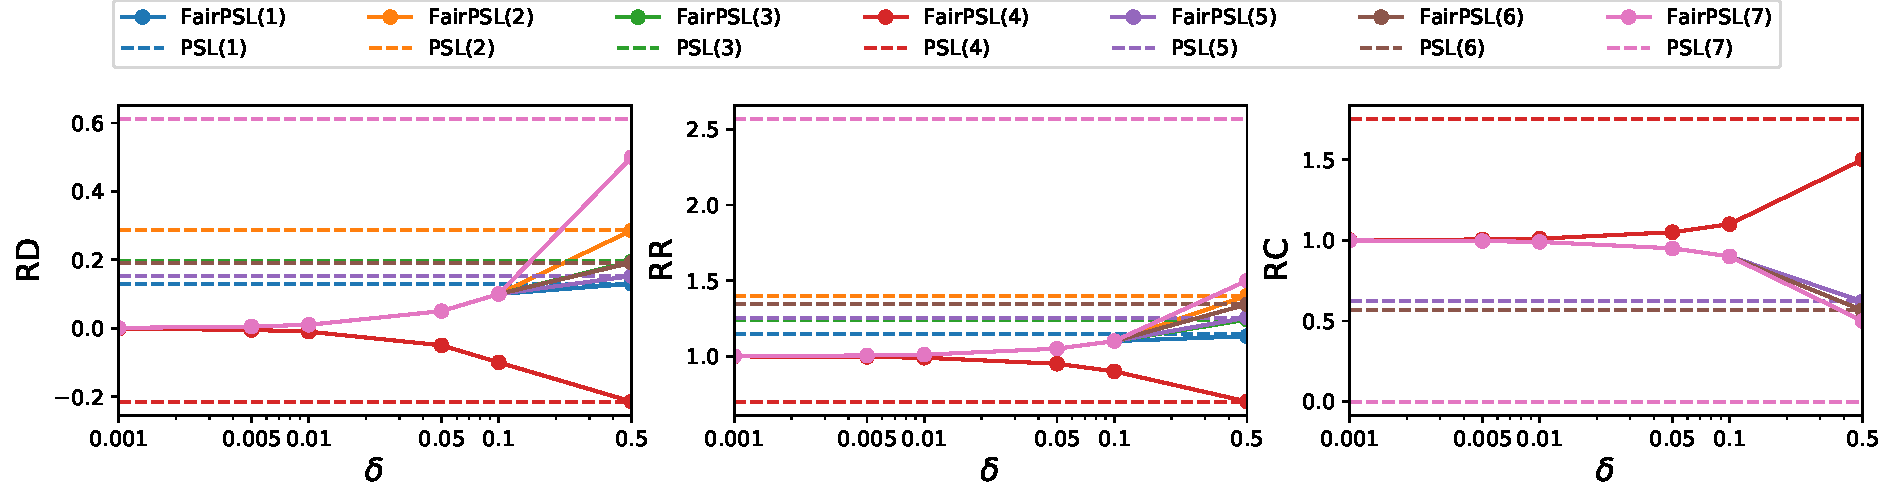
\includegraphics[width=1\linewidth]{figs/results_vis_uni_params.pdf}
\caption{\small Fairness score of predictions obtained by MAP inference of PSL and FairPSL, according to the fairness measures \emph{RD}, \emph{RR}, and \emph{RC}. The labels of datasets are mentioned with parenthesis next to the inference method. The FairPSL values of each measure are obtained by adding the $\delta$-fairness constraint of that measure.\label{fig:results}
}  
\end{figure}

To answer \textbf{Q1}, we run the MAP inference algorithm of PSL and FairPSL on seven synthetic datasets. 
We run the MAP inference of FairPSL multiple times on each dataset: For each of the three fairness measures, we add the corresponding $\delta$-fairness constraint with five thresholds $\{0.001, 0.005, 0.01, 0.05, 0.1, 0.5\}$.

Figure~\ref{fig:results} shows the fairness score of predictions in terms of the three fairness measures. As expected, tighter $\delta$-fairness constraints lead to better scores. Note that the best possible score according to RD is 0, as it computes a difference. Since RR and RC compute ratios, the best possible score according to these measures is 1. In our experiments, with any of these measures, taking $\delta = 0.001$ pushes the score of predictions to its limit.  

The $\delta$-fairness constraints modify the optimization problem of MAP inference by reducing the feasible region to solutions that conform with fairness guarantees. Research question \textbf{Q2} is concerned with the effect of this reduction on the accuracy of predictions. Note that decision quality is the same as the accuracy of predictions. To answer this question, we compare the inferred values for the decision atoms \textit{ToPromote(e)} against their actual values. These values are extracted from the known values of \textit{IsQualified(e)} according to rules 11 and 12 in Table~\ref{tab:pslmodel}. Figure~\ref{fig:accuracy} shows the area under the curve of the receiver operating characteristic~(AUC) of predicting the decision variable in three groups, namely the protected group, the unprotected group (i.e., promotion of the employees who have in-group managers), and all employees. By doing so, we make sure that our fairness constraints do not propagate bias towards either of the populations. Since the results of FairPSL with $\delta$-fairness constraints RR and RC are very similar to the results of RD, we only report the latter here.


\begin{figure}
    \centering
    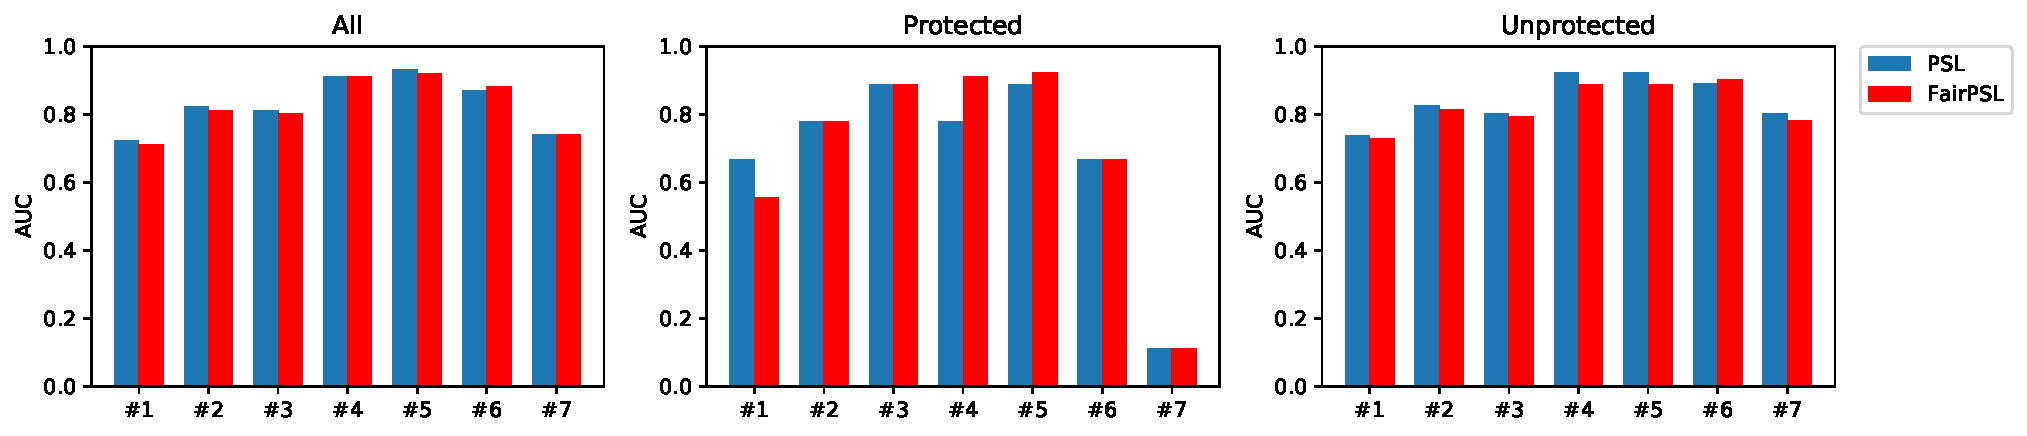
\includegraphics[width=\textwidth]{figs/roc.pdf}
    \caption{\small AUC score of predictions for truth values of unknown atoms \textit{ToPromote(e)} using MAP inference of PSL and FairPSL with $\delta$-fairness constraints $RD$ with $\delta=0.001$.}
    \label{fig:accuracy}
\end{figure}

According to Figure~\ref{fig:accuracy}, the results of both PSL and FairPSL in all seven datasets are close to each other. Note that although fairness may impose a cost in terms of overall accuracy, FairPSL often improves the accuracy of the protected class. Sometimes the overall predictions of FairPSL are even slightly better than PSL (e.g., dataset 6 and 7). As expected, the accuracy of the fourth setting where the opinions are unbiased are similar in both PSL and FairPSL. We observe that prediction of MAP inference for both FairPSL and PSL are similar, thus, in these settings at least, FairPSL guarantees fairness without hurting accuracy. Further investigation is required on the effect of the various ranges of discrimination (i.e., $\theta_1$, $\theta_2$, $\theta_3$, $\theta_4$) on the prediction results of FairPSL.



We also generate various types of organizations in which labels are not uniformly distributed, e.g., one population only occurs at the bottom levels of an organization. While we did not observe any differences in the behavior of our method with respect to accuracy and fairness measure, we found that the degree of discrimination is higher in such organizations. Further investigations on the structure of an organization on discrimination is an interesting direction for future research. 

\section{Conclusion and Future Directions}
\label{sec:conclusion}
Many applications of AI and machine learning affect peoples' lives in important ways. While there is a growing body of work on fairness in AI and ML, it assumes an individualistic notion of fairness.   In this paper, we have proposed a general framework for relational fairness which includes both a rich language for defining discrimination patterns and an efficient algorithm for performing inference subject to fairness constraints. We show our approach enforces fairness guarantees while preserving the accuracy of the predictions. 

There are many avenues for expanding on this work. For example, here we assumed that the discriminative pattern is given, however an automatic mechanism to extract discriminatory situations hidden in a large amount of decision records is an important and required task. Discrimination discovery has been studied for attribute-based fairness~\cite{pedreschi2013discovery}. An interesting next step is discrimination pattern discovery in relational data.

\section*{Acknowledgements}
This work is supported by the National Science Foundation under Grant Numbers CCF-1740850 and IIS-1703331. Golnoosh Farnadi and Behrouz Babaki are  supported by postdoctoral scholarships from IVADO through the Canada First Research Excellence Fund (CFREF) grant.

\begin{thebibliography}{10}
\itemsep=1pt 
\begin{small}

\bibitem{EUlaw}
European union legislation. (a) racial equality directive, 2000; (b) employment
  equality directive, 2000; (c) gender employment directive, 2006; (d) equal
  treatment directive (proposal), 2008.

\bibitem{UKlaw}
{UK} legislation. (a) sex discrimination act, 1975, (b) race relation act,
  1976.

\bibitem{USlaw}
United nations legislation. (a) universal declaration of human rights, 1948,
  (c) convention on the elimination of all forms of racial discrimination,
  1966, (d) convention on the elimination of all forms of discrimination
  against women, 1979.

\bibitem{alshukaili:iswc16}
Duhai Alshukaili, Alvaro A.~A. Fernandes, and Norman~W. Paton.
\newblock Structuring linked data search results using probabilistic soft
  logic.
\newblock In {\em International Semantic Web Conference {(1)}}, volume 9981 of
  {\em Lecture Notes in Computer Science}, pages 3--19, 2016.

\bibitem{bach:jmlr17}
Stephen~H. Bach, Matthias Broecheler, Bert Huang, and Lise Getoor.
\newblock Hinge-loss markov random fields and probabilistic soft logic.
\newblock {\em Journal of Machine Learning Research}, 18:109:1--109:67, 2017.

\bibitem{barocas2016big2}
Solon Barocas and Andrew~D Selbst.
\newblock Big data's disparate impact.
\newblock {\em California Law Review}, 104:671, 2016.

\bibitem{boyd2014networked}
Danah Boyd, Karen Levy, and Alice Marwick.
\newblock The networked nature of algorithmic discrimination.
\newblock In {\em Data and discrimination: Collected essays}, pages 53--57.
  2014.

\bibitem{brewer1979group}
Marilynn~B Brewer.
\newblock In-group bias in the minimal intergroup situation: A
  cognitive-motivational analysis.
\newblock {\em Psychological bulletin}, 86(2):307, 1979.

\bibitem{brewer2007social}
Marilynn~B Brewer.
\newblock The social psychology of intergroup relations: Social categorization,
  ingroup bias, and outgroup prejudice.
\newblock {\em Social Psychology: Handbook of Basic Principles}, 2007.

\bibitem{chouldechova2017fair2}
Alexandra Chouldechova.
\newblock Fair prediction with disparate impact: {A} study of bias in
  recidivism prediction instruments.
\newblock {\em CoRR}, abs/1703.00056, 2017.

\bibitem{dwork2012fairness3}
Cynthia Dwork, Moritz Hardt, Toniann Pitassi, Omer Reingold, and Richard~S.
  Zemel.
\newblock Fairness through awareness.
\newblock In {\em {ITCS}}, pages 214--226. {ACM}, 2012.

\bibitem{ebrahimi:emnlp16}
Javid Ebrahimi, Dejing Dou, and Daniel Lowd.
\newblock Weakly supervised tweet stance classification by relational
  bootstrapping.
\newblock In {\em {EMNLP}}, pages 1012--1017. The Association for Computational
  Linguistics, 2016.

\bibitem{farnadi2018fairness}
Golnoosh Farnadi, Behrouz Babaki, and Lise Getoor.
\newblock Fairness in relational domains.
\newblock In {\em AAAI/ACM Conference on AI, Ethics, and Society (AIES)}, pages
  108--114. ACM, 2018.

\bibitem{feldman2015certifying2}
Michael Feldman, Sorelle~A. Friedler, John Moeller, Carlos Scheidegger, and
  Suresh Venkatasubramanian.
\newblock Certifying and removing disparate impact.
\newblock In {\em {KDD}}, pages 259--268. {ACM}, 2015.

\bibitem{getoor2007introduction}
Lise Getoor and Ben Taskar.
\newblock {\em {Introduction to Statistical Relational Learning}}.
\newblock MIT press Cambridge, 2007.

\bibitem{hardt2016equality3}
Moritz Hardt, Eric Price, and Nati Srebro.
\newblock Equality of opportunity in supervised learning.
\newblock In {\em {NIPS}}, pages 3315--3323, 2016.

\bibitem{kamishima2011fairness}
Toshihiro Kamishima, Shotaro Akaho, and Jun Sakuma.
\newblock Fairness-aware learning through regularization approach.
\newblock In {\em ICDMW}, pages 643--650. {IEEE} Computer Society, 2011.

\bibitem{kouki:recsys15}
Pigi Kouki, Shobeir Fakhraei, James~R. Foulds, Magdalini Eirinaki, and Lise
  Getoor.
\newblock Hyper: {A} flexible and extensible probabilistic framework for hybrid
  recommender systems.
\newblock In {\em RecSys}, pages 99--106. {ACM}, 2015.

\bibitem{counterfactualfairness}
Matt~J. Kusner, Joshua~R. Loftus, Chris Russell, and Ricardo Silva.
\newblock Counterfactual fairness.
\newblock In {\em {NIPS}}, pages 4069--4079, 2017.

\bibitem{Pedreschi:2012}
Dino Pedreschi, Salvatore Ruggieri, and Franco Turini.
\newblock A study of top-k measures for discrimination discovery.
\newblock In {\em {SAC}}, pages 126--131. {ACM}, 2012.

\bibitem{pedreschi2013discovery}
Dino Pedreschi, Salvatore Ruggieri, and Franco Turini.
\newblock The discovery of discrimination.
\newblock In {\em Discrimination and Privacy in the Information Society},
  volume~3 of {\em Studies in Applied Philosophy, Epistemology and Rational
  Ethics}, pages 91--108. Springer, 2013.

\bibitem{ridgeway2004unpacking}
Cecilia~L Ridgeway and Shelley~J Correll.
\newblock Unpacking the gender system: A theoretical perspective on gender
  beliefs and social relations.
\newblock {\em Gender \& society}, 18(4):510--531, 2004.

\bibitem{sridhar:bioinformatics16}
Dhanya Sridhar, Shobeir Fakhraei, and Lise Getoor.
\newblock A probabilistic approach for collective similarity-based drug-drug
  interaction prediction.
\newblock {\em Bioinformatics}, 32(20):3175--3182, 2016.

\bibitem{verma2018fairness2}
Sahil Verma and Julia Rubin.
\newblock Fairness definitions explained.
\newblock In {\em 2018 IEEE/ACM International Workshop on Software Fairness
  (FairWare)}, pages 1--7. IEEE, 2018.

\bibitem{west2014exploiting}
Robert West, Hristo~S. Paskov, Jure Leskovec, and Christopher Potts.
\newblock Exploiting social network structure for person-to-person sentiment
  analysis.
\newblock {\em {TACL}}, 2:297--310, 2014.

\bibitem{zafar2017parity}
Muhammad~Bilal Zafar, Isabel Valera, Manuel Gomez{-}Rodriguez, Krishna~P.
  Gummadi, and Adrian Weller.
\newblock From parity to preference-based notions of fairness in
  classification.
\newblock In {\em {NIPS}}, pages 228--238, 2017.

\bibitem{zemel2013learning}
Richard~S. Zemel, Yu~Wu, Kevin Swersky, Toniann Pitassi, and Cynthia Dwork.
\newblock Learning fair representations.
\newblock In {\em {ICML} {(3)}}, volume~28 of {\em {JMLR} Workshop and
  Conference Proceedings}, pages 325--333. JMLR.org, 2013.

\end{small}
\end{thebibliography}

\end{document}

\end{article}


\begin{article}
{doppioDB 1.0: Machine Learning inside a Relational Engine}
{Gustavo Alonso, Zsolt Istvan, Kaan Kara, Muhsen Owaida, David Sidler}
\graphicspath{{submissions/gustavo/}}
%\documentclass[11pt,dvipdfm]{article}
\documentclass[11pt]{article}
\usepackage{deauthor,times,graphicx} %required
\usepackage{amsmath,amssymb}
\usepackage{multirow}
\usepackage{algorithm}
\usepackage{algpseudocode}
\usepackage{todonotes}
\usepackage{url}

% \graphicspath{{farnadi/}}

\newtheorem{mydef}{\textbf{Definition}}
\newtheorem{myex}{\textbf{Example}}
\newtheorem{mytheorem}{\textbf{Theorem}}


\begin{document}

\title{A Declarative Approach to Fairness in Relational Domains}
\author{Golnoosh Farnadi$^{1,2}$, Behrouz Babaki$^1$, Lise Getoor$^3$\\
$^1$Polytechnique Montr\'{e}al, $^2$ Mila, $^3$ UC Santa Cruz \\
farnadig@mila.quebec, behrouz.babaki@polymtl.ca, getoor@soe.ucsc.edu}

\maketitle

\begin{abstract}
AI and machine learning tools are being used with increasing frequency for decision making in domains that affect peoples' lives such as employment, education, policing and %loan approval
financial qualifications. These uses raise concerns about biases of algorithmic discrimination and have motivated the development of fairness-aware machine learning. However, existing fairness approaches are based solely on attributes of individuals. In many cases, discrimination is much more complex, and taking into account the social, organizational, and other connections between individuals is important. We introduce new notions of fairness that are able to capture the relational structure in a domain. We use first-order logic to provide a flexible and expressive language for specifying complex relational patterns of discrimination. Furthermore, we extend an existing statistical relational learning framework, probabilistic soft logic~(PSL), to incorporate our definition of relational fairness. We refer to this fairness-aware framework FairPSL. FairPSL makes use of the logical definitions of fairnesss but also supports a probabilistic interpretation. In particular, we show how to perform maximum a posteriori~(MAP) inference by exploiting probabilistic dependencies within the domain while avoiding violations of fairness guarantees. Preliminary empirical evaluation shows that we are able to make both accurate and fair decisions.
\end{abstract}

\section{Introduction}
\label{sec:introduction}

Over the past few years, AI and machine learning have become essential components in operations that drive the modern society, e.g., in financial, administrative, and educational spheres. \emph{Discrimination} happens when qualities of individuals which are not relevant to the decision making process influence the decision. Delegating decision making to an automated process raises questions about discriminating against individuals with certain traits based on biases in the data. This is especially important when the decisions have the potential to impact the lives of individuals, for example, the decisions on granting loans, assigning credit, and employment. 

\emph{Fairness} is defined as the absence of discrimination in a decision making process. The goal of \emph{fairness-aware} machine learning is to ensure that the decisions made by an algorithm do not discriminate against a population of individuals~\cite{feldman2015certifying2,boyd2014networked,hardt2016equality3}. Fairness has been well studied in the social sciences and legal scholarship (for an in-depth review see~\cite{barocas2016big2}), and there is emerging work on fairness-aware ML within the AI and computer science communities. For example, fairness through awareness/Lipschitz property~\cite{dwork2012fairness3}, individual fairness~\cite{zemel2013learning}, statistical parity/group fairness~\cite{kamishima2011fairness}, counterfactual fairness~\cite{counterfactualfairness}, demographic parity/disparate impact~\cite{feldman2015certifying2,chouldechova2017fair2}, preference-based fairness~\cite{zafar2017parity}, and equality of opportunity~\cite{hardt2016equality3}.

The existing work in fairness-aware machine learning is based on a definition of discrimination where a decision is influenced by an \emph{attribute} of an individual. An attribute value upon which discrimination is based (such as gender, race, or religion) is called a \emph{sensitive attribute}. The sensitive attribute defines a population of vulnerable individuals known as the \emph{protected group}. A fair decision-making process treats the protected group the same as the \emph{unprotected group}. 

However, in many social contexts, discrimination is the result of complex interactions and can not be described solely in terms of attributes of an individual. For example, consider an imaginary scenario in an organization in which younger female workers who have older male supervisors have lower chances of promotion than their male counterparts.\footnote{Of course, many other patterns may be possible: female bosses may promote female subordinates and discriminate against male workers, or male bosses may promote female employees.  Our goal is to provide a general framework which is able to describe arbitrarily complex discrimination patterns.} 
 This discrimination pattern involves two attributes of the individual (gender and age), a relationship with another individual (supervisor), and two attributes of the second individual. Addressing such complex cases poses two challenges. First, the concepts of discrimination and fairness need to be extended to capture not only attributes of individuals but also the relationships between them. Second, a process is required that ensures that fair decisions are made about individuals who are affected by such patterns. In this paper we address both of these challenges.
We use first-order logic (FOL) to extend the notion of fairness to the relational setting. FOL is an expressive representation for relational problems which is also widely used for learning in relational domains. Moreover, we extend an existing framework for statistical relational learning~\cite{getoor2007introduction} called probabilistic soft logic (PSL)\footnote{http://psl.linqs.org/}~\cite{bach:jmlr17}. PSL combines logic and probability for learning and reasoning over uncertain relational domains. One of the most common reasoning tasks in PSL is called maximum a posteriori (MAP) inference, which is performed by finding the most probable truth values for unknowns over a set of given evidence. We develop a new MAP inference algorithm which is able to maximize the a posteriori values of unknown variables \emph{subject to} fairness guarantees. An early version of this paper which this work builds upon and extends appeared in~\cite{farnadi2018fairness}.

\looseness-1
Our contributions are as follows: 1) we propose fairness-aware machine learning for the relational setting; 2) we extend PSL into a fairness-aware framework called FairPSL which can represent the logical definition of fairness; 3) we develop a new MAP inference algorithm which is able to maximize the posteriori values of unknown variables \emph{subject to} fairness guarantees; 4) we empirically evaluate our proposed framework on synthetic data. 

\section{Motivation}
\label{sec:motivation}

Discrimination in social contexts have been studied in the field of social psychology~\cite{brewer2007social,brewer1979group,ridgeway2004unpacking}. There is a large literature on various aspects of relational bias in social contexts such as \emph{in-group-out-group bias}, \emph{gender bias}, and \emph{ethnicity-based favoritism} that can result in discrimination. 
As an example, consider gender bias in the workplace that reflects stereotypically masculine criteria and male-based favoritism. Such gender bias 
typically places women in lower positions and negatively impacts their opportunities. Further, lack of women in leadership positions may affect the promotion of women and results in a glass ceiling that keeps women from rising beyond a certain level in the hierarchy. This scenario shows that considering  protected attributes such as gender is not always sufficient to detect the source of bias and avoid discrimination, one also has to consider the relational information, in this case the organization hierarchy. Note that this can be generalized to any ingroup/outgroup scenario where the sensitive attribute could be race, religion, age, marital-status, etc.

The existing work on designing fair algorithms in machine learning exclusively focuses on \emph{attribute-based fairness}, which is based on the following assumptions: First, there is an assumption that the individuals (sometimes referred to as units or entities) are independent and described by simple attribute vectors. Second, the group for which one wishes to ensure fairness (known as the \emph{protected group}) is defined on the basis of some attribute values. Finally, there is a decision that is associated with each individual, and the goal is to ensure that members of the protected group are subject to a fair decision (we discuss different fairness measures in Section~\ref{sec:fairnessmeasure}).  We illustrate  attribute-based fairness in the following example. 

\begin{myex}[Loan Processing]
\label{ex:loan}
A bank bases its decisions about granting a loan on attributes of the applicant. The goal is to decide whether to grant a loan to an applicant using a predictive model. The bank needs to ensure that the obey fair lending practices and ensure that gender, race, sexual orientation of applicants has no influence on the decision. In this scenario, the protected group is the historically disadvantaged applicants.  
\end{myex}
The current fairness-aware machine learning techniques are not capable of modeling relations and hence cannot be used to make the decision making model fair. However, in many decision making scenarios, especially in social and organizational settings, the domain is relational, and the protected group itself might be best represented using a relational definition. We illustrate this setting in the following scenario:
\begin{myex}[Performance Review]
\label{ex:review}
Consider an organization where decisions about the promotion of employees is based on two criteria: 1) an objective performance measure, and 2) the opinion of their direct and indirect managers above them. The opinions are inferred from the performance reviews which are collected periodically. Not every manager can submit a review for all its subordinates, this is especially the case for top-level managers who have a large number of subordinates. Hence, the opinions of managers are collectively inferred from the opinions of their sub-ordinates. However, some employees may be biased, and judge other employees unfavorably, by favoring employees who are similar to themselves (same gender, race, religion, etc.) over employees who are dissimilar. The organization needs to ensure that promotion of employees do not have any relational bias caused by in-group-out-group favoritism.

\end{myex}
Example~\ref{ex:review} describes a prediction problem over a database that consists of relations between employees. Such prediction tasks are best handled by techniques from the relational learning domain. To ensure fair prediction in such settings, we need to extend the notion of \emph{attribute-based fairness} to \emph{relational fairness}. Throughout this paper, we use the performance review problem as a running example for relational fairness.

\section{Fairness Formalism}
\label{sec:formulation}

A representation that can describe different types of entities and different relationships between them is called relational. In this section, we use first-order logic to define relational fairness. We employ first-order logic as an expressive representation formalism which can represent objects and complex relationships between them. We start by defining an atom:

\begin{mydef}[Atom]
An atom is an expression of the form $P(a_1, a_2, \ldots, a_n)$ where each argument $a_1, a_2,$ $\ldots,$ $a_n$ is either a constant or a variable. The finite set of all possible substitutions of a variable to a constant for a particular variable $a$ is called its \textit{domain} $D_{a}$. If all variables in $P(a_1, a_2, \ldots, a_n)$ are substituted by some constant from their respective domain, then we call the resulting atom a \textit{ground atom}. 
\end{mydef}

\begin{myex}
In our loan processing problem (Example~\ref{ex:loan}), we can represent applicants' attributes by atoms. For instance, atom $Female(v)$ indicates whether or not applicant $v$ is female. Similarly, we can represent relations with atoms. In the performance review problem in Example~\ref{ex:review} the atom $Manager(m,e)$ indicates whether or not employee $m$ is a direct or indirect manager of employee $e$.
\end{myex}

The relational setting provides the flexibility to express complex definitions with formulae.

\begin{mydef}[Formula] 
A formula is defined by induction: every atom is a formula. If $\alpha$ and $\beta$ are formulae, then $\alpha \vee \beta$, $\alpha \wedge \beta$, $\neg \alpha$, $\alpha \rightarrow \beta$ are formulae. If $x$ is a variable and $\alpha$ is a formula, then the quantified expressions of the form $\exists x$ $\alpha$ and $\forall x$ $\alpha$ are formulae.    
\end{mydef}

To characterize groups of individuals based on a formula, we define the notion of \emph{population}.

\begin{mydef}[Population]
We denote formula $F$ which has only one free variable $v$ (i.e., other variables in $F$ are quantified) by $F[v]$. The population defined by $F[v]$ is the set of substitutions of $v$ for which $F[v]$ holds.   
\end{mydef}


\begin{myex}
\label{ex:disformula}
Consider the formula $F[v] := \forall u, \, \textit{Manager}(u,v) \rightarrow \neg \textit{SameGroup}(u, v)$. The population specified by this formula is the set of individuals all of whose managers belong to a group different from theirs. 
\end{myex}

The truth value of a formula is derived from the truth value of atoms that it comprises, according to the rules of logic. Each possible assignment of truth values to ground atoms is called an \emph{interpretation}. 


\begin{mydef}[Interpretation]
An interpretation $I$ is a mapping that associates a truth value $I(P)$ to each ground atom $P$. For Boolean truth values, $I$ associates true to 1 and false to 0 truth values. For soft logic (see Definition~\ref{def:softlogic}) $I$ maps each ground atom $P$ to a truth value in interval $[0, 1]$.
\end{mydef}

In attribute-based fairness, it is assumed that there is a certain attribute of individuals, i.e, the sensitive attribute,  that we do not want to affect a decision. Gender, race, religion and marital status are examples of sensitive attributes. Discrimination has been defined in social science studies as a treatment in favor or against a group of individuals given their sensitive attribute. This group of individuals is the protected group. 

In a relational setting, both the sensitive attributes of an individual and their participation in various relations may have an undesired effect on the final decision. We characterize the protected group in a relational setting by means of a population. In practice, we are often interested in maintaining fairness for a specific population such as applicants, students, employees, etc. This population is then partitioned into the protected and unprotected groups. We define a \emph{discriminative pattern} which is a pair of formulae to capture these groups: 1) $F_1[v]$: to specify the difference between the protected and unprotected groups and 2) $F_2[v]$: to specify the population over which we want to maintain fairness. 

\begin{mydef}[Discriminative pattern]
A discriminative pattern is a pair $\textit{DP}[v]:=(F_1[v], F_2[v])$ , where $F_1[v]$ and $F_2[v]$ are formulae.
\end{mydef}

\begin{myex}
\label{ex:pattern}
The two formulae in the discrimination pattern $\textit{DP}[v]:= \big((\forall u, \,  \textit{Manager}(u,v) \rightarrow  \neg \textit{SameGroup}(u, v)),$ $\textit{Employee}(v)\big)$ specify two populations, namely all employees and those employees who belong to a group different from their managers.
\end{myex}

Given the definition of the discriminative pattern, we have a rich language to define the scope of the protected and unprotected groups in a relational setting.

\begin{mydef}[Protected group] Given an interpretation $I$, the protected group is a population of the form:
{$$PG :=\{ v : F_1[v] \wedge F_2[v]\}$$}
which is defined as the set of all instances hold for variable $v$ for which $F_1[v] \wedge F_2[v]$ is true under interpretation $I$, that is, $I(F_1[v] \wedge F_2[v]) = 1$. 
Similarly, the \emph{unprotected group} is a population of the form: 
{$$UG := \{ v : \neg F_1[v] \wedge  F_2[v]\}$$}
which is defined as the set of all instances hold for variable $v$ 
for which $I(\neg F_1[v] \wedge F_2[v]) = 1$. 
\end{mydef}

\begin{myex}
The protected group of the discrimination pattern specified in Example~\ref{ex:pattern} is {$PG := \big\{ v : \big(\forall u, \,$ $ \textit{Manager}(u, v) \rightarrow \neg \textit{SameGroup}(u, v)\big) \wedge \textit{Employee}(v) \big\}$} and the unprotected group is {$UG :=  \big\{ v:  \big(\exists u, \, \textit{Manager}(u,v) \wedge \textit{SameGroup}(u, v)\big) \wedge \textit{Employee}(v) \big\}$}. This means our protected group is the set of employees belonging to a group different from their managers,
and our unprotected group consists of other employees. 
\end{myex}

Discrimination is defined in terms of a treatment or decision that distinguishes between the protected and unprotected groups. Here we define the \emph{decision} atom.
\begin{mydef}[Decision atom] A decision atom $d(v)$ is an atom containing exactly one variable $v$ that specifies a decision affecting the protected group which is defined either by law or end-user.
\end{mydef}
\begin{myex}
The decision atom ${\textit ToPromote}(v)$ indicates whether or not $v$ receives a promotion.
\end{myex}

Note that the fairness formulation in this section is designed for the relational setting, however relational fairness subsumes the attribute-based fairness such that: a sensitive attribute is defined by an atom with one argument and $F_2[v]$ in discrimination pattern is $\textit{Applicant}(v)$. For example, discrimination pattern of our loan processing problem in Example~\ref{ex:loan} is of the form $\textit{DP} := ( \textit{Female}(v), \textit{Applicant}(v))$ that denotes female applicants as the protected group (i.e., $PG :=  \{ v: \textit{Female}(v) \}$) and male applicants as the unprotected group (i.e., $UG := \{ v: \neg \textit{Female}(v)\}$).


\section{Fairness Measures}
\label{sec:fairnessmeasure}

Over the past few years, many fairness measures have been introduced~\cite{verma2018fairness2}. An important class of these measures are \emph{group fairness} measures which quantify the inequality between different subgroups. Some of the most popular measures in this class include \emph{equal opportunity}, \emph{equalized odds}, and \emph{demographic parity}~\cite{hardt2016equality3}. In this paper we restrict our focus to the latter. In an attribute-value setting, demographic parity means that the decision should be independent of the protected attributes. Assume that binary variables $A$ and $C$ denote the decision and protected attributes, and the preferred value of $A$ is one. Demographic parity requires that:

\begin{equation*}
    P(A=1 | C=0) = P(A=1 | C=1)
\end{equation*}

We will now generalize this measure to the relational setting using the notations defined in Section~\ref{sec:formulation}. Let $a$ and $c$ denote the counts of denial (i.e., negative decisions) for protected and unprotected groups, and $n_{1}$ and $n_{2}$ denote their sizes, respectively. Given the decision atom $d(v)$, discriminative pattern $\textit{DP}(F_1[v], F_2[v])$, and interpretation $I$, these counts are computed by the following equations: 
{
\begin{flalign}
    & a \equiv \sum_{v \in D_v} I\big( \neg d(v) \wedge  F_1[v] \wedge F_2[v]) \label{eq:a}\\
    & c \equiv \sum_{v \in D_v} I\big( \neg d(v) \wedge  \neg F_1[v] \wedge  F_2[v]) \label{eq:c}\\
    & n_{1} \equiv \sum_{v \in D_v} I\big(F_1[v] \wedge F_2[v]) \label{eq:n1}\\
    & n_{2} \equiv \sum_{v \in D_v} I\big(\neg F_1[v] \wedge  F_2[v]) \label{eq:n2}
\end{flalign}}
The proportions of denying for protected and unprotected groups are $p_1 = \frac{a}{n_1}$ and $p_2 = \frac{c}{n_2}$, respectively. There are a number of data-driven measures~\cite{Pedreschi:2012} which quantify demographic disparity and can be defined in terms of $p_1$ and $p_2$:
\begin{itemize}
    \item \textbf{Risk difference}: $RD = p_1 - p_2$, also known as absolute risk reduction. 
    \item \textbf{Risk Ratio}: $RR = \frac{p_1}{p_2}$, also known as relative risk. 
    \item \textbf{Relative Chance}: $RC = \frac{1 - p_1}{1 - p_2}$ also, known as selection rate.
\end{itemize}
These measures have been used in the legal systems of European Union, UK, and US~\cite{EUlaw,UKlaw,USlaw}. Notice that RR is the ratio of the proportion of benefit denial between the protected and unprotected groups, while RC is the ratio of the proportion of benefit granted. Finally, we introduce the notion of $\delta$-fairness.

\begin{mydef}[$\delta$-fairness]
If a fairness measure for a decision making process falls within some $\delta$-window, then the process is \emph{$\delta\text{-fair}$}. Given $0 \leq \delta \leq 1$, the  $\delta$-windows for measures RD/RR/RC are defined as:
{\begin{flalign*}
	     - \delta \leq &RD \leq \delta \\
	     1- \delta \leq &RR \leq 1+ \delta\\
	     1- \delta \leq &RC \leq 1+ \delta
	\end{flalign*}}
\end{mydef}

To overcome the limitations of attribute-based fairness, we introduce a new statistical relational learning~(SRL) framework~\cite{getoor2007introduction} suitable for modelling fairness in relational domain. In the next section, we review probabilistic soft logic~(PSL). We then extend PSL with the definition of relational fairness introduced above in Section~\ref{sec:fairMAP}. Our fairness-aware framework, ``FairPSL'', is the first SRL framework that performs fair inference. 

\section{Background: Probabilistic Soft Logic}
\label{sec:psl}

In this section, we review the syntax and semantics of PSL, and in the next section we extend MAP inference in PSL with fairness constraints to define MAP inference in FairPSL.

PSL is a probabilistic programming language for defining hinge-loss Markov random fields~\cite{bach:jmlr17}. Unlike other SRL frameworks whose atoms are Boolean, atoms in PSL can take continuous values in the interval $[0,1]$. PSL is an expressive modeling language that can incorporate domain knowledge with first-order logical rules and has been used successfully in various domains, including bioinformatics~\cite{sridhar:bioinformatics16}, recommender systems~\cite{kouki:recsys15}, natural language processing~\cite{ebrahimi:emnlp16}, information retrieval~\cite{alshukaili:iswc16}, and social network analysis~\cite{west2014exploiting}, among many others. 
 
A PSL model is defined by a set of first-order logical rules called \emph{PSL rules}.

\begin{mydef} [PSL rule] a PSL rule $r$ is an expression of the form:
{\begin{equation}
\lambda_{r}: T_1 \land T_2 \land \ldots \land T_w \rightarrow H_1 \vee H_2 \vee \ldots \vee H_l
\end{equation}}

where { $T_1, T_2, \ldots, T_w, H_1, H_2, \ldots, H_l$} are atoms or negated atoms and { $\lambda_{r} \in \mathbb{R}^{+} \cup \infty$} is the weight of the rule $r$.  We call { $T_1 \land T_2 \land \ldots \land T_w$} the body of $r$ ($r_{body}$), and { $H_1 \vee H_2 \vee \ldots \vee H_l$} the head of $r$ ($r_{head}$).
\end{mydef}


Since atoms in PSL take on continuous values in the unit interval $[0,1]$, next we define soft logic to calculate the value of the PSL rules under an interpretation $I$.

\begin{mydef}[Soft logic]
\label{def:softlogic}
The ({$\tilde{\wedge}$}) and ({$\tilde{\vee}$}) and negation ({$\tilde{\neg}$}) are defined as follows. For {$m, n \in [0,1]$} we have: {$m \tilde{\wedge} n = \max(m+n -1, 0)$}, {$m \tilde{\vee} n = \min(m+n , 1)$} and {$\tilde{\neg} m = 1 - m$}. The $\, \tilde{} \,$ indicates the relaxation over Boolean values.
\end{mydef}

The probability of truth value assignments in PSL is determined by the rules' \emph{distance to satisfaction}.

\begin{mydef}[The distance to satisfaction]
The distance to satisfaction $d_{r}(I)$ of a rule $r$ under an interpretation $I$ is defined as:
{
\begin{equation}
d_{r}(I) = \max\{0, I(r_{body})-I(r_{head})\}
\end{equation}}
\end{mydef}

By using Definition~\ref{def:softlogic}, one can show that the closer the interpretation of a grounded rule $r$ is to 1, the smaller its distance to satisfaction. A PSL model induces a distribution over interpretations $I$. Let $R$ be the set of all grounded rules, then the probability density function is:
{
\begin{equation}
f(I) ={\frac{1}{Z}} \exp[-\sum_{r\in R} \lambda_{r}(d_{r}(I))^p]
\label{eq:potential}
\end{equation}
}
\noindent where { $\lambda_{r}$} is the weight of rule $r$, {
$Z = \int_{I} \exp[ -\sum_{r\in R} \lambda_{r}(d_{r}(I))^p]$
} is a normalization constant, and { $p \in \{1,2\}$} provides a choice of two different loss functions, $p=1$ (i.e., linear), and $p=2$ (i.e, quadratic). These probabilistic models are instances of hinge-loss Markov random fields~(HL-MRF)~\cite{bach:jmlr17}. The goal of maximum a posteriori (MAP) inference is to find the most probable truth assignments $I_{\textit{MPE}}$ of unknown ground atoms given the evidence which is defined by the interpretation $I$. Let $X$ be all the evidence, i.e., $X$ is the set of ground atoms such that $\forall x \in X, I(x)$ is known, and let $Y$ be the set of ground atoms such that $\forall y \in Y, I(y)$ is unknown. Then we have
{
\begin{equation}
I_{\textit{MAP}}(Y) = \textit{arg}\max_{I(Y)} P(I(Y)|I(X))
\end{equation}}
Maximizing the density function in Equation~\ref{eq:potential} is equivalent to minimizing the weighted sum of the distances to satisfaction of all rules in PSL. 

\begin{table*}[t]
    \centering
    \begin{tabular}{|lll|}
    \hline
    &&\\
    $R1$ & $\lambda_1$ &: $\textit{IsQualified}(e) \rightarrow \textit{HighPerformance}(e)$ \\
    $R2$ & $\lambda_1$ &: $\neg \textit{IsQualified}(e) \rightarrow \neg \textit{HighPerformance}(e)$ \\
    $R3$ & $\infty$ &: $\textit{PositiveReview}(e1, e2) \rightarrow \textit{PositiveOpinion}(e1, e2)$ \\
    $R4$ & $\infty$ &: $\neg \textit{PositiveReview}(e1, e2) \rightarrow \neg \textit{PositiveOpinion}(e1, e2)$ \\
    $R5$ & $\lambda_1$ &: $\textit{PositiveOpinion}(e1, e2) \wedge \textit{Manager}(m, e1) \rightarrow \textit{PositiveOpinion}(m, e2)$ \\
    $R6$ & $\lambda_1$ &: $\neg \textit{PositiveOpinion}(e1, e2) \wedge \textit{Manager}(m, e1) \rightarrow \neg \textit{PositiveOpinion}(m, e2)$ \\
    $R7$ & $\lambda_1$ &: $\textit{PositiveOpinion}(m, e) \wedge \textit{Manager}(m, e) \rightarrow \textit{IsQualified}(e)$ \\
    $R8$ & $\lambda_1$ &: $\neg \textit{PositiveOpinion}(m, e) \wedge \textit{Manager}(m, e) \rightarrow \neg \textit{IsQualified}(e)$ \\
    $R9$ &  $\lambda_1$ &: $\neg \textit{ToPromote}(e)$\\
    $R10$ & $\infty$ &: $\textit{IsQualified}(e) \rightarrow \textit{ToPromote}(e)$ \\
    $R11$ & $\infty$ &: $\neg \textit{IsQualified}(e) \rightarrow \neg \textit{ToPromote}(e)$ \\
    &&\\
    \hline
    \end{tabular}
    \caption{\small A simplified PSL model for the \emph{Performance Reviewing} problem}
    \label{tab:pslmodel}
\end{table*}

\begin{myex}
\label{ex:pslmodel}
The simplified PSL model for the performance reviewing problem in Example\ref{ex:review} is given in Table~\ref{tab:pslmodel}. The goal of MAP inference for this problem is to infer employees to promote. We simplified the model by assigning the same weight to all soft rules (i.e., $\lambda_i= 1$ where $i=\{1,2,5,6,7,8,9\}$). Below we explain the meaning of each rule in the model.

Rule $R1$ indicates that qualified employees have high performance and similarly rule $R2$ expresses that a negative qualification of employees is derived from their low performance. Rules $R5$ and $R6$ presents the propagation of opinion from bottom to top of the organizational hierarchy, i.e., managers have similar opinions towards employees given the opinions of their sub-ordinate managers. And rules $R7$ and $R8$ indicate that the positive/negative opinion of direct/indirect managers derive from the qualification of an employee. Rule $R9$ indicates the prior that not all employees get promoted. We also have four hard constraints (i.e., rules $R3$, $R4$, $R10$ and $R11$) where the weight of the rules are $\infty$. Rules $R3$ and $R4$ indicate that submitted positive/negative reviews should reflect positive/negative opinions. And two rules $R10$ and $R11$ show that a highly qualified employee should get promoted. 
\end{myex}

\section{Fairness-aware PSL (FairPSL)}
\label{sec:fairMAP}

The standard MAP inference in PSL aims at finding values that maximize the conditional probability of unknowns. Once a decision is made according to these values, one can use the fairness measure to quantify the degree of discrimination. A simple way to incorporate fairness in MAP inference is to add the $\delta$-fairness constraints to the corresponding optimization problem.   

Consider risk difference, $\textit{RD}$, where $\textit{RD} \equiv \frac{\mathbf{a}}{n_1} - \frac{\mathbf{c}}{n_2}$. The $\delta$-fairness constraint $-\delta \leq \textit{RD} \leq \delta$ can be encoded as the following constraints:
{\begin{align}
    & n_2 \mathbf{a} - n_1 \mathbf{c} - n_1 n_2 \delta \leq 0 \label{eq:RD1}\\
    & n_2 \mathbf{a} - n_1 \mathbf{c} + n_1 n_2 \delta \geq 0
\end{align}}
Similarly, from $\textit{RR} \equiv \frac{\mathbf{a} / n_1}{\mathbf{c} / n_2}$ and the $\delta$-fairness constraint $1 - \delta \leq \textit{RR} \leq 1 + \delta$ we obtain:
{\begin{align}
    & n_2 \mathbf{a} - (1 + \delta) n_1 \mathbf{c} \leq 0 \\
    & n_2 \mathbf{a} - (1 - \delta) n_1 \mathbf{c} \geq 0
\end{align}}
And finally, $\textit{RC} \equiv \frac{1 - \mathbf{a} / n_1}{1 - \mathbf{c} / n_2}$ and the $\delta$-fairness constraint $1 - \delta \leq \textit{RC} \leq 1 + \delta$ gives:
{ \begin{align}
    & - n_2 \mathbf{a} + (1 + \delta) n_1 \mathbf{c} - \delta n_1 n_2 \leq 0 \\
    & - n_2 \mathbf{a} + (1 - \delta) n_1 \mathbf{c} + \delta n_1 n_2 \geq 0 \label{eq:RC2}
\end{align}}
A primary advantage of PSL over similar frameworks is that its MAP inference task reduces to a convex optimization problem which can be solved in polynomial time. To preserve this advantage, we need to ensure that the problem will remain convex after the addition of $\delta$-fairness constraints. 

\begin{mytheorem}
The following condition is sufficient for preserving the convexity of MAP inference problem after addition of $\delta$-fairness constraints: The formulae $F_1[v]$ and $F_2[v]$ do not contain an atom $y \in Y$ and all atoms in $F_1[v]$ and $F_2[v]$ have values zero or one.
\end{mytheorem}
\begin{proof}
Since $I(F_1[v])$ and $I(F_2[v])$ do not depend on $I(Y)$, the values $n_{1}$ and $n_{2}$ are constants that can be computed in advance. Let us define the sets $D_v^a = \{ v \in D_v : F_1[v] \wedge F_2[v] \, \text{is true} \}$ and $D_v^c = \{ v \in D_v : \neg F_1[v] \wedge F_2[v] \, \text{is true} \}$. Since $F_1[v]$ and $F_2[v]$ can be only zero or one, we can rewrite the equations~\ref{eq:a} and \ref{eq:c} as:
{
\begin{align*}
    & \mathbf{a} = \sum_{v \in D_v^a} I(\neg d(v)) = |D_v^a| - \sum_{v \in D_v^a} I(d(v))\\
    & \mathbf{c} = \sum_{v \in D_v^c} I(\neg d(v)) = |D_v^c| - \sum_{v \in D_v^c} I(d(v))
\end{align*}}
\noindent which indicates that $\mathbf{a}$ and $\mathbf{c}$ can be expressed as linear combinations of variables in the optimization problem. This means that constraints~\ref{eq:RD1}-\ref{eq:RC2} are linear. Hence, addition of these constraints preserves the convexity of the optimization problem. 
\end{proof}

\section{Experiments}
\label{sec:experiment}

\begin{figure}
  \begin{minipage}[c]{0.6\textwidth}
    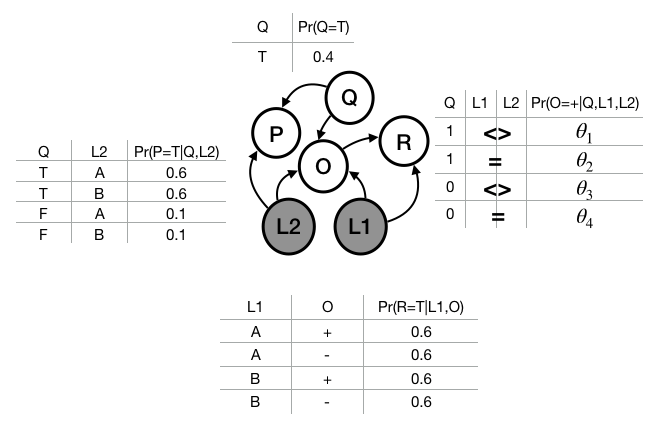
\includegraphics[width=\textwidth]{figs/BN.png}
  \end{minipage}\hfill
  \begin{minipage}[c]{0.45\textwidth}
    \caption{
        \small The model used for generating the datasets. There are four binary random variables, P, Q, O, and R. \textbf{P}: indicates whether or not the employee has high performance; \textbf{Q}: indicates whether or not an employee has high qualification; \textbf{O}: indicates whether or not the colleague submits the positive opinion towards the employee;  \textbf{R}: indicates whether or not the colleague has a positive opinion towards the employee;  \textbf{L1, L2}: indicates the label of the review provider and review receiver (observed).
    } \label{fig:BN}
  \end{minipage}
\end{figure}

We show the effectiveness of FairPSL by performing an empirical evaluation. We investigate two research questions in our experiments:
\begin{description}
\item[Q1] What is the effect of the fairness threshold $\delta$ on the fairness measures $RD/RC/RR$?
\item[Q2] How is decision quality affected by imposing $\delta$-fairness constraints?
\end{description}

Note that although we present the result for specific parameters of the framework in this section, we ran extensive analysis and the results we present are representative. We implemented the MAP inference routines of PSL and FairPSL in Python, using Gurobi-8.1\footnote{\url{www.gurobi.com}} as the backend solver. The FairPSL code, code for the data generator and data is publicly available\footnote{https://github.com/gfarnadi/FairPSL}. 

\subsection{Data generation}
  
We evaluate the FairPSL inference algorithm on synthetic datasets representing the performance review scenario (introduced in Example~\ref{ex:review}). The organization hierarchy is generated synthetically. 
The organization hierarchy generator is parameterized by two numbers: the number of employees in the organization ($n$) and the number of employees managed by each manager ($k$). Each employee is randomly assigned with a label \emph{A} or \emph{B}. An examples organization hierarchy with $n$=50 and $k$=3 is shown in Figure~\ref{fig:hierachy}.

\begin{figure}
  \begin{minipage}[c]{0.3\textwidth}
    \caption{
        \small An example of an organizational hierarchy with five levels and 50 employees with k=3. Each employee either has label A (shown with grey) or B (shown with white).
    }\label{fig:hierachy} 
	\end{minipage} \hfill
    \begin{minipage}[c]{0.7\textwidth}
    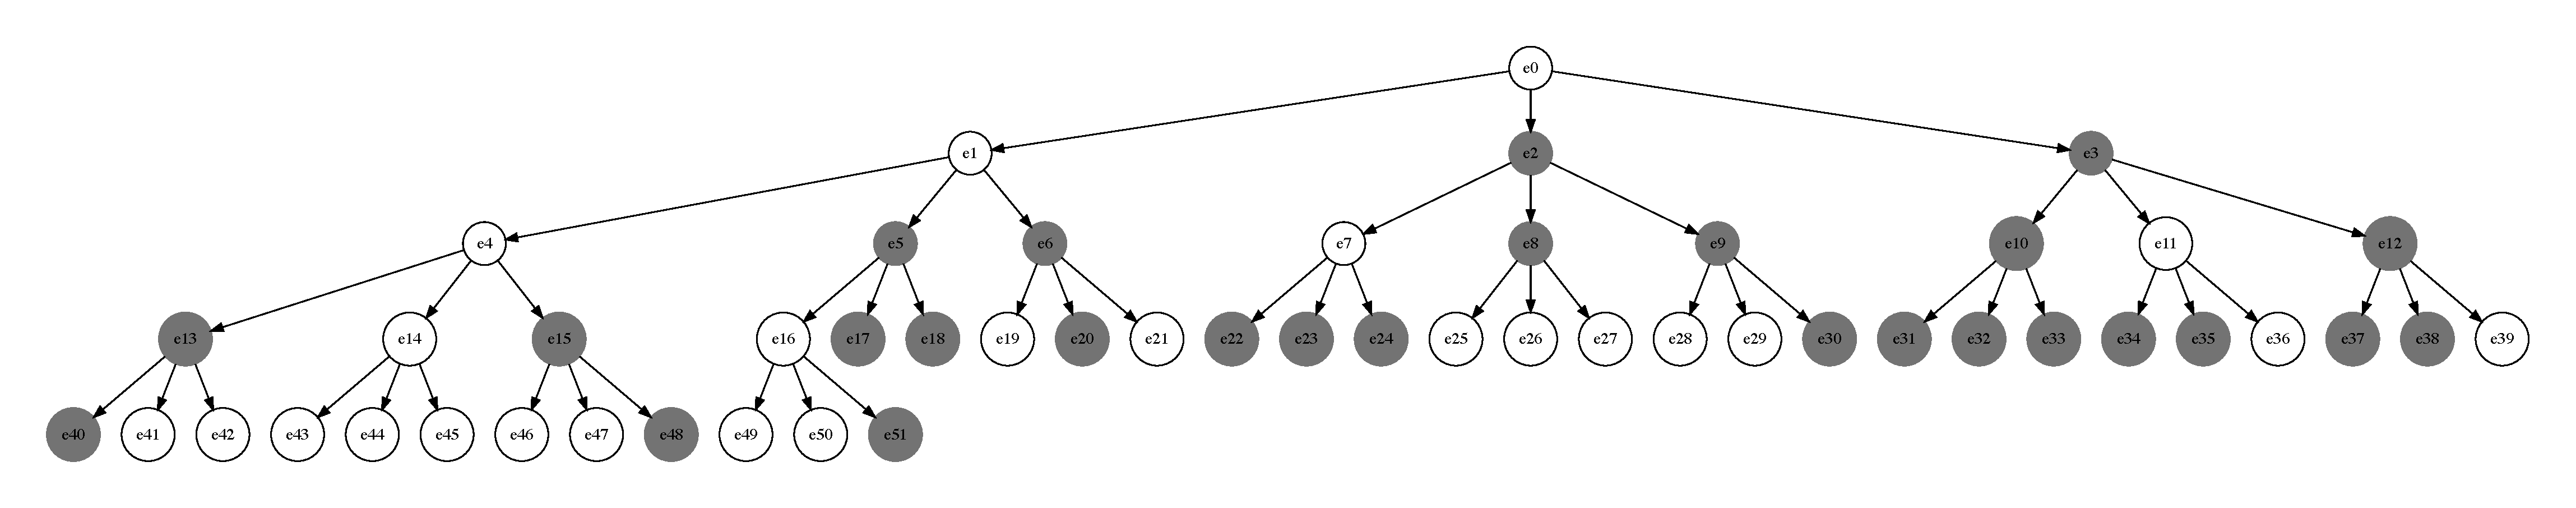
\includegraphics[width=\textwidth]{figs/Uni-hierachy.pdf}
  \end{minipage}
\end{figure}

For each employee, we use the generative model of Figure~\ref{fig:BN} to draw assignments for all the random variables. We assume that only $40\%$ of employees are qualified for promotion and regardless of their labels, employees submit only $60\%$ of their opinions. In addition, due to various personal and environmental factors, only $60\%$ of high quality employees perform well while $10\%$ of low quality employees also perform well regardless of their labels. Note that these numbers are not specific and just chosen for the framework to serve as a representative setting and a proof of concept. The conditional probability table for the opinion variable $O$ is parameterized by four values $(\theta_1, \theta_2, \theta_3, \theta_4)$ which together determine the degree of discrimination against the protected group. Since other parameters in the Bayesian network did not have a direct effect on the degree of discrimination, we fixed them to arbitrary values. 

The results presented in this section are based on an organization hierarchy  with $100$ employees where $k=5$. However, the results of the framework are not sensitive to the settings as we test the framework with various organization sizes ranging from $50$ to $500$ employees and various degree for $k$ ranging from $3$ to $10$. We generated seven datasets given the organization hierarchy using different values for the $\theta$ parameters: $(0.0,1.0,0.0,0.0)$, $(0.33,1.0,0.0,0.0)$, $(0.66,1.0,0.0,0.0)$, $(1.0,1.0,0.0,0.0)$, $(1.0,1.0,0.0,0.33)$, $(1.0,1.0,0.0,0.66)$, $(1.0,1.0,0.0,1.0)$. 
 
In the first three settings the discrimination originates from negative opinions towards qualified outgroup employees. The first setup is an extreme case where the opinion towards outgroup employees is always negative. The discrimination in the last three settings originates from positive opinions towards unqualified ingroup employees. The last setup is an extreme case where the opinion towards ingroup employees is always positive. The fourth setup represent unbiased opinions where employees are treated similarly based on their qualification. 

\paragraph{MAP Inference} We use the model presented in Table~\ref{tab:pslmodel} for MAP inference in PSL and FairPSL (recall that in FairPSL, the $\delta$-fairness constraints corresponding to one of the fairness measures are also added to the model). The observed atoms are $\textit{Manager(m,e)}$, $\textit{PositiveReview(e1,e2)}$ and labels of all employees. The truth values for all other atoms are obtained via MAP inference. We use the truth values obtained for the decision atoms $\textit{ToPromote(e)}$ to compute the fairness measures. We defined the discriminative pattern, and the protected and unprotected groups of this problem in Section~\ref{sec:formulation}.


\subsection{Evaluation results}

\begin{figure}
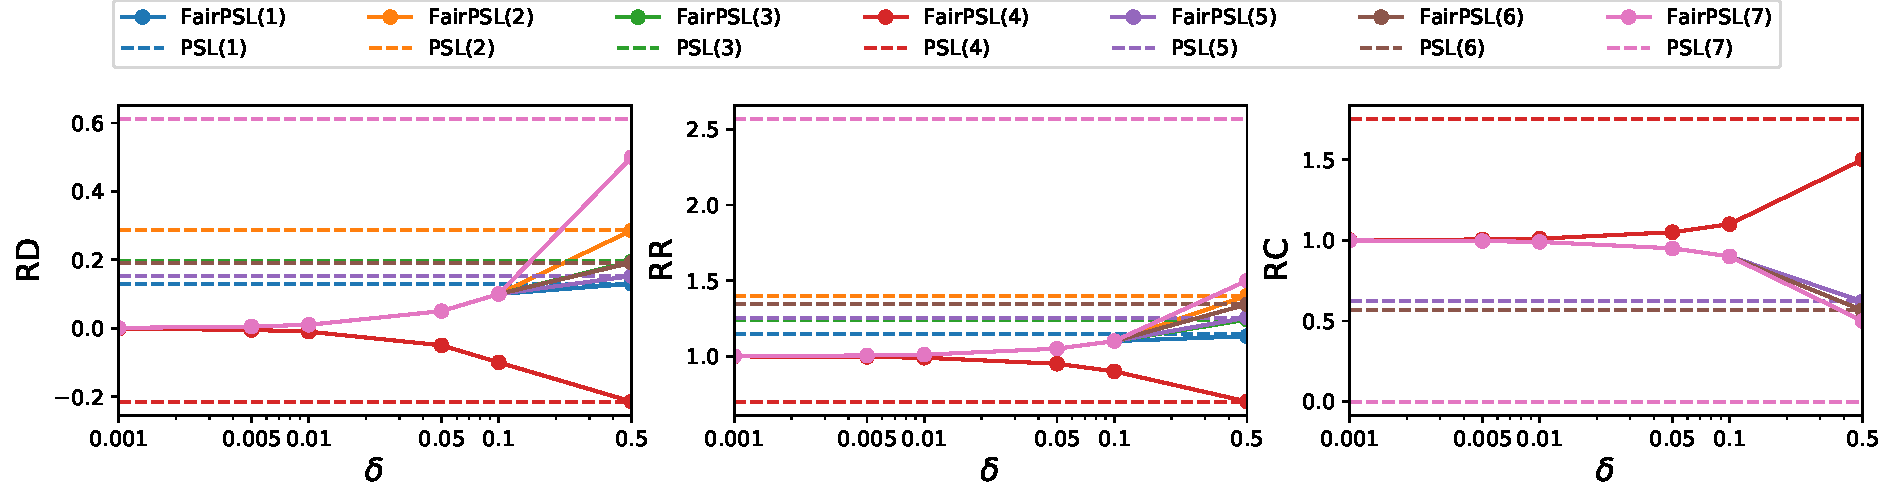
\includegraphics[width=1\linewidth]{figs/results_vis_uni_params.pdf}
\caption{\small Fairness score of predictions obtained by MAP inference of PSL and FairPSL, according to the fairness measures \emph{RD}, \emph{RR}, and \emph{RC}. The labels of datasets are mentioned with parenthesis next to the inference method. The FairPSL values of each measure are obtained by adding the $\delta$-fairness constraint of that measure.\label{fig:results}
}  
\end{figure}

To answer \textbf{Q1}, we run the MAP inference algorithm of PSL and FairPSL on seven synthetic datasets. 
We run the MAP inference of FairPSL multiple times on each dataset: For each of the three fairness measures, we add the corresponding $\delta$-fairness constraint with five thresholds $\{0.001, 0.005, 0.01, 0.05, 0.1, 0.5\}$.

Figure~\ref{fig:results} shows the fairness score of predictions in terms of the three fairness measures. As expected, tighter $\delta$-fairness constraints lead to better scores. Note that the best possible score according to RD is 0, as it computes a difference. Since RR and RC compute ratios, the best possible score according to these measures is 1. In our experiments, with any of these measures, taking $\delta = 0.001$ pushes the score of predictions to its limit.  

The $\delta$-fairness constraints modify the optimization problem of MAP inference by reducing the feasible region to solutions that conform with fairness guarantees. Research question \textbf{Q2} is concerned with the effect of this reduction on the accuracy of predictions. Note that decision quality is the same as the accuracy of predictions. To answer this question, we compare the inferred values for the decision atoms \textit{ToPromote(e)} against their actual values. These values are extracted from the known values of \textit{IsQualified(e)} according to rules 11 and 12 in Table~\ref{tab:pslmodel}. Figure~\ref{fig:accuracy} shows the area under the curve of the receiver operating characteristic~(AUC) of predicting the decision variable in three groups, namely the protected group, the unprotected group (i.e., promotion of the employees who have in-group managers), and all employees. By doing so, we make sure that our fairness constraints do not propagate bias towards either of the populations. Since the results of FairPSL with $\delta$-fairness constraints RR and RC are very similar to the results of RD, we only report the latter here.


\begin{figure}
    \centering
    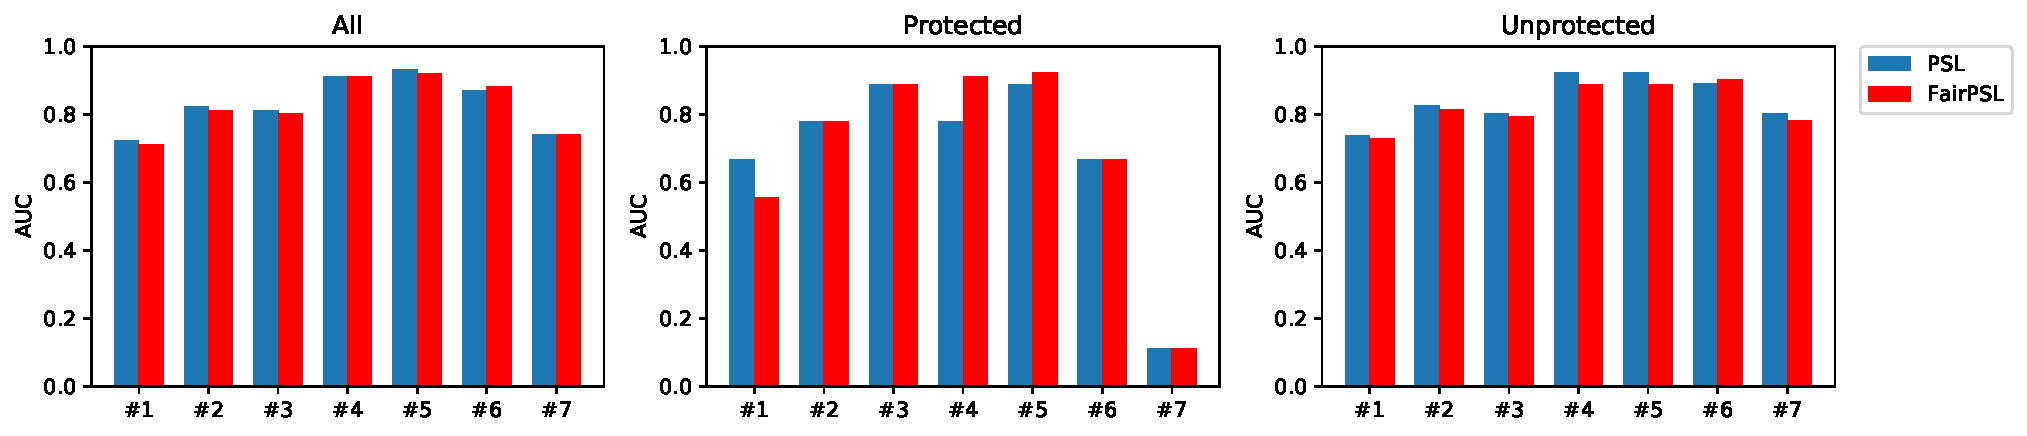
\includegraphics[width=\textwidth]{figs/roc.pdf}
    \caption{\small AUC score of predictions for truth values of unknown atoms \textit{ToPromote(e)} using MAP inference of PSL and FairPSL with $\delta$-fairness constraints $RD$ with $\delta=0.001$.}
    \label{fig:accuracy}
\end{figure}

According to Figure~\ref{fig:accuracy}, the results of both PSL and FairPSL in all seven datasets are close to each other. Note that although fairness may impose a cost in terms of overall accuracy, FairPSL often improves the accuracy of the protected class. Sometimes the overall predictions of FairPSL are even slightly better than PSL (e.g., dataset 6 and 7). As expected, the accuracy of the fourth setting where the opinions are unbiased are similar in both PSL and FairPSL. We observe that prediction of MAP inference for both FairPSL and PSL are similar, thus, in these settings at least, FairPSL guarantees fairness without hurting accuracy. Further investigation is required on the effect of the various ranges of discrimination (i.e., $\theta_1$, $\theta_2$, $\theta_3$, $\theta_4$) on the prediction results of FairPSL.



We also generate various types of organizations in which labels are not uniformly distributed, e.g., one population only occurs at the bottom levels of an organization. While we did not observe any differences in the behavior of our method with respect to accuracy and fairness measure, we found that the degree of discrimination is higher in such organizations. Further investigations on the structure of an organization on discrimination is an interesting direction for future research. 

\section{Conclusion and Future Directions}
\label{sec:conclusion}
Many applications of AI and machine learning affect peoples' lives in important ways. While there is a growing body of work on fairness in AI and ML, it assumes an individualistic notion of fairness.   In this paper, we have proposed a general framework for relational fairness which includes both a rich language for defining discrimination patterns and an efficient algorithm for performing inference subject to fairness constraints. We show our approach enforces fairness guarantees while preserving the accuracy of the predictions. 

There are many avenues for expanding on this work. For example, here we assumed that the discriminative pattern is given, however an automatic mechanism to extract discriminatory situations hidden in a large amount of decision records is an important and required task. Discrimination discovery has been studied for attribute-based fairness~\cite{pedreschi2013discovery}. An interesting next step is discrimination pattern discovery in relational data.

\section*{Acknowledgements}
This work is supported by the National Science Foundation under Grant Numbers CCF-1740850 and IIS-1703331. Golnoosh Farnadi and Behrouz Babaki are  supported by postdoctoral scholarships from IVADO through the Canada First Research Excellence Fund (CFREF) grant.

\begin{thebibliography}{10}
\itemsep=1pt 
\begin{small}

\bibitem{EUlaw}
European union legislation. (a) racial equality directive, 2000; (b) employment
  equality directive, 2000; (c) gender employment directive, 2006; (d) equal
  treatment directive (proposal), 2008.

\bibitem{UKlaw}
{UK} legislation. (a) sex discrimination act, 1975, (b) race relation act,
  1976.

\bibitem{USlaw}
United nations legislation. (a) universal declaration of human rights, 1948,
  (c) convention on the elimination of all forms of racial discrimination,
  1966, (d) convention on the elimination of all forms of discrimination
  against women, 1979.

\bibitem{alshukaili:iswc16}
Duhai Alshukaili, Alvaro A.~A. Fernandes, and Norman~W. Paton.
\newblock Structuring linked data search results using probabilistic soft
  logic.
\newblock In {\em International Semantic Web Conference {(1)}}, volume 9981 of
  {\em Lecture Notes in Computer Science}, pages 3--19, 2016.

\bibitem{bach:jmlr17}
Stephen~H. Bach, Matthias Broecheler, Bert Huang, and Lise Getoor.
\newblock Hinge-loss markov random fields and probabilistic soft logic.
\newblock {\em Journal of Machine Learning Research}, 18:109:1--109:67, 2017.

\bibitem{barocas2016big2}
Solon Barocas and Andrew~D Selbst.
\newblock Big data's disparate impact.
\newblock {\em California Law Review}, 104:671, 2016.

\bibitem{boyd2014networked}
Danah Boyd, Karen Levy, and Alice Marwick.
\newblock The networked nature of algorithmic discrimination.
\newblock In {\em Data and discrimination: Collected essays}, pages 53--57.
  2014.

\bibitem{brewer1979group}
Marilynn~B Brewer.
\newblock In-group bias in the minimal intergroup situation: A
  cognitive-motivational analysis.
\newblock {\em Psychological bulletin}, 86(2):307, 1979.

\bibitem{brewer2007social}
Marilynn~B Brewer.
\newblock The social psychology of intergroup relations: Social categorization,
  ingroup bias, and outgroup prejudice.
\newblock {\em Social Psychology: Handbook of Basic Principles}, 2007.

\bibitem{chouldechova2017fair2}
Alexandra Chouldechova.
\newblock Fair prediction with disparate impact: {A} study of bias in
  recidivism prediction instruments.
\newblock {\em CoRR}, abs/1703.00056, 2017.

\bibitem{dwork2012fairness3}
Cynthia Dwork, Moritz Hardt, Toniann Pitassi, Omer Reingold, and Richard~S.
  Zemel.
\newblock Fairness through awareness.
\newblock In {\em {ITCS}}, pages 214--226. {ACM}, 2012.

\bibitem{ebrahimi:emnlp16}
Javid Ebrahimi, Dejing Dou, and Daniel Lowd.
\newblock Weakly supervised tweet stance classification by relational
  bootstrapping.
\newblock In {\em {EMNLP}}, pages 1012--1017. The Association for Computational
  Linguistics, 2016.

\bibitem{farnadi2018fairness}
Golnoosh Farnadi, Behrouz Babaki, and Lise Getoor.
\newblock Fairness in relational domains.
\newblock In {\em AAAI/ACM Conference on AI, Ethics, and Society (AIES)}, pages
  108--114. ACM, 2018.

\bibitem{feldman2015certifying2}
Michael Feldman, Sorelle~A. Friedler, John Moeller, Carlos Scheidegger, and
  Suresh Venkatasubramanian.
\newblock Certifying and removing disparate impact.
\newblock In {\em {KDD}}, pages 259--268. {ACM}, 2015.

\bibitem{getoor2007introduction}
Lise Getoor and Ben Taskar.
\newblock {\em {Introduction to Statistical Relational Learning}}.
\newblock MIT press Cambridge, 2007.

\bibitem{hardt2016equality3}
Moritz Hardt, Eric Price, and Nati Srebro.
\newblock Equality of opportunity in supervised learning.
\newblock In {\em {NIPS}}, pages 3315--3323, 2016.

\bibitem{kamishima2011fairness}
Toshihiro Kamishima, Shotaro Akaho, and Jun Sakuma.
\newblock Fairness-aware learning through regularization approach.
\newblock In {\em ICDMW}, pages 643--650. {IEEE} Computer Society, 2011.

\bibitem{kouki:recsys15}
Pigi Kouki, Shobeir Fakhraei, James~R. Foulds, Magdalini Eirinaki, and Lise
  Getoor.
\newblock Hyper: {A} flexible and extensible probabilistic framework for hybrid
  recommender systems.
\newblock In {\em RecSys}, pages 99--106. {ACM}, 2015.

\bibitem{counterfactualfairness}
Matt~J. Kusner, Joshua~R. Loftus, Chris Russell, and Ricardo Silva.
\newblock Counterfactual fairness.
\newblock In {\em {NIPS}}, pages 4069--4079, 2017.

\bibitem{Pedreschi:2012}
Dino Pedreschi, Salvatore Ruggieri, and Franco Turini.
\newblock A study of top-k measures for discrimination discovery.
\newblock In {\em {SAC}}, pages 126--131. {ACM}, 2012.

\bibitem{pedreschi2013discovery}
Dino Pedreschi, Salvatore Ruggieri, and Franco Turini.
\newblock The discovery of discrimination.
\newblock In {\em Discrimination and Privacy in the Information Society},
  volume~3 of {\em Studies in Applied Philosophy, Epistemology and Rational
  Ethics}, pages 91--108. Springer, 2013.

\bibitem{ridgeway2004unpacking}
Cecilia~L Ridgeway and Shelley~J Correll.
\newblock Unpacking the gender system: A theoretical perspective on gender
  beliefs and social relations.
\newblock {\em Gender \& society}, 18(4):510--531, 2004.

\bibitem{sridhar:bioinformatics16}
Dhanya Sridhar, Shobeir Fakhraei, and Lise Getoor.
\newblock A probabilistic approach for collective similarity-based drug-drug
  interaction prediction.
\newblock {\em Bioinformatics}, 32(20):3175--3182, 2016.

\bibitem{verma2018fairness2}
Sahil Verma and Julia Rubin.
\newblock Fairness definitions explained.
\newblock In {\em 2018 IEEE/ACM International Workshop on Software Fairness
  (FairWare)}, pages 1--7. IEEE, 2018.

\bibitem{west2014exploiting}
Robert West, Hristo~S. Paskov, Jure Leskovec, and Christopher Potts.
\newblock Exploiting social network structure for person-to-person sentiment
  analysis.
\newblock {\em {TACL}}, 2:297--310, 2014.

\bibitem{zafar2017parity}
Muhammad~Bilal Zafar, Isabel Valera, Manuel Gomez{-}Rodriguez, Krishna~P.
  Gummadi, and Adrian Weller.
\newblock From parity to preference-based notions of fairness in
  classification.
\newblock In {\em {NIPS}}, pages 228--238, 2017.

\bibitem{zemel2013learning}
Richard~S. Zemel, Yu~Wu, Kevin Swersky, Toniann Pitassi, and Cynthia Dwork.
\newblock Learning fair representations.
\newblock In {\em {ICML} {(3)}}, volume~28 of {\em {JMLR} Workshop and
  Conference Proceedings}, pages 325--333. JMLR.org, 2013.

\end{small}
\end{thebibliography}

\end{document}

\end{article}


\begin{article}
{External vs. Internal: An Essay on  Machine Learning Agents for  Autonomous Database Management Systems}
{Andrew Pavlo, Matthew Butrovich, Ananya Joshi, Lin Ma, Prashanth 
Menon, Dana Van Aken, Lisa Lee, Ruslan Salakhutdinov}
\graphicspath{{submissions/selfdriving/}}
%\documentclass[11pt,dvipdfm]{article}
\documentclass[11pt]{article}
\usepackage{deauthor,times,graphicx} %required
\usepackage{amsmath,amssymb}
\usepackage{multirow}
\usepackage{algorithm}
\usepackage{algpseudocode}
\usepackage{todonotes}
\usepackage{url}

% \graphicspath{{farnadi/}}

\newtheorem{mydef}{\textbf{Definition}}
\newtheorem{myex}{\textbf{Example}}
\newtheorem{mytheorem}{\textbf{Theorem}}


\begin{document}

\title{A Declarative Approach to Fairness in Relational Domains}
\author{Golnoosh Farnadi$^{1,2}$, Behrouz Babaki$^1$, Lise Getoor$^3$\\
$^1$Polytechnique Montr\'{e}al, $^2$ Mila, $^3$ UC Santa Cruz \\
farnadig@mila.quebec, behrouz.babaki@polymtl.ca, getoor@soe.ucsc.edu}

\maketitle

\begin{abstract}
AI and machine learning tools are being used with increasing frequency for decision making in domains that affect peoples' lives such as employment, education, policing and %loan approval
financial qualifications. These uses raise concerns about biases of algorithmic discrimination and have motivated the development of fairness-aware machine learning. However, existing fairness approaches are based solely on attributes of individuals. In many cases, discrimination is much more complex, and taking into account the social, organizational, and other connections between individuals is important. We introduce new notions of fairness that are able to capture the relational structure in a domain. We use first-order logic to provide a flexible and expressive language for specifying complex relational patterns of discrimination. Furthermore, we extend an existing statistical relational learning framework, probabilistic soft logic~(PSL), to incorporate our definition of relational fairness. We refer to this fairness-aware framework FairPSL. FairPSL makes use of the logical definitions of fairnesss but also supports a probabilistic interpretation. In particular, we show how to perform maximum a posteriori~(MAP) inference by exploiting probabilistic dependencies within the domain while avoiding violations of fairness guarantees. Preliminary empirical evaluation shows that we are able to make both accurate and fair decisions.
\end{abstract}

\section{Introduction}
\label{sec:introduction}

Over the past few years, AI and machine learning have become essential components in operations that drive the modern society, e.g., in financial, administrative, and educational spheres. \emph{Discrimination} happens when qualities of individuals which are not relevant to the decision making process influence the decision. Delegating decision making to an automated process raises questions about discriminating against individuals with certain traits based on biases in the data. This is especially important when the decisions have the potential to impact the lives of individuals, for example, the decisions on granting loans, assigning credit, and employment. 

\emph{Fairness} is defined as the absence of discrimination in a decision making process. The goal of \emph{fairness-aware} machine learning is to ensure that the decisions made by an algorithm do not discriminate against a population of individuals~\cite{feldman2015certifying2,boyd2014networked,hardt2016equality3}. Fairness has been well studied in the social sciences and legal scholarship (for an in-depth review see~\cite{barocas2016big2}), and there is emerging work on fairness-aware ML within the AI and computer science communities. For example, fairness through awareness/Lipschitz property~\cite{dwork2012fairness3}, individual fairness~\cite{zemel2013learning}, statistical parity/group fairness~\cite{kamishima2011fairness}, counterfactual fairness~\cite{counterfactualfairness}, demographic parity/disparate impact~\cite{feldman2015certifying2,chouldechova2017fair2}, preference-based fairness~\cite{zafar2017parity}, and equality of opportunity~\cite{hardt2016equality3}.

The existing work in fairness-aware machine learning is based on a definition of discrimination where a decision is influenced by an \emph{attribute} of an individual. An attribute value upon which discrimination is based (such as gender, race, or religion) is called a \emph{sensitive attribute}. The sensitive attribute defines a population of vulnerable individuals known as the \emph{protected group}. A fair decision-making process treats the protected group the same as the \emph{unprotected group}. 

However, in many social contexts, discrimination is the result of complex interactions and can not be described solely in terms of attributes of an individual. For example, consider an imaginary scenario in an organization in which younger female workers who have older male supervisors have lower chances of promotion than their male counterparts.\footnote{Of course, many other patterns may be possible: female bosses may promote female subordinates and discriminate against male workers, or male bosses may promote female employees.  Our goal is to provide a general framework which is able to describe arbitrarily complex discrimination patterns.} 
 This discrimination pattern involves two attributes of the individual (gender and age), a relationship with another individual (supervisor), and two attributes of the second individual. Addressing such complex cases poses two challenges. First, the concepts of discrimination and fairness need to be extended to capture not only attributes of individuals but also the relationships between them. Second, a process is required that ensures that fair decisions are made about individuals who are affected by such patterns. In this paper we address both of these challenges.
We use first-order logic (FOL) to extend the notion of fairness to the relational setting. FOL is an expressive representation for relational problems which is also widely used for learning in relational domains. Moreover, we extend an existing framework for statistical relational learning~\cite{getoor2007introduction} called probabilistic soft logic (PSL)\footnote{http://psl.linqs.org/}~\cite{bach:jmlr17}. PSL combines logic and probability for learning and reasoning over uncertain relational domains. One of the most common reasoning tasks in PSL is called maximum a posteriori (MAP) inference, which is performed by finding the most probable truth values for unknowns over a set of given evidence. We develop a new MAP inference algorithm which is able to maximize the a posteriori values of unknown variables \emph{subject to} fairness guarantees. An early version of this paper which this work builds upon and extends appeared in~\cite{farnadi2018fairness}.

\looseness-1
Our contributions are as follows: 1) we propose fairness-aware machine learning for the relational setting; 2) we extend PSL into a fairness-aware framework called FairPSL which can represent the logical definition of fairness; 3) we develop a new MAP inference algorithm which is able to maximize the posteriori values of unknown variables \emph{subject to} fairness guarantees; 4) we empirically evaluate our proposed framework on synthetic data. 

\section{Motivation}
\label{sec:motivation}

Discrimination in social contexts have been studied in the field of social psychology~\cite{brewer2007social,brewer1979group,ridgeway2004unpacking}. There is a large literature on various aspects of relational bias in social contexts such as \emph{in-group-out-group bias}, \emph{gender bias}, and \emph{ethnicity-based favoritism} that can result in discrimination. 
As an example, consider gender bias in the workplace that reflects stereotypically masculine criteria and male-based favoritism. Such gender bias 
typically places women in lower positions and negatively impacts their opportunities. Further, lack of women in leadership positions may affect the promotion of women and results in a glass ceiling that keeps women from rising beyond a certain level in the hierarchy. This scenario shows that considering  protected attributes such as gender is not always sufficient to detect the source of bias and avoid discrimination, one also has to consider the relational information, in this case the organization hierarchy. Note that this can be generalized to any ingroup/outgroup scenario where the sensitive attribute could be race, religion, age, marital-status, etc.

The existing work on designing fair algorithms in machine learning exclusively focuses on \emph{attribute-based fairness}, which is based on the following assumptions: First, there is an assumption that the individuals (sometimes referred to as units or entities) are independent and described by simple attribute vectors. Second, the group for which one wishes to ensure fairness (known as the \emph{protected group}) is defined on the basis of some attribute values. Finally, there is a decision that is associated with each individual, and the goal is to ensure that members of the protected group are subject to a fair decision (we discuss different fairness measures in Section~\ref{sec:fairnessmeasure}).  We illustrate  attribute-based fairness in the following example. 

\begin{myex}[Loan Processing]
\label{ex:loan}
A bank bases its decisions about granting a loan on attributes of the applicant. The goal is to decide whether to grant a loan to an applicant using a predictive model. The bank needs to ensure that the obey fair lending practices and ensure that gender, race, sexual orientation of applicants has no influence on the decision. In this scenario, the protected group is the historically disadvantaged applicants.  
\end{myex}
The current fairness-aware machine learning techniques are not capable of modeling relations and hence cannot be used to make the decision making model fair. However, in many decision making scenarios, especially in social and organizational settings, the domain is relational, and the protected group itself might be best represented using a relational definition. We illustrate this setting in the following scenario:
\begin{myex}[Performance Review]
\label{ex:review}
Consider an organization where decisions about the promotion of employees is based on two criteria: 1) an objective performance measure, and 2) the opinion of their direct and indirect managers above them. The opinions are inferred from the performance reviews which are collected periodically. Not every manager can submit a review for all its subordinates, this is especially the case for top-level managers who have a large number of subordinates. Hence, the opinions of managers are collectively inferred from the opinions of their sub-ordinates. However, some employees may be biased, and judge other employees unfavorably, by favoring employees who are similar to themselves (same gender, race, religion, etc.) over employees who are dissimilar. The organization needs to ensure that promotion of employees do not have any relational bias caused by in-group-out-group favoritism.

\end{myex}
Example~\ref{ex:review} describes a prediction problem over a database that consists of relations between employees. Such prediction tasks are best handled by techniques from the relational learning domain. To ensure fair prediction in such settings, we need to extend the notion of \emph{attribute-based fairness} to \emph{relational fairness}. Throughout this paper, we use the performance review problem as a running example for relational fairness.

\section{Fairness Formalism}
\label{sec:formulation}

A representation that can describe different types of entities and different relationships between them is called relational. In this section, we use first-order logic to define relational fairness. We employ first-order logic as an expressive representation formalism which can represent objects and complex relationships between them. We start by defining an atom:

\begin{mydef}[Atom]
An atom is an expression of the form $P(a_1, a_2, \ldots, a_n)$ where each argument $a_1, a_2,$ $\ldots,$ $a_n$ is either a constant or a variable. The finite set of all possible substitutions of a variable to a constant for a particular variable $a$ is called its \textit{domain} $D_{a}$. If all variables in $P(a_1, a_2, \ldots, a_n)$ are substituted by some constant from their respective domain, then we call the resulting atom a \textit{ground atom}. 
\end{mydef}

\begin{myex}
In our loan processing problem (Example~\ref{ex:loan}), we can represent applicants' attributes by atoms. For instance, atom $Female(v)$ indicates whether or not applicant $v$ is female. Similarly, we can represent relations with atoms. In the performance review problem in Example~\ref{ex:review} the atom $Manager(m,e)$ indicates whether or not employee $m$ is a direct or indirect manager of employee $e$.
\end{myex}

The relational setting provides the flexibility to express complex definitions with formulae.

\begin{mydef}[Formula] 
A formula is defined by induction: every atom is a formula. If $\alpha$ and $\beta$ are formulae, then $\alpha \vee \beta$, $\alpha \wedge \beta$, $\neg \alpha$, $\alpha \rightarrow \beta$ are formulae. If $x$ is a variable and $\alpha$ is a formula, then the quantified expressions of the form $\exists x$ $\alpha$ and $\forall x$ $\alpha$ are formulae.    
\end{mydef}

To characterize groups of individuals based on a formula, we define the notion of \emph{population}.

\begin{mydef}[Population]
We denote formula $F$ which has only one free variable $v$ (i.e., other variables in $F$ are quantified) by $F[v]$. The population defined by $F[v]$ is the set of substitutions of $v$ for which $F[v]$ holds.   
\end{mydef}


\begin{myex}
\label{ex:disformula}
Consider the formula $F[v] := \forall u, \, \textit{Manager}(u,v) \rightarrow \neg \textit{SameGroup}(u, v)$. The population specified by this formula is the set of individuals all of whose managers belong to a group different from theirs. 
\end{myex}

The truth value of a formula is derived from the truth value of atoms that it comprises, according to the rules of logic. Each possible assignment of truth values to ground atoms is called an \emph{interpretation}. 


\begin{mydef}[Interpretation]
An interpretation $I$ is a mapping that associates a truth value $I(P)$ to each ground atom $P$. For Boolean truth values, $I$ associates true to 1 and false to 0 truth values. For soft logic (see Definition~\ref{def:softlogic}) $I$ maps each ground atom $P$ to a truth value in interval $[0, 1]$.
\end{mydef}

In attribute-based fairness, it is assumed that there is a certain attribute of individuals, i.e, the sensitive attribute,  that we do not want to affect a decision. Gender, race, religion and marital status are examples of sensitive attributes. Discrimination has been defined in social science studies as a treatment in favor or against a group of individuals given their sensitive attribute. This group of individuals is the protected group. 

In a relational setting, both the sensitive attributes of an individual and their participation in various relations may have an undesired effect on the final decision. We characterize the protected group in a relational setting by means of a population. In practice, we are often interested in maintaining fairness for a specific population such as applicants, students, employees, etc. This population is then partitioned into the protected and unprotected groups. We define a \emph{discriminative pattern} which is a pair of formulae to capture these groups: 1) $F_1[v]$: to specify the difference between the protected and unprotected groups and 2) $F_2[v]$: to specify the population over which we want to maintain fairness. 

\begin{mydef}[Discriminative pattern]
A discriminative pattern is a pair $\textit{DP}[v]:=(F_1[v], F_2[v])$ , where $F_1[v]$ and $F_2[v]$ are formulae.
\end{mydef}

\begin{myex}
\label{ex:pattern}
The two formulae in the discrimination pattern $\textit{DP}[v]:= \big((\forall u, \,  \textit{Manager}(u,v) \rightarrow  \neg \textit{SameGroup}(u, v)),$ $\textit{Employee}(v)\big)$ specify two populations, namely all employees and those employees who belong to a group different from their managers.
\end{myex}

Given the definition of the discriminative pattern, we have a rich language to define the scope of the protected and unprotected groups in a relational setting.

\begin{mydef}[Protected group] Given an interpretation $I$, the protected group is a population of the form:
{$$PG :=\{ v : F_1[v] \wedge F_2[v]\}$$}
which is defined as the set of all instances hold for variable $v$ for which $F_1[v] \wedge F_2[v]$ is true under interpretation $I$, that is, $I(F_1[v] \wedge F_2[v]) = 1$. 
Similarly, the \emph{unprotected group} is a population of the form: 
{$$UG := \{ v : \neg F_1[v] \wedge  F_2[v]\}$$}
which is defined as the set of all instances hold for variable $v$ 
for which $I(\neg F_1[v] \wedge F_2[v]) = 1$. 
\end{mydef}

\begin{myex}
The protected group of the discrimination pattern specified in Example~\ref{ex:pattern} is {$PG := \big\{ v : \big(\forall u, \,$ $ \textit{Manager}(u, v) \rightarrow \neg \textit{SameGroup}(u, v)\big) \wedge \textit{Employee}(v) \big\}$} and the unprotected group is {$UG :=  \big\{ v:  \big(\exists u, \, \textit{Manager}(u,v) \wedge \textit{SameGroup}(u, v)\big) \wedge \textit{Employee}(v) \big\}$}. This means our protected group is the set of employees belonging to a group different from their managers,
and our unprotected group consists of other employees. 
\end{myex}

Discrimination is defined in terms of a treatment or decision that distinguishes between the protected and unprotected groups. Here we define the \emph{decision} atom.
\begin{mydef}[Decision atom] A decision atom $d(v)$ is an atom containing exactly one variable $v$ that specifies a decision affecting the protected group which is defined either by law or end-user.
\end{mydef}
\begin{myex}
The decision atom ${\textit ToPromote}(v)$ indicates whether or not $v$ receives a promotion.
\end{myex}

Note that the fairness formulation in this section is designed for the relational setting, however relational fairness subsumes the attribute-based fairness such that: a sensitive attribute is defined by an atom with one argument and $F_2[v]$ in discrimination pattern is $\textit{Applicant}(v)$. For example, discrimination pattern of our loan processing problem in Example~\ref{ex:loan} is of the form $\textit{DP} := ( \textit{Female}(v), \textit{Applicant}(v))$ that denotes female applicants as the protected group (i.e., $PG :=  \{ v: \textit{Female}(v) \}$) and male applicants as the unprotected group (i.e., $UG := \{ v: \neg \textit{Female}(v)\}$).


\section{Fairness Measures}
\label{sec:fairnessmeasure}

Over the past few years, many fairness measures have been introduced~\cite{verma2018fairness2}. An important class of these measures are \emph{group fairness} measures which quantify the inequality between different subgroups. Some of the most popular measures in this class include \emph{equal opportunity}, \emph{equalized odds}, and \emph{demographic parity}~\cite{hardt2016equality3}. In this paper we restrict our focus to the latter. In an attribute-value setting, demographic parity means that the decision should be independent of the protected attributes. Assume that binary variables $A$ and $C$ denote the decision and protected attributes, and the preferred value of $A$ is one. Demographic parity requires that:

\begin{equation*}
    P(A=1 | C=0) = P(A=1 | C=1)
\end{equation*}

We will now generalize this measure to the relational setting using the notations defined in Section~\ref{sec:formulation}. Let $a$ and $c$ denote the counts of denial (i.e., negative decisions) for protected and unprotected groups, and $n_{1}$ and $n_{2}$ denote their sizes, respectively. Given the decision atom $d(v)$, discriminative pattern $\textit{DP}(F_1[v], F_2[v])$, and interpretation $I$, these counts are computed by the following equations: 
{
\begin{flalign}
    & a \equiv \sum_{v \in D_v} I\big( \neg d(v) \wedge  F_1[v] \wedge F_2[v]) \label{eq:a}\\
    & c \equiv \sum_{v \in D_v} I\big( \neg d(v) \wedge  \neg F_1[v] \wedge  F_2[v]) \label{eq:c}\\
    & n_{1} \equiv \sum_{v \in D_v} I\big(F_1[v] \wedge F_2[v]) \label{eq:n1}\\
    & n_{2} \equiv \sum_{v \in D_v} I\big(\neg F_1[v] \wedge  F_2[v]) \label{eq:n2}
\end{flalign}}
The proportions of denying for protected and unprotected groups are $p_1 = \frac{a}{n_1}$ and $p_2 = \frac{c}{n_2}$, respectively. There are a number of data-driven measures~\cite{Pedreschi:2012} which quantify demographic disparity and can be defined in terms of $p_1$ and $p_2$:
\begin{itemize}
    \item \textbf{Risk difference}: $RD = p_1 - p_2$, also known as absolute risk reduction. 
    \item \textbf{Risk Ratio}: $RR = \frac{p_1}{p_2}$, also known as relative risk. 
    \item \textbf{Relative Chance}: $RC = \frac{1 - p_1}{1 - p_2}$ also, known as selection rate.
\end{itemize}
These measures have been used in the legal systems of European Union, UK, and US~\cite{EUlaw,UKlaw,USlaw}. Notice that RR is the ratio of the proportion of benefit denial between the protected and unprotected groups, while RC is the ratio of the proportion of benefit granted. Finally, we introduce the notion of $\delta$-fairness.

\begin{mydef}[$\delta$-fairness]
If a fairness measure for a decision making process falls within some $\delta$-window, then the process is \emph{$\delta\text{-fair}$}. Given $0 \leq \delta \leq 1$, the  $\delta$-windows for measures RD/RR/RC are defined as:
{\begin{flalign*}
	     - \delta \leq &RD \leq \delta \\
	     1- \delta \leq &RR \leq 1+ \delta\\
	     1- \delta \leq &RC \leq 1+ \delta
	\end{flalign*}}
\end{mydef}

To overcome the limitations of attribute-based fairness, we introduce a new statistical relational learning~(SRL) framework~\cite{getoor2007introduction} suitable for modelling fairness in relational domain. In the next section, we review probabilistic soft logic~(PSL). We then extend PSL with the definition of relational fairness introduced above in Section~\ref{sec:fairMAP}. Our fairness-aware framework, ``FairPSL'', is the first SRL framework that performs fair inference. 

\section{Background: Probabilistic Soft Logic}
\label{sec:psl}

In this section, we review the syntax and semantics of PSL, and in the next section we extend MAP inference in PSL with fairness constraints to define MAP inference in FairPSL.

PSL is a probabilistic programming language for defining hinge-loss Markov random fields~\cite{bach:jmlr17}. Unlike other SRL frameworks whose atoms are Boolean, atoms in PSL can take continuous values in the interval $[0,1]$. PSL is an expressive modeling language that can incorporate domain knowledge with first-order logical rules and has been used successfully in various domains, including bioinformatics~\cite{sridhar:bioinformatics16}, recommender systems~\cite{kouki:recsys15}, natural language processing~\cite{ebrahimi:emnlp16}, information retrieval~\cite{alshukaili:iswc16}, and social network analysis~\cite{west2014exploiting}, among many others. 
 
A PSL model is defined by a set of first-order logical rules called \emph{PSL rules}.

\begin{mydef} [PSL rule] a PSL rule $r$ is an expression of the form:
{\begin{equation}
\lambda_{r}: T_1 \land T_2 \land \ldots \land T_w \rightarrow H_1 \vee H_2 \vee \ldots \vee H_l
\end{equation}}

where { $T_1, T_2, \ldots, T_w, H_1, H_2, \ldots, H_l$} are atoms or negated atoms and { $\lambda_{r} \in \mathbb{R}^{+} \cup \infty$} is the weight of the rule $r$.  We call { $T_1 \land T_2 \land \ldots \land T_w$} the body of $r$ ($r_{body}$), and { $H_1 \vee H_2 \vee \ldots \vee H_l$} the head of $r$ ($r_{head}$).
\end{mydef}


Since atoms in PSL take on continuous values in the unit interval $[0,1]$, next we define soft logic to calculate the value of the PSL rules under an interpretation $I$.

\begin{mydef}[Soft logic]
\label{def:softlogic}
The ({$\tilde{\wedge}$}) and ({$\tilde{\vee}$}) and negation ({$\tilde{\neg}$}) are defined as follows. For {$m, n \in [0,1]$} we have: {$m \tilde{\wedge} n = \max(m+n -1, 0)$}, {$m \tilde{\vee} n = \min(m+n , 1)$} and {$\tilde{\neg} m = 1 - m$}. The $\, \tilde{} \,$ indicates the relaxation over Boolean values.
\end{mydef}

The probability of truth value assignments in PSL is determined by the rules' \emph{distance to satisfaction}.

\begin{mydef}[The distance to satisfaction]
The distance to satisfaction $d_{r}(I)$ of a rule $r$ under an interpretation $I$ is defined as:
{
\begin{equation}
d_{r}(I) = \max\{0, I(r_{body})-I(r_{head})\}
\end{equation}}
\end{mydef}

By using Definition~\ref{def:softlogic}, one can show that the closer the interpretation of a grounded rule $r$ is to 1, the smaller its distance to satisfaction. A PSL model induces a distribution over interpretations $I$. Let $R$ be the set of all grounded rules, then the probability density function is:
{
\begin{equation}
f(I) ={\frac{1}{Z}} \exp[-\sum_{r\in R} \lambda_{r}(d_{r}(I))^p]
\label{eq:potential}
\end{equation}
}
\noindent where { $\lambda_{r}$} is the weight of rule $r$, {
$Z = \int_{I} \exp[ -\sum_{r\in R} \lambda_{r}(d_{r}(I))^p]$
} is a normalization constant, and { $p \in \{1,2\}$} provides a choice of two different loss functions, $p=1$ (i.e., linear), and $p=2$ (i.e, quadratic). These probabilistic models are instances of hinge-loss Markov random fields~(HL-MRF)~\cite{bach:jmlr17}. The goal of maximum a posteriori (MAP) inference is to find the most probable truth assignments $I_{\textit{MPE}}$ of unknown ground atoms given the evidence which is defined by the interpretation $I$. Let $X$ be all the evidence, i.e., $X$ is the set of ground atoms such that $\forall x \in X, I(x)$ is known, and let $Y$ be the set of ground atoms such that $\forall y \in Y, I(y)$ is unknown. Then we have
{
\begin{equation}
I_{\textit{MAP}}(Y) = \textit{arg}\max_{I(Y)} P(I(Y)|I(X))
\end{equation}}
Maximizing the density function in Equation~\ref{eq:potential} is equivalent to minimizing the weighted sum of the distances to satisfaction of all rules in PSL. 

\begin{table*}[t]
    \centering
    \begin{tabular}{|lll|}
    \hline
    &&\\
    $R1$ & $\lambda_1$ &: $\textit{IsQualified}(e) \rightarrow \textit{HighPerformance}(e)$ \\
    $R2$ & $\lambda_1$ &: $\neg \textit{IsQualified}(e) \rightarrow \neg \textit{HighPerformance}(e)$ \\
    $R3$ & $\infty$ &: $\textit{PositiveReview}(e1, e2) \rightarrow \textit{PositiveOpinion}(e1, e2)$ \\
    $R4$ & $\infty$ &: $\neg \textit{PositiveReview}(e1, e2) \rightarrow \neg \textit{PositiveOpinion}(e1, e2)$ \\
    $R5$ & $\lambda_1$ &: $\textit{PositiveOpinion}(e1, e2) \wedge \textit{Manager}(m, e1) \rightarrow \textit{PositiveOpinion}(m, e2)$ \\
    $R6$ & $\lambda_1$ &: $\neg \textit{PositiveOpinion}(e1, e2) \wedge \textit{Manager}(m, e1) \rightarrow \neg \textit{PositiveOpinion}(m, e2)$ \\
    $R7$ & $\lambda_1$ &: $\textit{PositiveOpinion}(m, e) \wedge \textit{Manager}(m, e) \rightarrow \textit{IsQualified}(e)$ \\
    $R8$ & $\lambda_1$ &: $\neg \textit{PositiveOpinion}(m, e) \wedge \textit{Manager}(m, e) \rightarrow \neg \textit{IsQualified}(e)$ \\
    $R9$ &  $\lambda_1$ &: $\neg \textit{ToPromote}(e)$\\
    $R10$ & $\infty$ &: $\textit{IsQualified}(e) \rightarrow \textit{ToPromote}(e)$ \\
    $R11$ & $\infty$ &: $\neg \textit{IsQualified}(e) \rightarrow \neg \textit{ToPromote}(e)$ \\
    &&\\
    \hline
    \end{tabular}
    \caption{\small A simplified PSL model for the \emph{Performance Reviewing} problem}
    \label{tab:pslmodel}
\end{table*}

\begin{myex}
\label{ex:pslmodel}
The simplified PSL model for the performance reviewing problem in Example\ref{ex:review} is given in Table~\ref{tab:pslmodel}. The goal of MAP inference for this problem is to infer employees to promote. We simplified the model by assigning the same weight to all soft rules (i.e., $\lambda_i= 1$ where $i=\{1,2,5,6,7,8,9\}$). Below we explain the meaning of each rule in the model.

Rule $R1$ indicates that qualified employees have high performance and similarly rule $R2$ expresses that a negative qualification of employees is derived from their low performance. Rules $R5$ and $R6$ presents the propagation of opinion from bottom to top of the organizational hierarchy, i.e., managers have similar opinions towards employees given the opinions of their sub-ordinate managers. And rules $R7$ and $R8$ indicate that the positive/negative opinion of direct/indirect managers derive from the qualification of an employee. Rule $R9$ indicates the prior that not all employees get promoted. We also have four hard constraints (i.e., rules $R3$, $R4$, $R10$ and $R11$) where the weight of the rules are $\infty$. Rules $R3$ and $R4$ indicate that submitted positive/negative reviews should reflect positive/negative opinions. And two rules $R10$ and $R11$ show that a highly qualified employee should get promoted. 
\end{myex}

\section{Fairness-aware PSL (FairPSL)}
\label{sec:fairMAP}

The standard MAP inference in PSL aims at finding values that maximize the conditional probability of unknowns. Once a decision is made according to these values, one can use the fairness measure to quantify the degree of discrimination. A simple way to incorporate fairness in MAP inference is to add the $\delta$-fairness constraints to the corresponding optimization problem.   

Consider risk difference, $\textit{RD}$, where $\textit{RD} \equiv \frac{\mathbf{a}}{n_1} - \frac{\mathbf{c}}{n_2}$. The $\delta$-fairness constraint $-\delta \leq \textit{RD} \leq \delta$ can be encoded as the following constraints:
{\begin{align}
    & n_2 \mathbf{a} - n_1 \mathbf{c} - n_1 n_2 \delta \leq 0 \label{eq:RD1}\\
    & n_2 \mathbf{a} - n_1 \mathbf{c} + n_1 n_2 \delta \geq 0
\end{align}}
Similarly, from $\textit{RR} \equiv \frac{\mathbf{a} / n_1}{\mathbf{c} / n_2}$ and the $\delta$-fairness constraint $1 - \delta \leq \textit{RR} \leq 1 + \delta$ we obtain:
{\begin{align}
    & n_2 \mathbf{a} - (1 + \delta) n_1 \mathbf{c} \leq 0 \\
    & n_2 \mathbf{a} - (1 - \delta) n_1 \mathbf{c} \geq 0
\end{align}}
And finally, $\textit{RC} \equiv \frac{1 - \mathbf{a} / n_1}{1 - \mathbf{c} / n_2}$ and the $\delta$-fairness constraint $1 - \delta \leq \textit{RC} \leq 1 + \delta$ gives:
{ \begin{align}
    & - n_2 \mathbf{a} + (1 + \delta) n_1 \mathbf{c} - \delta n_1 n_2 \leq 0 \\
    & - n_2 \mathbf{a} + (1 - \delta) n_1 \mathbf{c} + \delta n_1 n_2 \geq 0 \label{eq:RC2}
\end{align}}
A primary advantage of PSL over similar frameworks is that its MAP inference task reduces to a convex optimization problem which can be solved in polynomial time. To preserve this advantage, we need to ensure that the problem will remain convex after the addition of $\delta$-fairness constraints. 

\begin{mytheorem}
The following condition is sufficient for preserving the convexity of MAP inference problem after addition of $\delta$-fairness constraints: The formulae $F_1[v]$ and $F_2[v]$ do not contain an atom $y \in Y$ and all atoms in $F_1[v]$ and $F_2[v]$ have values zero or one.
\end{mytheorem}
\begin{proof}
Since $I(F_1[v])$ and $I(F_2[v])$ do not depend on $I(Y)$, the values $n_{1}$ and $n_{2}$ are constants that can be computed in advance. Let us define the sets $D_v^a = \{ v \in D_v : F_1[v] \wedge F_2[v] \, \text{is true} \}$ and $D_v^c = \{ v \in D_v : \neg F_1[v] \wedge F_2[v] \, \text{is true} \}$. Since $F_1[v]$ and $F_2[v]$ can be only zero or one, we can rewrite the equations~\ref{eq:a} and \ref{eq:c} as:
{
\begin{align*}
    & \mathbf{a} = \sum_{v \in D_v^a} I(\neg d(v)) = |D_v^a| - \sum_{v \in D_v^a} I(d(v))\\
    & \mathbf{c} = \sum_{v \in D_v^c} I(\neg d(v)) = |D_v^c| - \sum_{v \in D_v^c} I(d(v))
\end{align*}}
\noindent which indicates that $\mathbf{a}$ and $\mathbf{c}$ can be expressed as linear combinations of variables in the optimization problem. This means that constraints~\ref{eq:RD1}-\ref{eq:RC2} are linear. Hence, addition of these constraints preserves the convexity of the optimization problem. 
\end{proof}

\section{Experiments}
\label{sec:experiment}

\begin{figure}
  \begin{minipage}[c]{0.6\textwidth}
    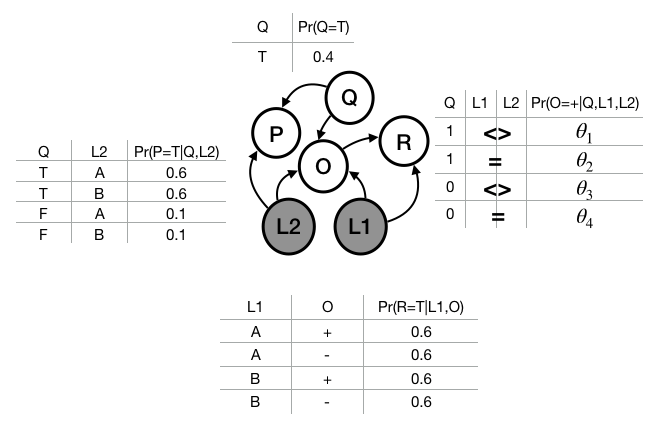
\includegraphics[width=\textwidth]{figs/BN.png}
  \end{minipage}\hfill
  \begin{minipage}[c]{0.45\textwidth}
    \caption{
        \small The model used for generating the datasets. There are four binary random variables, P, Q, O, and R. \textbf{P}: indicates whether or not the employee has high performance; \textbf{Q}: indicates whether or not an employee has high qualification; \textbf{O}: indicates whether or not the colleague submits the positive opinion towards the employee;  \textbf{R}: indicates whether or not the colleague has a positive opinion towards the employee;  \textbf{L1, L2}: indicates the label of the review provider and review receiver (observed).
    } \label{fig:BN}
  \end{minipage}
\end{figure}

We show the effectiveness of FairPSL by performing an empirical evaluation. We investigate two research questions in our experiments:
\begin{description}
\item[Q1] What is the effect of the fairness threshold $\delta$ on the fairness measures $RD/RC/RR$?
\item[Q2] How is decision quality affected by imposing $\delta$-fairness constraints?
\end{description}

Note that although we present the result for specific parameters of the framework in this section, we ran extensive analysis and the results we present are representative. We implemented the MAP inference routines of PSL and FairPSL in Python, using Gurobi-8.1\footnote{\url{www.gurobi.com}} as the backend solver. The FairPSL code, code for the data generator and data is publicly available\footnote{https://github.com/gfarnadi/FairPSL}. 

\subsection{Data generation}
  
We evaluate the FairPSL inference algorithm on synthetic datasets representing the performance review scenario (introduced in Example~\ref{ex:review}). The organization hierarchy is generated synthetically. 
The organization hierarchy generator is parameterized by two numbers: the number of employees in the organization ($n$) and the number of employees managed by each manager ($k$). Each employee is randomly assigned with a label \emph{A} or \emph{B}. An examples organization hierarchy with $n$=50 and $k$=3 is shown in Figure~\ref{fig:hierachy}.

\begin{figure}
  \begin{minipage}[c]{0.3\textwidth}
    \caption{
        \small An example of an organizational hierarchy with five levels and 50 employees with k=3. Each employee either has label A (shown with grey) or B (shown with white).
    }\label{fig:hierachy} 
	\end{minipage} \hfill
    \begin{minipage}[c]{0.7\textwidth}
    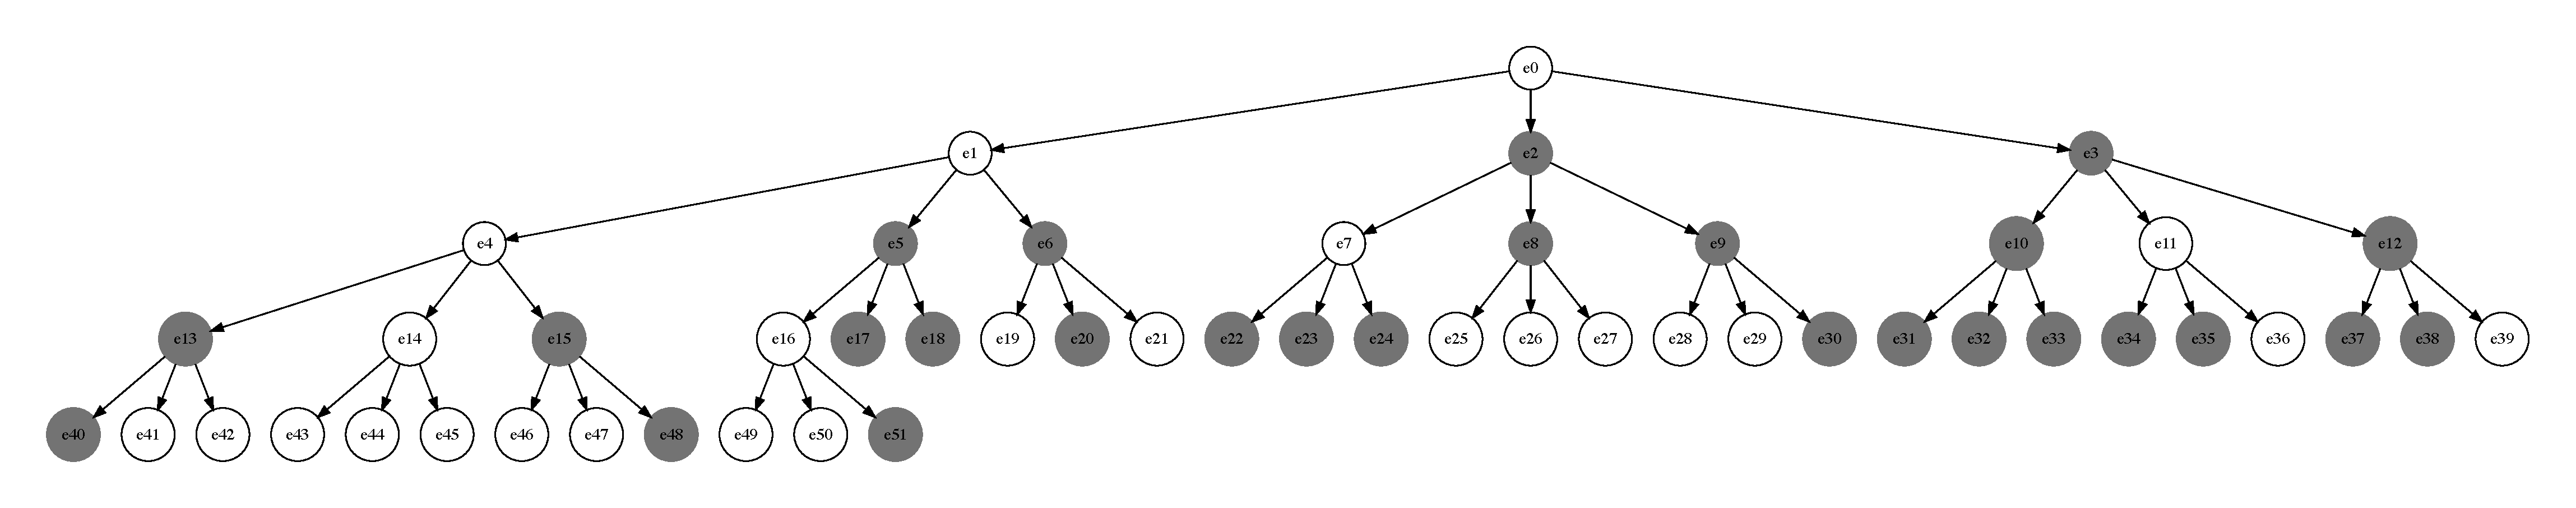
\includegraphics[width=\textwidth]{figs/Uni-hierachy.pdf}
  \end{minipage}
\end{figure}

For each employee, we use the generative model of Figure~\ref{fig:BN} to draw assignments for all the random variables. We assume that only $40\%$ of employees are qualified for promotion and regardless of their labels, employees submit only $60\%$ of their opinions. In addition, due to various personal and environmental factors, only $60\%$ of high quality employees perform well while $10\%$ of low quality employees also perform well regardless of their labels. Note that these numbers are not specific and just chosen for the framework to serve as a representative setting and a proof of concept. The conditional probability table for the opinion variable $O$ is parameterized by four values $(\theta_1, \theta_2, \theta_3, \theta_4)$ which together determine the degree of discrimination against the protected group. Since other parameters in the Bayesian network did not have a direct effect on the degree of discrimination, we fixed them to arbitrary values. 

The results presented in this section are based on an organization hierarchy  with $100$ employees where $k=5$. However, the results of the framework are not sensitive to the settings as we test the framework with various organization sizes ranging from $50$ to $500$ employees and various degree for $k$ ranging from $3$ to $10$. We generated seven datasets given the organization hierarchy using different values for the $\theta$ parameters: $(0.0,1.0,0.0,0.0)$, $(0.33,1.0,0.0,0.0)$, $(0.66,1.0,0.0,0.0)$, $(1.0,1.0,0.0,0.0)$, $(1.0,1.0,0.0,0.33)$, $(1.0,1.0,0.0,0.66)$, $(1.0,1.0,0.0,1.0)$. 
 
In the first three settings the discrimination originates from negative opinions towards qualified outgroup employees. The first setup is an extreme case where the opinion towards outgroup employees is always negative. The discrimination in the last three settings originates from positive opinions towards unqualified ingroup employees. The last setup is an extreme case where the opinion towards ingroup employees is always positive. The fourth setup represent unbiased opinions where employees are treated similarly based on their qualification. 

\paragraph{MAP Inference} We use the model presented in Table~\ref{tab:pslmodel} for MAP inference in PSL and FairPSL (recall that in FairPSL, the $\delta$-fairness constraints corresponding to one of the fairness measures are also added to the model). The observed atoms are $\textit{Manager(m,e)}$, $\textit{PositiveReview(e1,e2)}$ and labels of all employees. The truth values for all other atoms are obtained via MAP inference. We use the truth values obtained for the decision atoms $\textit{ToPromote(e)}$ to compute the fairness measures. We defined the discriminative pattern, and the protected and unprotected groups of this problem in Section~\ref{sec:formulation}.


\subsection{Evaluation results}

\begin{figure}
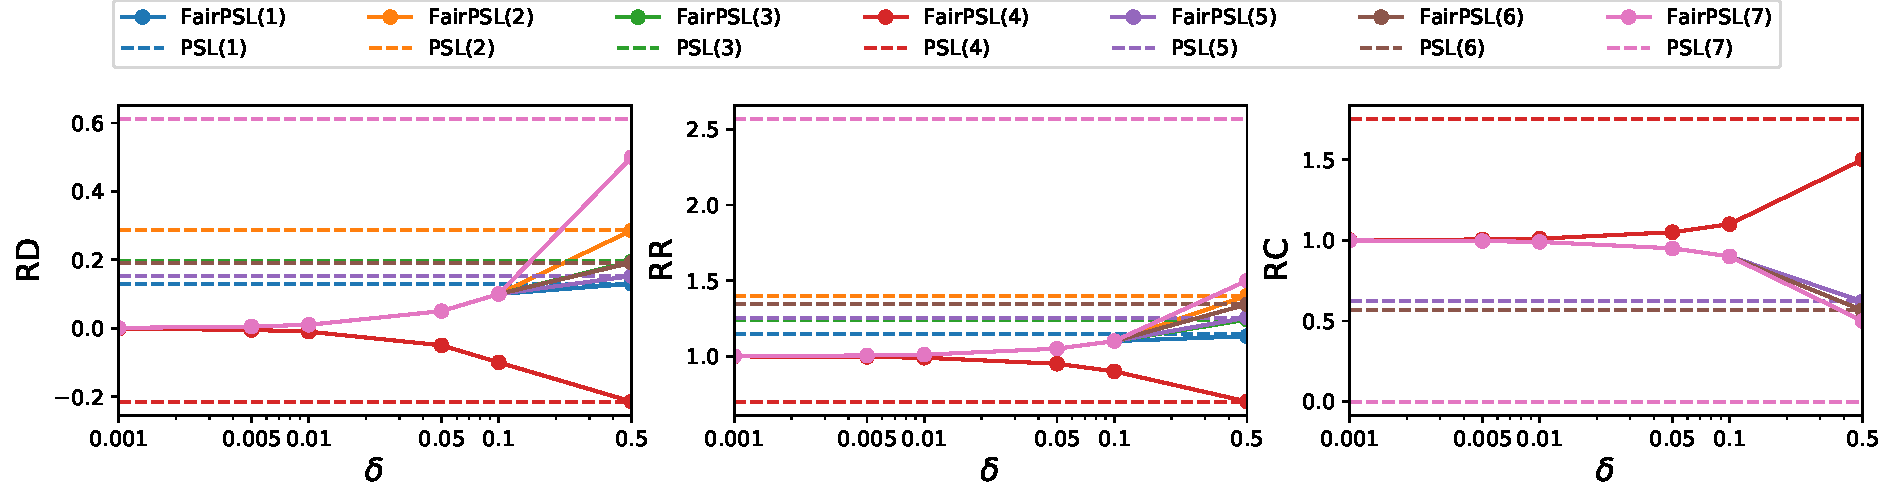
\includegraphics[width=1\linewidth]{figs/results_vis_uni_params.pdf}
\caption{\small Fairness score of predictions obtained by MAP inference of PSL and FairPSL, according to the fairness measures \emph{RD}, \emph{RR}, and \emph{RC}. The labels of datasets are mentioned with parenthesis next to the inference method. The FairPSL values of each measure are obtained by adding the $\delta$-fairness constraint of that measure.\label{fig:results}
}  
\end{figure}

To answer \textbf{Q1}, we run the MAP inference algorithm of PSL and FairPSL on seven synthetic datasets. 
We run the MAP inference of FairPSL multiple times on each dataset: For each of the three fairness measures, we add the corresponding $\delta$-fairness constraint with five thresholds $\{0.001, 0.005, 0.01, 0.05, 0.1, 0.5\}$.

Figure~\ref{fig:results} shows the fairness score of predictions in terms of the three fairness measures. As expected, tighter $\delta$-fairness constraints lead to better scores. Note that the best possible score according to RD is 0, as it computes a difference. Since RR and RC compute ratios, the best possible score according to these measures is 1. In our experiments, with any of these measures, taking $\delta = 0.001$ pushes the score of predictions to its limit.  

The $\delta$-fairness constraints modify the optimization problem of MAP inference by reducing the feasible region to solutions that conform with fairness guarantees. Research question \textbf{Q2} is concerned with the effect of this reduction on the accuracy of predictions. Note that decision quality is the same as the accuracy of predictions. To answer this question, we compare the inferred values for the decision atoms \textit{ToPromote(e)} against their actual values. These values are extracted from the known values of \textit{IsQualified(e)} according to rules 11 and 12 in Table~\ref{tab:pslmodel}. Figure~\ref{fig:accuracy} shows the area under the curve of the receiver operating characteristic~(AUC) of predicting the decision variable in three groups, namely the protected group, the unprotected group (i.e., promotion of the employees who have in-group managers), and all employees. By doing so, we make sure that our fairness constraints do not propagate bias towards either of the populations. Since the results of FairPSL with $\delta$-fairness constraints RR and RC are very similar to the results of RD, we only report the latter here.


\begin{figure}
    \centering
    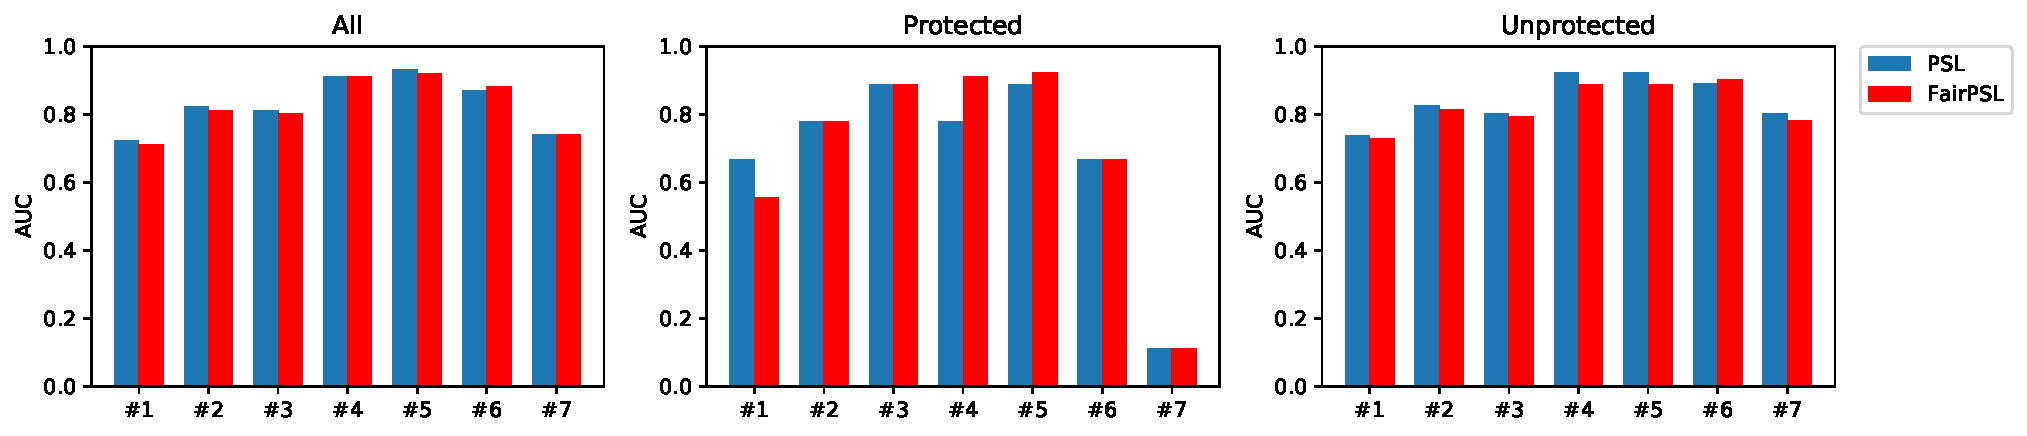
\includegraphics[width=\textwidth]{figs/roc.pdf}
    \caption{\small AUC score of predictions for truth values of unknown atoms \textit{ToPromote(e)} using MAP inference of PSL and FairPSL with $\delta$-fairness constraints $RD$ with $\delta=0.001$.}
    \label{fig:accuracy}
\end{figure}

According to Figure~\ref{fig:accuracy}, the results of both PSL and FairPSL in all seven datasets are close to each other. Note that although fairness may impose a cost in terms of overall accuracy, FairPSL often improves the accuracy of the protected class. Sometimes the overall predictions of FairPSL are even slightly better than PSL (e.g., dataset 6 and 7). As expected, the accuracy of the fourth setting where the opinions are unbiased are similar in both PSL and FairPSL. We observe that prediction of MAP inference for both FairPSL and PSL are similar, thus, in these settings at least, FairPSL guarantees fairness without hurting accuracy. Further investigation is required on the effect of the various ranges of discrimination (i.e., $\theta_1$, $\theta_2$, $\theta_3$, $\theta_4$) on the prediction results of FairPSL.



We also generate various types of organizations in which labels are not uniformly distributed, e.g., one population only occurs at the bottom levels of an organization. While we did not observe any differences in the behavior of our method with respect to accuracy and fairness measure, we found that the degree of discrimination is higher in such organizations. Further investigations on the structure of an organization on discrimination is an interesting direction for future research. 

\section{Conclusion and Future Directions}
\label{sec:conclusion}
Many applications of AI and machine learning affect peoples' lives in important ways. While there is a growing body of work on fairness in AI and ML, it assumes an individualistic notion of fairness.   In this paper, we have proposed a general framework for relational fairness which includes both a rich language for defining discrimination patterns and an efficient algorithm for performing inference subject to fairness constraints. We show our approach enforces fairness guarantees while preserving the accuracy of the predictions. 

There are many avenues for expanding on this work. For example, here we assumed that the discriminative pattern is given, however an automatic mechanism to extract discriminatory situations hidden in a large amount of decision records is an important and required task. Discrimination discovery has been studied for attribute-based fairness~\cite{pedreschi2013discovery}. An interesting next step is discrimination pattern discovery in relational data.

\section*{Acknowledgements}
This work is supported by the National Science Foundation under Grant Numbers CCF-1740850 and IIS-1703331. Golnoosh Farnadi and Behrouz Babaki are  supported by postdoctoral scholarships from IVADO through the Canada First Research Excellence Fund (CFREF) grant.

\begin{thebibliography}{10}
\itemsep=1pt 
\begin{small}

\bibitem{EUlaw}
European union legislation. (a) racial equality directive, 2000; (b) employment
  equality directive, 2000; (c) gender employment directive, 2006; (d) equal
  treatment directive (proposal), 2008.

\bibitem{UKlaw}
{UK} legislation. (a) sex discrimination act, 1975, (b) race relation act,
  1976.

\bibitem{USlaw}
United nations legislation. (a) universal declaration of human rights, 1948,
  (c) convention on the elimination of all forms of racial discrimination,
  1966, (d) convention on the elimination of all forms of discrimination
  against women, 1979.

\bibitem{alshukaili:iswc16}
Duhai Alshukaili, Alvaro A.~A. Fernandes, and Norman~W. Paton.
\newblock Structuring linked data search results using probabilistic soft
  logic.
\newblock In {\em International Semantic Web Conference {(1)}}, volume 9981 of
  {\em Lecture Notes in Computer Science}, pages 3--19, 2016.

\bibitem{bach:jmlr17}
Stephen~H. Bach, Matthias Broecheler, Bert Huang, and Lise Getoor.
\newblock Hinge-loss markov random fields and probabilistic soft logic.
\newblock {\em Journal of Machine Learning Research}, 18:109:1--109:67, 2017.

\bibitem{barocas2016big2}
Solon Barocas and Andrew~D Selbst.
\newblock Big data's disparate impact.
\newblock {\em California Law Review}, 104:671, 2016.

\bibitem{boyd2014networked}
Danah Boyd, Karen Levy, and Alice Marwick.
\newblock The networked nature of algorithmic discrimination.
\newblock In {\em Data and discrimination: Collected essays}, pages 53--57.
  2014.

\bibitem{brewer1979group}
Marilynn~B Brewer.
\newblock In-group bias in the minimal intergroup situation: A
  cognitive-motivational analysis.
\newblock {\em Psychological bulletin}, 86(2):307, 1979.

\bibitem{brewer2007social}
Marilynn~B Brewer.
\newblock The social psychology of intergroup relations: Social categorization,
  ingroup bias, and outgroup prejudice.
\newblock {\em Social Psychology: Handbook of Basic Principles}, 2007.

\bibitem{chouldechova2017fair2}
Alexandra Chouldechova.
\newblock Fair prediction with disparate impact: {A} study of bias in
  recidivism prediction instruments.
\newblock {\em CoRR}, abs/1703.00056, 2017.

\bibitem{dwork2012fairness3}
Cynthia Dwork, Moritz Hardt, Toniann Pitassi, Omer Reingold, and Richard~S.
  Zemel.
\newblock Fairness through awareness.
\newblock In {\em {ITCS}}, pages 214--226. {ACM}, 2012.

\bibitem{ebrahimi:emnlp16}
Javid Ebrahimi, Dejing Dou, and Daniel Lowd.
\newblock Weakly supervised tweet stance classification by relational
  bootstrapping.
\newblock In {\em {EMNLP}}, pages 1012--1017. The Association for Computational
  Linguistics, 2016.

\bibitem{farnadi2018fairness}
Golnoosh Farnadi, Behrouz Babaki, and Lise Getoor.
\newblock Fairness in relational domains.
\newblock In {\em AAAI/ACM Conference on AI, Ethics, and Society (AIES)}, pages
  108--114. ACM, 2018.

\bibitem{feldman2015certifying2}
Michael Feldman, Sorelle~A. Friedler, John Moeller, Carlos Scheidegger, and
  Suresh Venkatasubramanian.
\newblock Certifying and removing disparate impact.
\newblock In {\em {KDD}}, pages 259--268. {ACM}, 2015.

\bibitem{getoor2007introduction}
Lise Getoor and Ben Taskar.
\newblock {\em {Introduction to Statistical Relational Learning}}.
\newblock MIT press Cambridge, 2007.

\bibitem{hardt2016equality3}
Moritz Hardt, Eric Price, and Nati Srebro.
\newblock Equality of opportunity in supervised learning.
\newblock In {\em {NIPS}}, pages 3315--3323, 2016.

\bibitem{kamishima2011fairness}
Toshihiro Kamishima, Shotaro Akaho, and Jun Sakuma.
\newblock Fairness-aware learning through regularization approach.
\newblock In {\em ICDMW}, pages 643--650. {IEEE} Computer Society, 2011.

\bibitem{kouki:recsys15}
Pigi Kouki, Shobeir Fakhraei, James~R. Foulds, Magdalini Eirinaki, and Lise
  Getoor.
\newblock Hyper: {A} flexible and extensible probabilistic framework for hybrid
  recommender systems.
\newblock In {\em RecSys}, pages 99--106. {ACM}, 2015.

\bibitem{counterfactualfairness}
Matt~J. Kusner, Joshua~R. Loftus, Chris Russell, and Ricardo Silva.
\newblock Counterfactual fairness.
\newblock In {\em {NIPS}}, pages 4069--4079, 2017.

\bibitem{Pedreschi:2012}
Dino Pedreschi, Salvatore Ruggieri, and Franco Turini.
\newblock A study of top-k measures for discrimination discovery.
\newblock In {\em {SAC}}, pages 126--131. {ACM}, 2012.

\bibitem{pedreschi2013discovery}
Dino Pedreschi, Salvatore Ruggieri, and Franco Turini.
\newblock The discovery of discrimination.
\newblock In {\em Discrimination and Privacy in the Information Society},
  volume~3 of {\em Studies in Applied Philosophy, Epistemology and Rational
  Ethics}, pages 91--108. Springer, 2013.

\bibitem{ridgeway2004unpacking}
Cecilia~L Ridgeway and Shelley~J Correll.
\newblock Unpacking the gender system: A theoretical perspective on gender
  beliefs and social relations.
\newblock {\em Gender \& society}, 18(4):510--531, 2004.

\bibitem{sridhar:bioinformatics16}
Dhanya Sridhar, Shobeir Fakhraei, and Lise Getoor.
\newblock A probabilistic approach for collective similarity-based drug-drug
  interaction prediction.
\newblock {\em Bioinformatics}, 32(20):3175--3182, 2016.

\bibitem{verma2018fairness2}
Sahil Verma and Julia Rubin.
\newblock Fairness definitions explained.
\newblock In {\em 2018 IEEE/ACM International Workshop on Software Fairness
  (FairWare)}, pages 1--7. IEEE, 2018.

\bibitem{west2014exploiting}
Robert West, Hristo~S. Paskov, Jure Leskovec, and Christopher Potts.
\newblock Exploiting social network structure for person-to-person sentiment
  analysis.
\newblock {\em {TACL}}, 2:297--310, 2014.

\bibitem{zafar2017parity}
Muhammad~Bilal Zafar, Isabel Valera, Manuel Gomez{-}Rodriguez, Krishna~P.
  Gummadi, and Adrian Weller.
\newblock From parity to preference-based notions of fairness in
  classification.
\newblock In {\em {NIPS}}, pages 228--238, 2017.

\bibitem{zemel2013learning}
Richard~S. Zemel, Yu~Wu, Kevin Swersky, Toniann Pitassi, and Cynthia Dwork.
\newblock Learning fair representations.
\newblock In {\em {ICML} {(3)}}, volume~28 of {\em {JMLR} Workshop and
  Conference Proceedings}, pages 325--333. JMLR.org, 2013.

\end{small}
\end{thebibliography}

\end{document}

\end{article}



\begin{article}
{Learning Data Structure Alchemy}
{Stratos Idreos, 
Kostas Zoumpatianos, 
Subarna Chatterjee, 
Wilson Qin,
Abdul Wasay,
Brian Hentschel, 
Mike Kester,
Niv Dayan,
Demi Guo,
Minseo Kang,
Yiyou Sun
}
\graphicspath{{submissions/Learning/}}
%\documentclass[11pt,dvipdfm]{article}
\documentclass[11pt]{article}
\usepackage{deauthor,times,graphicx} %required
\usepackage{amsmath,amssymb}
\usepackage{multirow}
\usepackage{algorithm}
\usepackage{algpseudocode}
\usepackage{todonotes}
\usepackage{url}

% \graphicspath{{farnadi/}}

\newtheorem{mydef}{\textbf{Definition}}
\newtheorem{myex}{\textbf{Example}}
\newtheorem{mytheorem}{\textbf{Theorem}}


\begin{document}

\title{A Declarative Approach to Fairness in Relational Domains}
\author{Golnoosh Farnadi$^{1,2}$, Behrouz Babaki$^1$, Lise Getoor$^3$\\
$^1$Polytechnique Montr\'{e}al, $^2$ Mila, $^3$ UC Santa Cruz \\
farnadig@mila.quebec, behrouz.babaki@polymtl.ca, getoor@soe.ucsc.edu}

\maketitle

\begin{abstract}
AI and machine learning tools are being used with increasing frequency for decision making in domains that affect peoples' lives such as employment, education, policing and %loan approval
financial qualifications. These uses raise concerns about biases of algorithmic discrimination and have motivated the development of fairness-aware machine learning. However, existing fairness approaches are based solely on attributes of individuals. In many cases, discrimination is much more complex, and taking into account the social, organizational, and other connections between individuals is important. We introduce new notions of fairness that are able to capture the relational structure in a domain. We use first-order logic to provide a flexible and expressive language for specifying complex relational patterns of discrimination. Furthermore, we extend an existing statistical relational learning framework, probabilistic soft logic~(PSL), to incorporate our definition of relational fairness. We refer to this fairness-aware framework FairPSL. FairPSL makes use of the logical definitions of fairnesss but also supports a probabilistic interpretation. In particular, we show how to perform maximum a posteriori~(MAP) inference by exploiting probabilistic dependencies within the domain while avoiding violations of fairness guarantees. Preliminary empirical evaluation shows that we are able to make both accurate and fair decisions.
\end{abstract}

\section{Introduction}
\label{sec:introduction}

Over the past few years, AI and machine learning have become essential components in operations that drive the modern society, e.g., in financial, administrative, and educational spheres. \emph{Discrimination} happens when qualities of individuals which are not relevant to the decision making process influence the decision. Delegating decision making to an automated process raises questions about discriminating against individuals with certain traits based on biases in the data. This is especially important when the decisions have the potential to impact the lives of individuals, for example, the decisions on granting loans, assigning credit, and employment. 

\emph{Fairness} is defined as the absence of discrimination in a decision making process. The goal of \emph{fairness-aware} machine learning is to ensure that the decisions made by an algorithm do not discriminate against a population of individuals~\cite{feldman2015certifying2,boyd2014networked,hardt2016equality3}. Fairness has been well studied in the social sciences and legal scholarship (for an in-depth review see~\cite{barocas2016big2}), and there is emerging work on fairness-aware ML within the AI and computer science communities. For example, fairness through awareness/Lipschitz property~\cite{dwork2012fairness3}, individual fairness~\cite{zemel2013learning}, statistical parity/group fairness~\cite{kamishima2011fairness}, counterfactual fairness~\cite{counterfactualfairness}, demographic parity/disparate impact~\cite{feldman2015certifying2,chouldechova2017fair2}, preference-based fairness~\cite{zafar2017parity}, and equality of opportunity~\cite{hardt2016equality3}.

The existing work in fairness-aware machine learning is based on a definition of discrimination where a decision is influenced by an \emph{attribute} of an individual. An attribute value upon which discrimination is based (such as gender, race, or religion) is called a \emph{sensitive attribute}. The sensitive attribute defines a population of vulnerable individuals known as the \emph{protected group}. A fair decision-making process treats the protected group the same as the \emph{unprotected group}. 

However, in many social contexts, discrimination is the result of complex interactions and can not be described solely in terms of attributes of an individual. For example, consider an imaginary scenario in an organization in which younger female workers who have older male supervisors have lower chances of promotion than their male counterparts.\footnote{Of course, many other patterns may be possible: female bosses may promote female subordinates and discriminate against male workers, or male bosses may promote female employees.  Our goal is to provide a general framework which is able to describe arbitrarily complex discrimination patterns.} 
 This discrimination pattern involves two attributes of the individual (gender and age), a relationship with another individual (supervisor), and two attributes of the second individual. Addressing such complex cases poses two challenges. First, the concepts of discrimination and fairness need to be extended to capture not only attributes of individuals but also the relationships between them. Second, a process is required that ensures that fair decisions are made about individuals who are affected by such patterns. In this paper we address both of these challenges.
We use first-order logic (FOL) to extend the notion of fairness to the relational setting. FOL is an expressive representation for relational problems which is also widely used for learning in relational domains. Moreover, we extend an existing framework for statistical relational learning~\cite{getoor2007introduction} called probabilistic soft logic (PSL)\footnote{http://psl.linqs.org/}~\cite{bach:jmlr17}. PSL combines logic and probability for learning and reasoning over uncertain relational domains. One of the most common reasoning tasks in PSL is called maximum a posteriori (MAP) inference, which is performed by finding the most probable truth values for unknowns over a set of given evidence. We develop a new MAP inference algorithm which is able to maximize the a posteriori values of unknown variables \emph{subject to} fairness guarantees. An early version of this paper which this work builds upon and extends appeared in~\cite{farnadi2018fairness}.

\looseness-1
Our contributions are as follows: 1) we propose fairness-aware machine learning for the relational setting; 2) we extend PSL into a fairness-aware framework called FairPSL which can represent the logical definition of fairness; 3) we develop a new MAP inference algorithm which is able to maximize the posteriori values of unknown variables \emph{subject to} fairness guarantees; 4) we empirically evaluate our proposed framework on synthetic data. 

\section{Motivation}
\label{sec:motivation}

Discrimination in social contexts have been studied in the field of social psychology~\cite{brewer2007social,brewer1979group,ridgeway2004unpacking}. There is a large literature on various aspects of relational bias in social contexts such as \emph{in-group-out-group bias}, \emph{gender bias}, and \emph{ethnicity-based favoritism} that can result in discrimination. 
As an example, consider gender bias in the workplace that reflects stereotypically masculine criteria and male-based favoritism. Such gender bias 
typically places women in lower positions and negatively impacts their opportunities. Further, lack of women in leadership positions may affect the promotion of women and results in a glass ceiling that keeps women from rising beyond a certain level in the hierarchy. This scenario shows that considering  protected attributes such as gender is not always sufficient to detect the source of bias and avoid discrimination, one also has to consider the relational information, in this case the organization hierarchy. Note that this can be generalized to any ingroup/outgroup scenario where the sensitive attribute could be race, religion, age, marital-status, etc.

The existing work on designing fair algorithms in machine learning exclusively focuses on \emph{attribute-based fairness}, which is based on the following assumptions: First, there is an assumption that the individuals (sometimes referred to as units or entities) are independent and described by simple attribute vectors. Second, the group for which one wishes to ensure fairness (known as the \emph{protected group}) is defined on the basis of some attribute values. Finally, there is a decision that is associated with each individual, and the goal is to ensure that members of the protected group are subject to a fair decision (we discuss different fairness measures in Section~\ref{sec:fairnessmeasure}).  We illustrate  attribute-based fairness in the following example. 

\begin{myex}[Loan Processing]
\label{ex:loan}
A bank bases its decisions about granting a loan on attributes of the applicant. The goal is to decide whether to grant a loan to an applicant using a predictive model. The bank needs to ensure that the obey fair lending practices and ensure that gender, race, sexual orientation of applicants has no influence on the decision. In this scenario, the protected group is the historically disadvantaged applicants.  
\end{myex}
The current fairness-aware machine learning techniques are not capable of modeling relations and hence cannot be used to make the decision making model fair. However, in many decision making scenarios, especially in social and organizational settings, the domain is relational, and the protected group itself might be best represented using a relational definition. We illustrate this setting in the following scenario:
\begin{myex}[Performance Review]
\label{ex:review}
Consider an organization where decisions about the promotion of employees is based on two criteria: 1) an objective performance measure, and 2) the opinion of their direct and indirect managers above them. The opinions are inferred from the performance reviews which are collected periodically. Not every manager can submit a review for all its subordinates, this is especially the case for top-level managers who have a large number of subordinates. Hence, the opinions of managers are collectively inferred from the opinions of their sub-ordinates. However, some employees may be biased, and judge other employees unfavorably, by favoring employees who are similar to themselves (same gender, race, religion, etc.) over employees who are dissimilar. The organization needs to ensure that promotion of employees do not have any relational bias caused by in-group-out-group favoritism.

\end{myex}
Example~\ref{ex:review} describes a prediction problem over a database that consists of relations between employees. Such prediction tasks are best handled by techniques from the relational learning domain. To ensure fair prediction in such settings, we need to extend the notion of \emph{attribute-based fairness} to \emph{relational fairness}. Throughout this paper, we use the performance review problem as a running example for relational fairness.

\section{Fairness Formalism}
\label{sec:formulation}

A representation that can describe different types of entities and different relationships between them is called relational. In this section, we use first-order logic to define relational fairness. We employ first-order logic as an expressive representation formalism which can represent objects and complex relationships between them. We start by defining an atom:

\begin{mydef}[Atom]
An atom is an expression of the form $P(a_1, a_2, \ldots, a_n)$ where each argument $a_1, a_2,$ $\ldots,$ $a_n$ is either a constant or a variable. The finite set of all possible substitutions of a variable to a constant for a particular variable $a$ is called its \textit{domain} $D_{a}$. If all variables in $P(a_1, a_2, \ldots, a_n)$ are substituted by some constant from their respective domain, then we call the resulting atom a \textit{ground atom}. 
\end{mydef}

\begin{myex}
In our loan processing problem (Example~\ref{ex:loan}), we can represent applicants' attributes by atoms. For instance, atom $Female(v)$ indicates whether or not applicant $v$ is female. Similarly, we can represent relations with atoms. In the performance review problem in Example~\ref{ex:review} the atom $Manager(m,e)$ indicates whether or not employee $m$ is a direct or indirect manager of employee $e$.
\end{myex}

The relational setting provides the flexibility to express complex definitions with formulae.

\begin{mydef}[Formula] 
A formula is defined by induction: every atom is a formula. If $\alpha$ and $\beta$ are formulae, then $\alpha \vee \beta$, $\alpha \wedge \beta$, $\neg \alpha$, $\alpha \rightarrow \beta$ are formulae. If $x$ is a variable and $\alpha$ is a formula, then the quantified expressions of the form $\exists x$ $\alpha$ and $\forall x$ $\alpha$ are formulae.    
\end{mydef}

To characterize groups of individuals based on a formula, we define the notion of \emph{population}.

\begin{mydef}[Population]
We denote formula $F$ which has only one free variable $v$ (i.e., other variables in $F$ are quantified) by $F[v]$. The population defined by $F[v]$ is the set of substitutions of $v$ for which $F[v]$ holds.   
\end{mydef}


\begin{myex}
\label{ex:disformula}
Consider the formula $F[v] := \forall u, \, \textit{Manager}(u,v) \rightarrow \neg \textit{SameGroup}(u, v)$. The population specified by this formula is the set of individuals all of whose managers belong to a group different from theirs. 
\end{myex}

The truth value of a formula is derived from the truth value of atoms that it comprises, according to the rules of logic. Each possible assignment of truth values to ground atoms is called an \emph{interpretation}. 


\begin{mydef}[Interpretation]
An interpretation $I$ is a mapping that associates a truth value $I(P)$ to each ground atom $P$. For Boolean truth values, $I$ associates true to 1 and false to 0 truth values. For soft logic (see Definition~\ref{def:softlogic}) $I$ maps each ground atom $P$ to a truth value in interval $[0, 1]$.
\end{mydef}

In attribute-based fairness, it is assumed that there is a certain attribute of individuals, i.e, the sensitive attribute,  that we do not want to affect a decision. Gender, race, religion and marital status are examples of sensitive attributes. Discrimination has been defined in social science studies as a treatment in favor or against a group of individuals given their sensitive attribute. This group of individuals is the protected group. 

In a relational setting, both the sensitive attributes of an individual and their participation in various relations may have an undesired effect on the final decision. We characterize the protected group in a relational setting by means of a population. In practice, we are often interested in maintaining fairness for a specific population such as applicants, students, employees, etc. This population is then partitioned into the protected and unprotected groups. We define a \emph{discriminative pattern} which is a pair of formulae to capture these groups: 1) $F_1[v]$: to specify the difference between the protected and unprotected groups and 2) $F_2[v]$: to specify the population over which we want to maintain fairness. 

\begin{mydef}[Discriminative pattern]
A discriminative pattern is a pair $\textit{DP}[v]:=(F_1[v], F_2[v])$ , where $F_1[v]$ and $F_2[v]$ are formulae.
\end{mydef}

\begin{myex}
\label{ex:pattern}
The two formulae in the discrimination pattern $\textit{DP}[v]:= \big((\forall u, \,  \textit{Manager}(u,v) \rightarrow  \neg \textit{SameGroup}(u, v)),$ $\textit{Employee}(v)\big)$ specify two populations, namely all employees and those employees who belong to a group different from their managers.
\end{myex}

Given the definition of the discriminative pattern, we have a rich language to define the scope of the protected and unprotected groups in a relational setting.

\begin{mydef}[Protected group] Given an interpretation $I$, the protected group is a population of the form:
{$$PG :=\{ v : F_1[v] \wedge F_2[v]\}$$}
which is defined as the set of all instances hold for variable $v$ for which $F_1[v] \wedge F_2[v]$ is true under interpretation $I$, that is, $I(F_1[v] \wedge F_2[v]) = 1$. 
Similarly, the \emph{unprotected group} is a population of the form: 
{$$UG := \{ v : \neg F_1[v] \wedge  F_2[v]\}$$}
which is defined as the set of all instances hold for variable $v$ 
for which $I(\neg F_1[v] \wedge F_2[v]) = 1$. 
\end{mydef}

\begin{myex}
The protected group of the discrimination pattern specified in Example~\ref{ex:pattern} is {$PG := \big\{ v : \big(\forall u, \,$ $ \textit{Manager}(u, v) \rightarrow \neg \textit{SameGroup}(u, v)\big) \wedge \textit{Employee}(v) \big\}$} and the unprotected group is {$UG :=  \big\{ v:  \big(\exists u, \, \textit{Manager}(u,v) \wedge \textit{SameGroup}(u, v)\big) \wedge \textit{Employee}(v) \big\}$}. This means our protected group is the set of employees belonging to a group different from their managers,
and our unprotected group consists of other employees. 
\end{myex}

Discrimination is defined in terms of a treatment or decision that distinguishes between the protected and unprotected groups. Here we define the \emph{decision} atom.
\begin{mydef}[Decision atom] A decision atom $d(v)$ is an atom containing exactly one variable $v$ that specifies a decision affecting the protected group which is defined either by law or end-user.
\end{mydef}
\begin{myex}
The decision atom ${\textit ToPromote}(v)$ indicates whether or not $v$ receives a promotion.
\end{myex}

Note that the fairness formulation in this section is designed for the relational setting, however relational fairness subsumes the attribute-based fairness such that: a sensitive attribute is defined by an atom with one argument and $F_2[v]$ in discrimination pattern is $\textit{Applicant}(v)$. For example, discrimination pattern of our loan processing problem in Example~\ref{ex:loan} is of the form $\textit{DP} := ( \textit{Female}(v), \textit{Applicant}(v))$ that denotes female applicants as the protected group (i.e., $PG :=  \{ v: \textit{Female}(v) \}$) and male applicants as the unprotected group (i.e., $UG := \{ v: \neg \textit{Female}(v)\}$).


\section{Fairness Measures}
\label{sec:fairnessmeasure}

Over the past few years, many fairness measures have been introduced~\cite{verma2018fairness2}. An important class of these measures are \emph{group fairness} measures which quantify the inequality between different subgroups. Some of the most popular measures in this class include \emph{equal opportunity}, \emph{equalized odds}, and \emph{demographic parity}~\cite{hardt2016equality3}. In this paper we restrict our focus to the latter. In an attribute-value setting, demographic parity means that the decision should be independent of the protected attributes. Assume that binary variables $A$ and $C$ denote the decision and protected attributes, and the preferred value of $A$ is one. Demographic parity requires that:

\begin{equation*}
    P(A=1 | C=0) = P(A=1 | C=1)
\end{equation*}

We will now generalize this measure to the relational setting using the notations defined in Section~\ref{sec:formulation}. Let $a$ and $c$ denote the counts of denial (i.e., negative decisions) for protected and unprotected groups, and $n_{1}$ and $n_{2}$ denote their sizes, respectively. Given the decision atom $d(v)$, discriminative pattern $\textit{DP}(F_1[v], F_2[v])$, and interpretation $I$, these counts are computed by the following equations: 
{
\begin{flalign}
    & a \equiv \sum_{v \in D_v} I\big( \neg d(v) \wedge  F_1[v] \wedge F_2[v]) \label{eq:a}\\
    & c \equiv \sum_{v \in D_v} I\big( \neg d(v) \wedge  \neg F_1[v] \wedge  F_2[v]) \label{eq:c}\\
    & n_{1} \equiv \sum_{v \in D_v} I\big(F_1[v] \wedge F_2[v]) \label{eq:n1}\\
    & n_{2} \equiv \sum_{v \in D_v} I\big(\neg F_1[v] \wedge  F_2[v]) \label{eq:n2}
\end{flalign}}
The proportions of denying for protected and unprotected groups are $p_1 = \frac{a}{n_1}$ and $p_2 = \frac{c}{n_2}$, respectively. There are a number of data-driven measures~\cite{Pedreschi:2012} which quantify demographic disparity and can be defined in terms of $p_1$ and $p_2$:
\begin{itemize}
    \item \textbf{Risk difference}: $RD = p_1 - p_2$, also known as absolute risk reduction. 
    \item \textbf{Risk Ratio}: $RR = \frac{p_1}{p_2}$, also known as relative risk. 
    \item \textbf{Relative Chance}: $RC = \frac{1 - p_1}{1 - p_2}$ also, known as selection rate.
\end{itemize}
These measures have been used in the legal systems of European Union, UK, and US~\cite{EUlaw,UKlaw,USlaw}. Notice that RR is the ratio of the proportion of benefit denial between the protected and unprotected groups, while RC is the ratio of the proportion of benefit granted. Finally, we introduce the notion of $\delta$-fairness.

\begin{mydef}[$\delta$-fairness]
If a fairness measure for a decision making process falls within some $\delta$-window, then the process is \emph{$\delta\text{-fair}$}. Given $0 \leq \delta \leq 1$, the  $\delta$-windows for measures RD/RR/RC are defined as:
{\begin{flalign*}
	     - \delta \leq &RD \leq \delta \\
	     1- \delta \leq &RR \leq 1+ \delta\\
	     1- \delta \leq &RC \leq 1+ \delta
	\end{flalign*}}
\end{mydef}

To overcome the limitations of attribute-based fairness, we introduce a new statistical relational learning~(SRL) framework~\cite{getoor2007introduction} suitable for modelling fairness in relational domain. In the next section, we review probabilistic soft logic~(PSL). We then extend PSL with the definition of relational fairness introduced above in Section~\ref{sec:fairMAP}. Our fairness-aware framework, ``FairPSL'', is the first SRL framework that performs fair inference. 

\section{Background: Probabilistic Soft Logic}
\label{sec:psl}

In this section, we review the syntax and semantics of PSL, and in the next section we extend MAP inference in PSL with fairness constraints to define MAP inference in FairPSL.

PSL is a probabilistic programming language for defining hinge-loss Markov random fields~\cite{bach:jmlr17}. Unlike other SRL frameworks whose atoms are Boolean, atoms in PSL can take continuous values in the interval $[0,1]$. PSL is an expressive modeling language that can incorporate domain knowledge with first-order logical rules and has been used successfully in various domains, including bioinformatics~\cite{sridhar:bioinformatics16}, recommender systems~\cite{kouki:recsys15}, natural language processing~\cite{ebrahimi:emnlp16}, information retrieval~\cite{alshukaili:iswc16}, and social network analysis~\cite{west2014exploiting}, among many others. 
 
A PSL model is defined by a set of first-order logical rules called \emph{PSL rules}.

\begin{mydef} [PSL rule] a PSL rule $r$ is an expression of the form:
{\begin{equation}
\lambda_{r}: T_1 \land T_2 \land \ldots \land T_w \rightarrow H_1 \vee H_2 \vee \ldots \vee H_l
\end{equation}}

where { $T_1, T_2, \ldots, T_w, H_1, H_2, \ldots, H_l$} are atoms or negated atoms and { $\lambda_{r} \in \mathbb{R}^{+} \cup \infty$} is the weight of the rule $r$.  We call { $T_1 \land T_2 \land \ldots \land T_w$} the body of $r$ ($r_{body}$), and { $H_1 \vee H_2 \vee \ldots \vee H_l$} the head of $r$ ($r_{head}$).
\end{mydef}


Since atoms in PSL take on continuous values in the unit interval $[0,1]$, next we define soft logic to calculate the value of the PSL rules under an interpretation $I$.

\begin{mydef}[Soft logic]
\label{def:softlogic}
The ({$\tilde{\wedge}$}) and ({$\tilde{\vee}$}) and negation ({$\tilde{\neg}$}) are defined as follows. For {$m, n \in [0,1]$} we have: {$m \tilde{\wedge} n = \max(m+n -1, 0)$}, {$m \tilde{\vee} n = \min(m+n , 1)$} and {$\tilde{\neg} m = 1 - m$}. The $\, \tilde{} \,$ indicates the relaxation over Boolean values.
\end{mydef}

The probability of truth value assignments in PSL is determined by the rules' \emph{distance to satisfaction}.

\begin{mydef}[The distance to satisfaction]
The distance to satisfaction $d_{r}(I)$ of a rule $r$ under an interpretation $I$ is defined as:
{
\begin{equation}
d_{r}(I) = \max\{0, I(r_{body})-I(r_{head})\}
\end{equation}}
\end{mydef}

By using Definition~\ref{def:softlogic}, one can show that the closer the interpretation of a grounded rule $r$ is to 1, the smaller its distance to satisfaction. A PSL model induces a distribution over interpretations $I$. Let $R$ be the set of all grounded rules, then the probability density function is:
{
\begin{equation}
f(I) ={\frac{1}{Z}} \exp[-\sum_{r\in R} \lambda_{r}(d_{r}(I))^p]
\label{eq:potential}
\end{equation}
}
\noindent where { $\lambda_{r}$} is the weight of rule $r$, {
$Z = \int_{I} \exp[ -\sum_{r\in R} \lambda_{r}(d_{r}(I))^p]$
} is a normalization constant, and { $p \in \{1,2\}$} provides a choice of two different loss functions, $p=1$ (i.e., linear), and $p=2$ (i.e, quadratic). These probabilistic models are instances of hinge-loss Markov random fields~(HL-MRF)~\cite{bach:jmlr17}. The goal of maximum a posteriori (MAP) inference is to find the most probable truth assignments $I_{\textit{MPE}}$ of unknown ground atoms given the evidence which is defined by the interpretation $I$. Let $X$ be all the evidence, i.e., $X$ is the set of ground atoms such that $\forall x \in X, I(x)$ is known, and let $Y$ be the set of ground atoms such that $\forall y \in Y, I(y)$ is unknown. Then we have
{
\begin{equation}
I_{\textit{MAP}}(Y) = \textit{arg}\max_{I(Y)} P(I(Y)|I(X))
\end{equation}}
Maximizing the density function in Equation~\ref{eq:potential} is equivalent to minimizing the weighted sum of the distances to satisfaction of all rules in PSL. 

\begin{table*}[t]
    \centering
    \begin{tabular}{|lll|}
    \hline
    &&\\
    $R1$ & $\lambda_1$ &: $\textit{IsQualified}(e) \rightarrow \textit{HighPerformance}(e)$ \\
    $R2$ & $\lambda_1$ &: $\neg \textit{IsQualified}(e) \rightarrow \neg \textit{HighPerformance}(e)$ \\
    $R3$ & $\infty$ &: $\textit{PositiveReview}(e1, e2) \rightarrow \textit{PositiveOpinion}(e1, e2)$ \\
    $R4$ & $\infty$ &: $\neg \textit{PositiveReview}(e1, e2) \rightarrow \neg \textit{PositiveOpinion}(e1, e2)$ \\
    $R5$ & $\lambda_1$ &: $\textit{PositiveOpinion}(e1, e2) \wedge \textit{Manager}(m, e1) \rightarrow \textit{PositiveOpinion}(m, e2)$ \\
    $R6$ & $\lambda_1$ &: $\neg \textit{PositiveOpinion}(e1, e2) \wedge \textit{Manager}(m, e1) \rightarrow \neg \textit{PositiveOpinion}(m, e2)$ \\
    $R7$ & $\lambda_1$ &: $\textit{PositiveOpinion}(m, e) \wedge \textit{Manager}(m, e) \rightarrow \textit{IsQualified}(e)$ \\
    $R8$ & $\lambda_1$ &: $\neg \textit{PositiveOpinion}(m, e) \wedge \textit{Manager}(m, e) \rightarrow \neg \textit{IsQualified}(e)$ \\
    $R9$ &  $\lambda_1$ &: $\neg \textit{ToPromote}(e)$\\
    $R10$ & $\infty$ &: $\textit{IsQualified}(e) \rightarrow \textit{ToPromote}(e)$ \\
    $R11$ & $\infty$ &: $\neg \textit{IsQualified}(e) \rightarrow \neg \textit{ToPromote}(e)$ \\
    &&\\
    \hline
    \end{tabular}
    \caption{\small A simplified PSL model for the \emph{Performance Reviewing} problem}
    \label{tab:pslmodel}
\end{table*}

\begin{myex}
\label{ex:pslmodel}
The simplified PSL model for the performance reviewing problem in Example\ref{ex:review} is given in Table~\ref{tab:pslmodel}. The goal of MAP inference for this problem is to infer employees to promote. We simplified the model by assigning the same weight to all soft rules (i.e., $\lambda_i= 1$ where $i=\{1,2,5,6,7,8,9\}$). Below we explain the meaning of each rule in the model.

Rule $R1$ indicates that qualified employees have high performance and similarly rule $R2$ expresses that a negative qualification of employees is derived from their low performance. Rules $R5$ and $R6$ presents the propagation of opinion from bottom to top of the organizational hierarchy, i.e., managers have similar opinions towards employees given the opinions of their sub-ordinate managers. And rules $R7$ and $R8$ indicate that the positive/negative opinion of direct/indirect managers derive from the qualification of an employee. Rule $R9$ indicates the prior that not all employees get promoted. We also have four hard constraints (i.e., rules $R3$, $R4$, $R10$ and $R11$) where the weight of the rules are $\infty$. Rules $R3$ and $R4$ indicate that submitted positive/negative reviews should reflect positive/negative opinions. And two rules $R10$ and $R11$ show that a highly qualified employee should get promoted. 
\end{myex}

\section{Fairness-aware PSL (FairPSL)}
\label{sec:fairMAP}

The standard MAP inference in PSL aims at finding values that maximize the conditional probability of unknowns. Once a decision is made according to these values, one can use the fairness measure to quantify the degree of discrimination. A simple way to incorporate fairness in MAP inference is to add the $\delta$-fairness constraints to the corresponding optimization problem.   

Consider risk difference, $\textit{RD}$, where $\textit{RD} \equiv \frac{\mathbf{a}}{n_1} - \frac{\mathbf{c}}{n_2}$. The $\delta$-fairness constraint $-\delta \leq \textit{RD} \leq \delta$ can be encoded as the following constraints:
{\begin{align}
    & n_2 \mathbf{a} - n_1 \mathbf{c} - n_1 n_2 \delta \leq 0 \label{eq:RD1}\\
    & n_2 \mathbf{a} - n_1 \mathbf{c} + n_1 n_2 \delta \geq 0
\end{align}}
Similarly, from $\textit{RR} \equiv \frac{\mathbf{a} / n_1}{\mathbf{c} / n_2}$ and the $\delta$-fairness constraint $1 - \delta \leq \textit{RR} \leq 1 + \delta$ we obtain:
{\begin{align}
    & n_2 \mathbf{a} - (1 + \delta) n_1 \mathbf{c} \leq 0 \\
    & n_2 \mathbf{a} - (1 - \delta) n_1 \mathbf{c} \geq 0
\end{align}}
And finally, $\textit{RC} \equiv \frac{1 - \mathbf{a} / n_1}{1 - \mathbf{c} / n_2}$ and the $\delta$-fairness constraint $1 - \delta \leq \textit{RC} \leq 1 + \delta$ gives:
{ \begin{align}
    & - n_2 \mathbf{a} + (1 + \delta) n_1 \mathbf{c} - \delta n_1 n_2 \leq 0 \\
    & - n_2 \mathbf{a} + (1 - \delta) n_1 \mathbf{c} + \delta n_1 n_2 \geq 0 \label{eq:RC2}
\end{align}}
A primary advantage of PSL over similar frameworks is that its MAP inference task reduces to a convex optimization problem which can be solved in polynomial time. To preserve this advantage, we need to ensure that the problem will remain convex after the addition of $\delta$-fairness constraints. 

\begin{mytheorem}
The following condition is sufficient for preserving the convexity of MAP inference problem after addition of $\delta$-fairness constraints: The formulae $F_1[v]$ and $F_2[v]$ do not contain an atom $y \in Y$ and all atoms in $F_1[v]$ and $F_2[v]$ have values zero or one.
\end{mytheorem}
\begin{proof}
Since $I(F_1[v])$ and $I(F_2[v])$ do not depend on $I(Y)$, the values $n_{1}$ and $n_{2}$ are constants that can be computed in advance. Let us define the sets $D_v^a = \{ v \in D_v : F_1[v] \wedge F_2[v] \, \text{is true} \}$ and $D_v^c = \{ v \in D_v : \neg F_1[v] \wedge F_2[v] \, \text{is true} \}$. Since $F_1[v]$ and $F_2[v]$ can be only zero or one, we can rewrite the equations~\ref{eq:a} and \ref{eq:c} as:
{
\begin{align*}
    & \mathbf{a} = \sum_{v \in D_v^a} I(\neg d(v)) = |D_v^a| - \sum_{v \in D_v^a} I(d(v))\\
    & \mathbf{c} = \sum_{v \in D_v^c} I(\neg d(v)) = |D_v^c| - \sum_{v \in D_v^c} I(d(v))
\end{align*}}
\noindent which indicates that $\mathbf{a}$ and $\mathbf{c}$ can be expressed as linear combinations of variables in the optimization problem. This means that constraints~\ref{eq:RD1}-\ref{eq:RC2} are linear. Hence, addition of these constraints preserves the convexity of the optimization problem. 
\end{proof}

\section{Experiments}
\label{sec:experiment}

\begin{figure}
  \begin{minipage}[c]{0.6\textwidth}
    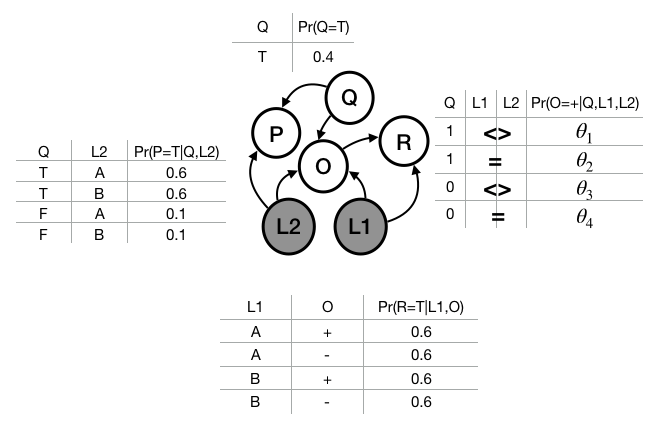
\includegraphics[width=\textwidth]{figs/BN.png}
  \end{minipage}\hfill
  \begin{minipage}[c]{0.45\textwidth}
    \caption{
        \small The model used for generating the datasets. There are four binary random variables, P, Q, O, and R. \textbf{P}: indicates whether or not the employee has high performance; \textbf{Q}: indicates whether or not an employee has high qualification; \textbf{O}: indicates whether or not the colleague submits the positive opinion towards the employee;  \textbf{R}: indicates whether or not the colleague has a positive opinion towards the employee;  \textbf{L1, L2}: indicates the label of the review provider and review receiver (observed).
    } \label{fig:BN}
  \end{minipage}
\end{figure}

We show the effectiveness of FairPSL by performing an empirical evaluation. We investigate two research questions in our experiments:
\begin{description}
\item[Q1] What is the effect of the fairness threshold $\delta$ on the fairness measures $RD/RC/RR$?
\item[Q2] How is decision quality affected by imposing $\delta$-fairness constraints?
\end{description}

Note that although we present the result for specific parameters of the framework in this section, we ran extensive analysis and the results we present are representative. We implemented the MAP inference routines of PSL and FairPSL in Python, using Gurobi-8.1\footnote{\url{www.gurobi.com}} as the backend solver. The FairPSL code, code for the data generator and data is publicly available\footnote{https://github.com/gfarnadi/FairPSL}. 

\subsection{Data generation}
  
We evaluate the FairPSL inference algorithm on synthetic datasets representing the performance review scenario (introduced in Example~\ref{ex:review}). The organization hierarchy is generated synthetically. 
The organization hierarchy generator is parameterized by two numbers: the number of employees in the organization ($n$) and the number of employees managed by each manager ($k$). Each employee is randomly assigned with a label \emph{A} or \emph{B}. An examples organization hierarchy with $n$=50 and $k$=3 is shown in Figure~\ref{fig:hierachy}.

\begin{figure}
  \begin{minipage}[c]{0.3\textwidth}
    \caption{
        \small An example of an organizational hierarchy with five levels and 50 employees with k=3. Each employee either has label A (shown with grey) or B (shown with white).
    }\label{fig:hierachy} 
	\end{minipage} \hfill
    \begin{minipage}[c]{0.7\textwidth}
    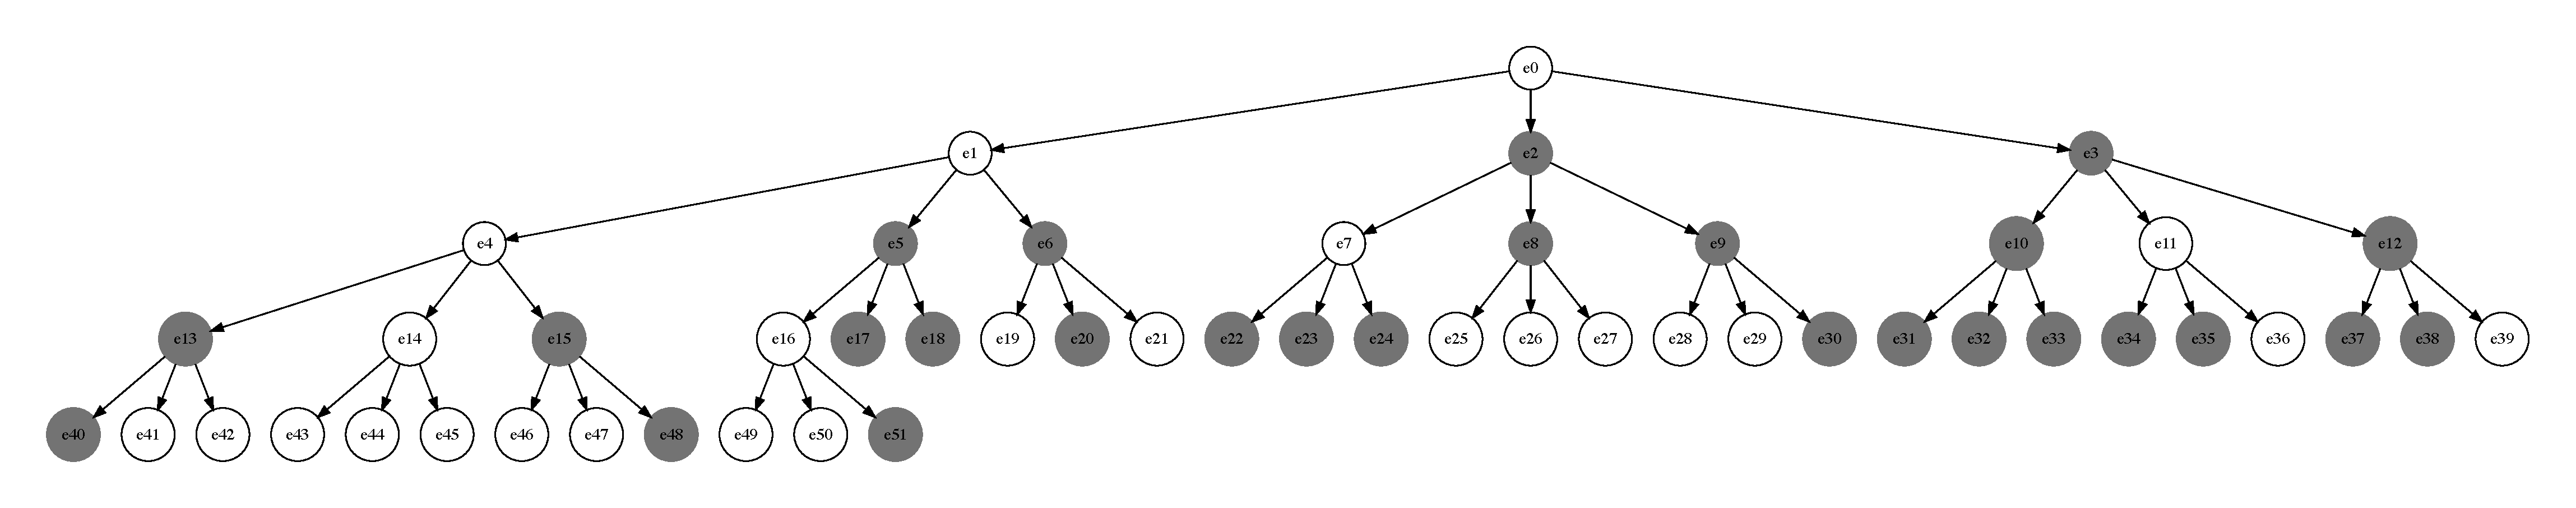
\includegraphics[width=\textwidth]{figs/Uni-hierachy.pdf}
  \end{minipage}
\end{figure}

For each employee, we use the generative model of Figure~\ref{fig:BN} to draw assignments for all the random variables. We assume that only $40\%$ of employees are qualified for promotion and regardless of their labels, employees submit only $60\%$ of their opinions. In addition, due to various personal and environmental factors, only $60\%$ of high quality employees perform well while $10\%$ of low quality employees also perform well regardless of their labels. Note that these numbers are not specific and just chosen for the framework to serve as a representative setting and a proof of concept. The conditional probability table for the opinion variable $O$ is parameterized by four values $(\theta_1, \theta_2, \theta_3, \theta_4)$ which together determine the degree of discrimination against the protected group. Since other parameters in the Bayesian network did not have a direct effect on the degree of discrimination, we fixed them to arbitrary values. 

The results presented in this section are based on an organization hierarchy  with $100$ employees where $k=5$. However, the results of the framework are not sensitive to the settings as we test the framework with various organization sizes ranging from $50$ to $500$ employees and various degree for $k$ ranging from $3$ to $10$. We generated seven datasets given the organization hierarchy using different values for the $\theta$ parameters: $(0.0,1.0,0.0,0.0)$, $(0.33,1.0,0.0,0.0)$, $(0.66,1.0,0.0,0.0)$, $(1.0,1.0,0.0,0.0)$, $(1.0,1.0,0.0,0.33)$, $(1.0,1.0,0.0,0.66)$, $(1.0,1.0,0.0,1.0)$. 
 
In the first three settings the discrimination originates from negative opinions towards qualified outgroup employees. The first setup is an extreme case where the opinion towards outgroup employees is always negative. The discrimination in the last three settings originates from positive opinions towards unqualified ingroup employees. The last setup is an extreme case where the opinion towards ingroup employees is always positive. The fourth setup represent unbiased opinions where employees are treated similarly based on their qualification. 

\paragraph{MAP Inference} We use the model presented in Table~\ref{tab:pslmodel} for MAP inference in PSL and FairPSL (recall that in FairPSL, the $\delta$-fairness constraints corresponding to one of the fairness measures are also added to the model). The observed atoms are $\textit{Manager(m,e)}$, $\textit{PositiveReview(e1,e2)}$ and labels of all employees. The truth values for all other atoms are obtained via MAP inference. We use the truth values obtained for the decision atoms $\textit{ToPromote(e)}$ to compute the fairness measures. We defined the discriminative pattern, and the protected and unprotected groups of this problem in Section~\ref{sec:formulation}.


\subsection{Evaluation results}

\begin{figure}
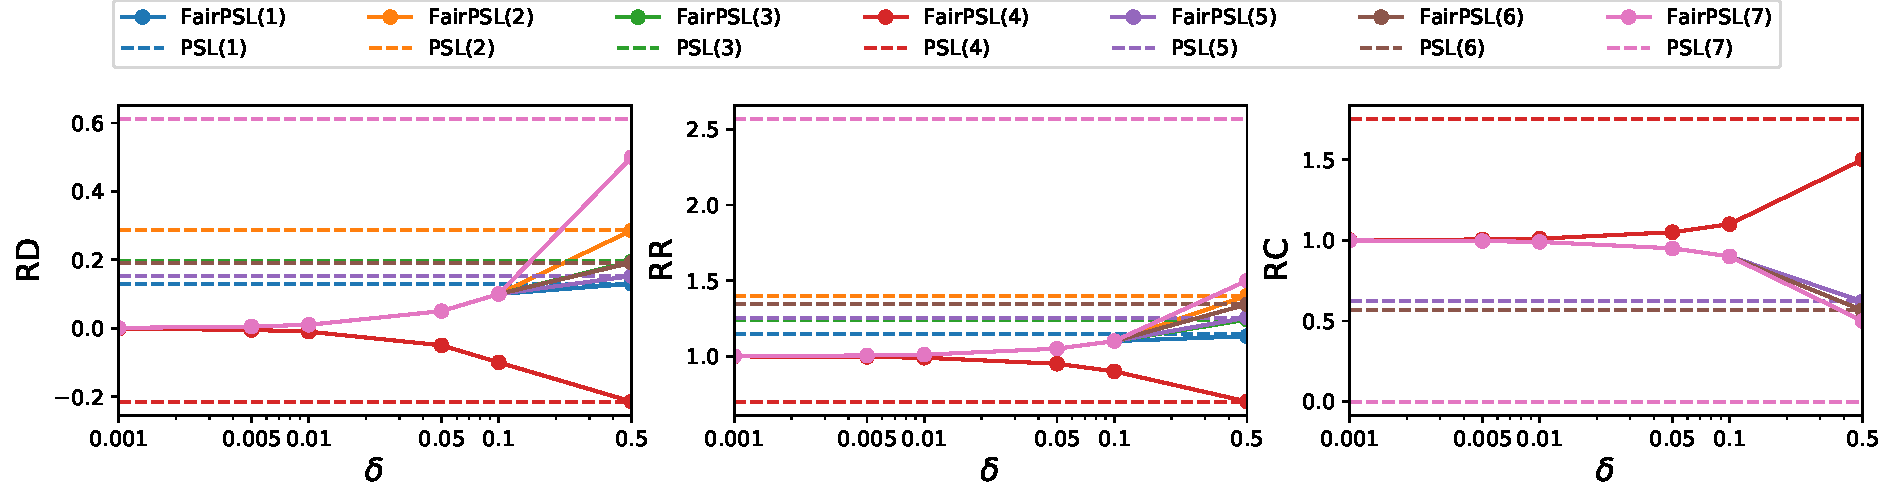
\includegraphics[width=1\linewidth]{figs/results_vis_uni_params.pdf}
\caption{\small Fairness score of predictions obtained by MAP inference of PSL and FairPSL, according to the fairness measures \emph{RD}, \emph{RR}, and \emph{RC}. The labels of datasets are mentioned with parenthesis next to the inference method. The FairPSL values of each measure are obtained by adding the $\delta$-fairness constraint of that measure.\label{fig:results}
}  
\end{figure}

To answer \textbf{Q1}, we run the MAP inference algorithm of PSL and FairPSL on seven synthetic datasets. 
We run the MAP inference of FairPSL multiple times on each dataset: For each of the three fairness measures, we add the corresponding $\delta$-fairness constraint with five thresholds $\{0.001, 0.005, 0.01, 0.05, 0.1, 0.5\}$.

Figure~\ref{fig:results} shows the fairness score of predictions in terms of the three fairness measures. As expected, tighter $\delta$-fairness constraints lead to better scores. Note that the best possible score according to RD is 0, as it computes a difference. Since RR and RC compute ratios, the best possible score according to these measures is 1. In our experiments, with any of these measures, taking $\delta = 0.001$ pushes the score of predictions to its limit.  

The $\delta$-fairness constraints modify the optimization problem of MAP inference by reducing the feasible region to solutions that conform with fairness guarantees. Research question \textbf{Q2} is concerned with the effect of this reduction on the accuracy of predictions. Note that decision quality is the same as the accuracy of predictions. To answer this question, we compare the inferred values for the decision atoms \textit{ToPromote(e)} against their actual values. These values are extracted from the known values of \textit{IsQualified(e)} according to rules 11 and 12 in Table~\ref{tab:pslmodel}. Figure~\ref{fig:accuracy} shows the area under the curve of the receiver operating characteristic~(AUC) of predicting the decision variable in three groups, namely the protected group, the unprotected group (i.e., promotion of the employees who have in-group managers), and all employees. By doing so, we make sure that our fairness constraints do not propagate bias towards either of the populations. Since the results of FairPSL with $\delta$-fairness constraints RR and RC are very similar to the results of RD, we only report the latter here.


\begin{figure}
    \centering
    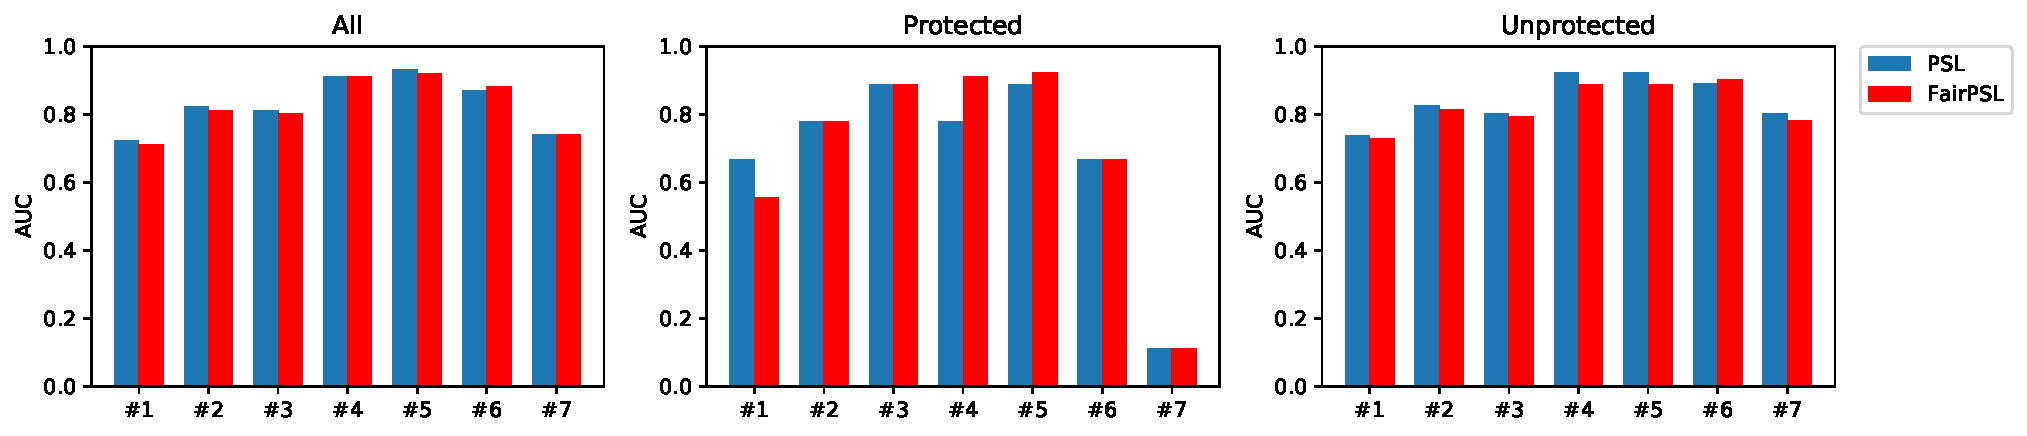
\includegraphics[width=\textwidth]{figs/roc.pdf}
    \caption{\small AUC score of predictions for truth values of unknown atoms \textit{ToPromote(e)} using MAP inference of PSL and FairPSL with $\delta$-fairness constraints $RD$ with $\delta=0.001$.}
    \label{fig:accuracy}
\end{figure}

According to Figure~\ref{fig:accuracy}, the results of both PSL and FairPSL in all seven datasets are close to each other. Note that although fairness may impose a cost in terms of overall accuracy, FairPSL often improves the accuracy of the protected class. Sometimes the overall predictions of FairPSL are even slightly better than PSL (e.g., dataset 6 and 7). As expected, the accuracy of the fourth setting where the opinions are unbiased are similar in both PSL and FairPSL. We observe that prediction of MAP inference for both FairPSL and PSL are similar, thus, in these settings at least, FairPSL guarantees fairness without hurting accuracy. Further investigation is required on the effect of the various ranges of discrimination (i.e., $\theta_1$, $\theta_2$, $\theta_3$, $\theta_4$) on the prediction results of FairPSL.



We also generate various types of organizations in which labels are not uniformly distributed, e.g., one population only occurs at the bottom levels of an organization. While we did not observe any differences in the behavior of our method with respect to accuracy and fairness measure, we found that the degree of discrimination is higher in such organizations. Further investigations on the structure of an organization on discrimination is an interesting direction for future research. 

\section{Conclusion and Future Directions}
\label{sec:conclusion}
Many applications of AI and machine learning affect peoples' lives in important ways. While there is a growing body of work on fairness in AI and ML, it assumes an individualistic notion of fairness.   In this paper, we have proposed a general framework for relational fairness which includes both a rich language for defining discrimination patterns and an efficient algorithm for performing inference subject to fairness constraints. We show our approach enforces fairness guarantees while preserving the accuracy of the predictions. 

There are many avenues for expanding on this work. For example, here we assumed that the discriminative pattern is given, however an automatic mechanism to extract discriminatory situations hidden in a large amount of decision records is an important and required task. Discrimination discovery has been studied for attribute-based fairness~\cite{pedreschi2013discovery}. An interesting next step is discrimination pattern discovery in relational data.

\section*{Acknowledgements}
This work is supported by the National Science Foundation under Grant Numbers CCF-1740850 and IIS-1703331. Golnoosh Farnadi and Behrouz Babaki are  supported by postdoctoral scholarships from IVADO through the Canada First Research Excellence Fund (CFREF) grant.

\begin{thebibliography}{10}
\itemsep=1pt 
\begin{small}

\bibitem{EUlaw}
European union legislation. (a) racial equality directive, 2000; (b) employment
  equality directive, 2000; (c) gender employment directive, 2006; (d) equal
  treatment directive (proposal), 2008.

\bibitem{UKlaw}
{UK} legislation. (a) sex discrimination act, 1975, (b) race relation act,
  1976.

\bibitem{USlaw}
United nations legislation. (a) universal declaration of human rights, 1948,
  (c) convention on the elimination of all forms of racial discrimination,
  1966, (d) convention on the elimination of all forms of discrimination
  against women, 1979.

\bibitem{alshukaili:iswc16}
Duhai Alshukaili, Alvaro A.~A. Fernandes, and Norman~W. Paton.
\newblock Structuring linked data search results using probabilistic soft
  logic.
\newblock In {\em International Semantic Web Conference {(1)}}, volume 9981 of
  {\em Lecture Notes in Computer Science}, pages 3--19, 2016.

\bibitem{bach:jmlr17}
Stephen~H. Bach, Matthias Broecheler, Bert Huang, and Lise Getoor.
\newblock Hinge-loss markov random fields and probabilistic soft logic.
\newblock {\em Journal of Machine Learning Research}, 18:109:1--109:67, 2017.

\bibitem{barocas2016big2}
Solon Barocas and Andrew~D Selbst.
\newblock Big data's disparate impact.
\newblock {\em California Law Review}, 104:671, 2016.

\bibitem{boyd2014networked}
Danah Boyd, Karen Levy, and Alice Marwick.
\newblock The networked nature of algorithmic discrimination.
\newblock In {\em Data and discrimination: Collected essays}, pages 53--57.
  2014.

\bibitem{brewer1979group}
Marilynn~B Brewer.
\newblock In-group bias in the minimal intergroup situation: A
  cognitive-motivational analysis.
\newblock {\em Psychological bulletin}, 86(2):307, 1979.

\bibitem{brewer2007social}
Marilynn~B Brewer.
\newblock The social psychology of intergroup relations: Social categorization,
  ingroup bias, and outgroup prejudice.
\newblock {\em Social Psychology: Handbook of Basic Principles}, 2007.

\bibitem{chouldechova2017fair2}
Alexandra Chouldechova.
\newblock Fair prediction with disparate impact: {A} study of bias in
  recidivism prediction instruments.
\newblock {\em CoRR}, abs/1703.00056, 2017.

\bibitem{dwork2012fairness3}
Cynthia Dwork, Moritz Hardt, Toniann Pitassi, Omer Reingold, and Richard~S.
  Zemel.
\newblock Fairness through awareness.
\newblock In {\em {ITCS}}, pages 214--226. {ACM}, 2012.

\bibitem{ebrahimi:emnlp16}
Javid Ebrahimi, Dejing Dou, and Daniel Lowd.
\newblock Weakly supervised tweet stance classification by relational
  bootstrapping.
\newblock In {\em {EMNLP}}, pages 1012--1017. The Association for Computational
  Linguistics, 2016.

\bibitem{farnadi2018fairness}
Golnoosh Farnadi, Behrouz Babaki, and Lise Getoor.
\newblock Fairness in relational domains.
\newblock In {\em AAAI/ACM Conference on AI, Ethics, and Society (AIES)}, pages
  108--114. ACM, 2018.

\bibitem{feldman2015certifying2}
Michael Feldman, Sorelle~A. Friedler, John Moeller, Carlos Scheidegger, and
  Suresh Venkatasubramanian.
\newblock Certifying and removing disparate impact.
\newblock In {\em {KDD}}, pages 259--268. {ACM}, 2015.

\bibitem{getoor2007introduction}
Lise Getoor and Ben Taskar.
\newblock {\em {Introduction to Statistical Relational Learning}}.
\newblock MIT press Cambridge, 2007.

\bibitem{hardt2016equality3}
Moritz Hardt, Eric Price, and Nati Srebro.
\newblock Equality of opportunity in supervised learning.
\newblock In {\em {NIPS}}, pages 3315--3323, 2016.

\bibitem{kamishima2011fairness}
Toshihiro Kamishima, Shotaro Akaho, and Jun Sakuma.
\newblock Fairness-aware learning through regularization approach.
\newblock In {\em ICDMW}, pages 643--650. {IEEE} Computer Society, 2011.

\bibitem{kouki:recsys15}
Pigi Kouki, Shobeir Fakhraei, James~R. Foulds, Magdalini Eirinaki, and Lise
  Getoor.
\newblock Hyper: {A} flexible and extensible probabilistic framework for hybrid
  recommender systems.
\newblock In {\em RecSys}, pages 99--106. {ACM}, 2015.

\bibitem{counterfactualfairness}
Matt~J. Kusner, Joshua~R. Loftus, Chris Russell, and Ricardo Silva.
\newblock Counterfactual fairness.
\newblock In {\em {NIPS}}, pages 4069--4079, 2017.

\bibitem{Pedreschi:2012}
Dino Pedreschi, Salvatore Ruggieri, and Franco Turini.
\newblock A study of top-k measures for discrimination discovery.
\newblock In {\em {SAC}}, pages 126--131. {ACM}, 2012.

\bibitem{pedreschi2013discovery}
Dino Pedreschi, Salvatore Ruggieri, and Franco Turini.
\newblock The discovery of discrimination.
\newblock In {\em Discrimination and Privacy in the Information Society},
  volume~3 of {\em Studies in Applied Philosophy, Epistemology and Rational
  Ethics}, pages 91--108. Springer, 2013.

\bibitem{ridgeway2004unpacking}
Cecilia~L Ridgeway and Shelley~J Correll.
\newblock Unpacking the gender system: A theoretical perspective on gender
  beliefs and social relations.
\newblock {\em Gender \& society}, 18(4):510--531, 2004.

\bibitem{sridhar:bioinformatics16}
Dhanya Sridhar, Shobeir Fakhraei, and Lise Getoor.
\newblock A probabilistic approach for collective similarity-based drug-drug
  interaction prediction.
\newblock {\em Bioinformatics}, 32(20):3175--3182, 2016.

\bibitem{verma2018fairness2}
Sahil Verma and Julia Rubin.
\newblock Fairness definitions explained.
\newblock In {\em 2018 IEEE/ACM International Workshop on Software Fairness
  (FairWare)}, pages 1--7. IEEE, 2018.

\bibitem{west2014exploiting}
Robert West, Hristo~S. Paskov, Jure Leskovec, and Christopher Potts.
\newblock Exploiting social network structure for person-to-person sentiment
  analysis.
\newblock {\em {TACL}}, 2:297--310, 2014.

\bibitem{zafar2017parity}
Muhammad~Bilal Zafar, Isabel Valera, Manuel Gomez{-}Rodriguez, Krishna~P.
  Gummadi, and Adrian Weller.
\newblock From parity to preference-based notions of fairness in
  classification.
\newblock In {\em {NIPS}}, pages 228--238, 2017.

\bibitem{zemel2013learning}
Richard~S. Zemel, Yu~Wu, Kevin Swersky, Toniann Pitassi, and Cynthia Dwork.
\newblock Learning fair representations.
\newblock In {\em {ICML} {(3)}}, volume~28 of {\em {JMLR} Workshop and
  Conference Proceedings}, pages 325--333. JMLR.org, 2013.

\end{small}
\end{thebibliography}

\end{document}

\end{article}



\begin{article}
{A Human-in-the-loop Perspective on AutoML: Milestones and the Road Ahead}
{Doris Jung-Lin Lee, Stephen Macke, Doris Xin, Angela Lee, Silu Huang, Aditya Parameswaran}
\graphicspath{{submissions/automl/}}
%\documentclass[11pt,dvipdfm]{article}
\documentclass[11pt]{article}
\usepackage{deauthor,times,graphicx} %required
\usepackage{amsmath,amssymb}
\usepackage{multirow}
\usepackage{algorithm}
\usepackage{algpseudocode}
\usepackage{todonotes}
\usepackage{url}

% \graphicspath{{farnadi/}}

\newtheorem{mydef}{\textbf{Definition}}
\newtheorem{myex}{\textbf{Example}}
\newtheorem{mytheorem}{\textbf{Theorem}}


\begin{document}

\title{A Declarative Approach to Fairness in Relational Domains}
\author{Golnoosh Farnadi$^{1,2}$, Behrouz Babaki$^1$, Lise Getoor$^3$\\
$^1$Polytechnique Montr\'{e}al, $^2$ Mila, $^3$ UC Santa Cruz \\
farnadig@mila.quebec, behrouz.babaki@polymtl.ca, getoor@soe.ucsc.edu}

\maketitle

\begin{abstract}
AI and machine learning tools are being used with increasing frequency for decision making in domains that affect peoples' lives such as employment, education, policing and %loan approval
financial qualifications. These uses raise concerns about biases of algorithmic discrimination and have motivated the development of fairness-aware machine learning. However, existing fairness approaches are based solely on attributes of individuals. In many cases, discrimination is much more complex, and taking into account the social, organizational, and other connections between individuals is important. We introduce new notions of fairness that are able to capture the relational structure in a domain. We use first-order logic to provide a flexible and expressive language for specifying complex relational patterns of discrimination. Furthermore, we extend an existing statistical relational learning framework, probabilistic soft logic~(PSL), to incorporate our definition of relational fairness. We refer to this fairness-aware framework FairPSL. FairPSL makes use of the logical definitions of fairnesss but also supports a probabilistic interpretation. In particular, we show how to perform maximum a posteriori~(MAP) inference by exploiting probabilistic dependencies within the domain while avoiding violations of fairness guarantees. Preliminary empirical evaluation shows that we are able to make both accurate and fair decisions.
\end{abstract}

\section{Introduction}
\label{sec:introduction}

Over the past few years, AI and machine learning have become essential components in operations that drive the modern society, e.g., in financial, administrative, and educational spheres. \emph{Discrimination} happens when qualities of individuals which are not relevant to the decision making process influence the decision. Delegating decision making to an automated process raises questions about discriminating against individuals with certain traits based on biases in the data. This is especially important when the decisions have the potential to impact the lives of individuals, for example, the decisions on granting loans, assigning credit, and employment. 

\emph{Fairness} is defined as the absence of discrimination in a decision making process. The goal of \emph{fairness-aware} machine learning is to ensure that the decisions made by an algorithm do not discriminate against a population of individuals~\cite{feldman2015certifying2,boyd2014networked,hardt2016equality3}. Fairness has been well studied in the social sciences and legal scholarship (for an in-depth review see~\cite{barocas2016big2}), and there is emerging work on fairness-aware ML within the AI and computer science communities. For example, fairness through awareness/Lipschitz property~\cite{dwork2012fairness3}, individual fairness~\cite{zemel2013learning}, statistical parity/group fairness~\cite{kamishima2011fairness}, counterfactual fairness~\cite{counterfactualfairness}, demographic parity/disparate impact~\cite{feldman2015certifying2,chouldechova2017fair2}, preference-based fairness~\cite{zafar2017parity}, and equality of opportunity~\cite{hardt2016equality3}.

The existing work in fairness-aware machine learning is based on a definition of discrimination where a decision is influenced by an \emph{attribute} of an individual. An attribute value upon which discrimination is based (such as gender, race, or religion) is called a \emph{sensitive attribute}. The sensitive attribute defines a population of vulnerable individuals known as the \emph{protected group}. A fair decision-making process treats the protected group the same as the \emph{unprotected group}. 

However, in many social contexts, discrimination is the result of complex interactions and can not be described solely in terms of attributes of an individual. For example, consider an imaginary scenario in an organization in which younger female workers who have older male supervisors have lower chances of promotion than their male counterparts.\footnote{Of course, many other patterns may be possible: female bosses may promote female subordinates and discriminate against male workers, or male bosses may promote female employees.  Our goal is to provide a general framework which is able to describe arbitrarily complex discrimination patterns.} 
 This discrimination pattern involves two attributes of the individual (gender and age), a relationship with another individual (supervisor), and two attributes of the second individual. Addressing such complex cases poses two challenges. First, the concepts of discrimination and fairness need to be extended to capture not only attributes of individuals but also the relationships between them. Second, a process is required that ensures that fair decisions are made about individuals who are affected by such patterns. In this paper we address both of these challenges.
We use first-order logic (FOL) to extend the notion of fairness to the relational setting. FOL is an expressive representation for relational problems which is also widely used for learning in relational domains. Moreover, we extend an existing framework for statistical relational learning~\cite{getoor2007introduction} called probabilistic soft logic (PSL)\footnote{http://psl.linqs.org/}~\cite{bach:jmlr17}. PSL combines logic and probability for learning and reasoning over uncertain relational domains. One of the most common reasoning tasks in PSL is called maximum a posteriori (MAP) inference, which is performed by finding the most probable truth values for unknowns over a set of given evidence. We develop a new MAP inference algorithm which is able to maximize the a posteriori values of unknown variables \emph{subject to} fairness guarantees. An early version of this paper which this work builds upon and extends appeared in~\cite{farnadi2018fairness}.

\looseness-1
Our contributions are as follows: 1) we propose fairness-aware machine learning for the relational setting; 2) we extend PSL into a fairness-aware framework called FairPSL which can represent the logical definition of fairness; 3) we develop a new MAP inference algorithm which is able to maximize the posteriori values of unknown variables \emph{subject to} fairness guarantees; 4) we empirically evaluate our proposed framework on synthetic data. 

\section{Motivation}
\label{sec:motivation}

Discrimination in social contexts have been studied in the field of social psychology~\cite{brewer2007social,brewer1979group,ridgeway2004unpacking}. There is a large literature on various aspects of relational bias in social contexts such as \emph{in-group-out-group bias}, \emph{gender bias}, and \emph{ethnicity-based favoritism} that can result in discrimination. 
As an example, consider gender bias in the workplace that reflects stereotypically masculine criteria and male-based favoritism. Such gender bias 
typically places women in lower positions and negatively impacts their opportunities. Further, lack of women in leadership positions may affect the promotion of women and results in a glass ceiling that keeps women from rising beyond a certain level in the hierarchy. This scenario shows that considering  protected attributes such as gender is not always sufficient to detect the source of bias and avoid discrimination, one also has to consider the relational information, in this case the organization hierarchy. Note that this can be generalized to any ingroup/outgroup scenario where the sensitive attribute could be race, religion, age, marital-status, etc.

The existing work on designing fair algorithms in machine learning exclusively focuses on \emph{attribute-based fairness}, which is based on the following assumptions: First, there is an assumption that the individuals (sometimes referred to as units or entities) are independent and described by simple attribute vectors. Second, the group for which one wishes to ensure fairness (known as the \emph{protected group}) is defined on the basis of some attribute values. Finally, there is a decision that is associated with each individual, and the goal is to ensure that members of the protected group are subject to a fair decision (we discuss different fairness measures in Section~\ref{sec:fairnessmeasure}).  We illustrate  attribute-based fairness in the following example. 

\begin{myex}[Loan Processing]
\label{ex:loan}
A bank bases its decisions about granting a loan on attributes of the applicant. The goal is to decide whether to grant a loan to an applicant using a predictive model. The bank needs to ensure that the obey fair lending practices and ensure that gender, race, sexual orientation of applicants has no influence on the decision. In this scenario, the protected group is the historically disadvantaged applicants.  
\end{myex}
The current fairness-aware machine learning techniques are not capable of modeling relations and hence cannot be used to make the decision making model fair. However, in many decision making scenarios, especially in social and organizational settings, the domain is relational, and the protected group itself might be best represented using a relational definition. We illustrate this setting in the following scenario:
\begin{myex}[Performance Review]
\label{ex:review}
Consider an organization where decisions about the promotion of employees is based on two criteria: 1) an objective performance measure, and 2) the opinion of their direct and indirect managers above them. The opinions are inferred from the performance reviews which are collected periodically. Not every manager can submit a review for all its subordinates, this is especially the case for top-level managers who have a large number of subordinates. Hence, the opinions of managers are collectively inferred from the opinions of their sub-ordinates. However, some employees may be biased, and judge other employees unfavorably, by favoring employees who are similar to themselves (same gender, race, religion, etc.) over employees who are dissimilar. The organization needs to ensure that promotion of employees do not have any relational bias caused by in-group-out-group favoritism.

\end{myex}
Example~\ref{ex:review} describes a prediction problem over a database that consists of relations between employees. Such prediction tasks are best handled by techniques from the relational learning domain. To ensure fair prediction in such settings, we need to extend the notion of \emph{attribute-based fairness} to \emph{relational fairness}. Throughout this paper, we use the performance review problem as a running example for relational fairness.

\section{Fairness Formalism}
\label{sec:formulation}

A representation that can describe different types of entities and different relationships between them is called relational. In this section, we use first-order logic to define relational fairness. We employ first-order logic as an expressive representation formalism which can represent objects and complex relationships between them. We start by defining an atom:

\begin{mydef}[Atom]
An atom is an expression of the form $P(a_1, a_2, \ldots, a_n)$ where each argument $a_1, a_2,$ $\ldots,$ $a_n$ is either a constant or a variable. The finite set of all possible substitutions of a variable to a constant for a particular variable $a$ is called its \textit{domain} $D_{a}$. If all variables in $P(a_1, a_2, \ldots, a_n)$ are substituted by some constant from their respective domain, then we call the resulting atom a \textit{ground atom}. 
\end{mydef}

\begin{myex}
In our loan processing problem (Example~\ref{ex:loan}), we can represent applicants' attributes by atoms. For instance, atom $Female(v)$ indicates whether or not applicant $v$ is female. Similarly, we can represent relations with atoms. In the performance review problem in Example~\ref{ex:review} the atom $Manager(m,e)$ indicates whether or not employee $m$ is a direct or indirect manager of employee $e$.
\end{myex}

The relational setting provides the flexibility to express complex definitions with formulae.

\begin{mydef}[Formula] 
A formula is defined by induction: every atom is a formula. If $\alpha$ and $\beta$ are formulae, then $\alpha \vee \beta$, $\alpha \wedge \beta$, $\neg \alpha$, $\alpha \rightarrow \beta$ are formulae. If $x$ is a variable and $\alpha$ is a formula, then the quantified expressions of the form $\exists x$ $\alpha$ and $\forall x$ $\alpha$ are formulae.    
\end{mydef}

To characterize groups of individuals based on a formula, we define the notion of \emph{population}.

\begin{mydef}[Population]
We denote formula $F$ which has only one free variable $v$ (i.e., other variables in $F$ are quantified) by $F[v]$. The population defined by $F[v]$ is the set of substitutions of $v$ for which $F[v]$ holds.   
\end{mydef}


\begin{myex}
\label{ex:disformula}
Consider the formula $F[v] := \forall u, \, \textit{Manager}(u,v) \rightarrow \neg \textit{SameGroup}(u, v)$. The population specified by this formula is the set of individuals all of whose managers belong to a group different from theirs. 
\end{myex}

The truth value of a formula is derived from the truth value of atoms that it comprises, according to the rules of logic. Each possible assignment of truth values to ground atoms is called an \emph{interpretation}. 


\begin{mydef}[Interpretation]
An interpretation $I$ is a mapping that associates a truth value $I(P)$ to each ground atom $P$. For Boolean truth values, $I$ associates true to 1 and false to 0 truth values. For soft logic (see Definition~\ref{def:softlogic}) $I$ maps each ground atom $P$ to a truth value in interval $[0, 1]$.
\end{mydef}

In attribute-based fairness, it is assumed that there is a certain attribute of individuals, i.e, the sensitive attribute,  that we do not want to affect a decision. Gender, race, religion and marital status are examples of sensitive attributes. Discrimination has been defined in social science studies as a treatment in favor or against a group of individuals given their sensitive attribute. This group of individuals is the protected group. 

In a relational setting, both the sensitive attributes of an individual and their participation in various relations may have an undesired effect on the final decision. We characterize the protected group in a relational setting by means of a population. In practice, we are often interested in maintaining fairness for a specific population such as applicants, students, employees, etc. This population is then partitioned into the protected and unprotected groups. We define a \emph{discriminative pattern} which is a pair of formulae to capture these groups: 1) $F_1[v]$: to specify the difference between the protected and unprotected groups and 2) $F_2[v]$: to specify the population over which we want to maintain fairness. 

\begin{mydef}[Discriminative pattern]
A discriminative pattern is a pair $\textit{DP}[v]:=(F_1[v], F_2[v])$ , where $F_1[v]$ and $F_2[v]$ are formulae.
\end{mydef}

\begin{myex}
\label{ex:pattern}
The two formulae in the discrimination pattern $\textit{DP}[v]:= \big((\forall u, \,  \textit{Manager}(u,v) \rightarrow  \neg \textit{SameGroup}(u, v)),$ $\textit{Employee}(v)\big)$ specify two populations, namely all employees and those employees who belong to a group different from their managers.
\end{myex}

Given the definition of the discriminative pattern, we have a rich language to define the scope of the protected and unprotected groups in a relational setting.

\begin{mydef}[Protected group] Given an interpretation $I$, the protected group is a population of the form:
{$$PG :=\{ v : F_1[v] \wedge F_2[v]\}$$}
which is defined as the set of all instances hold for variable $v$ for which $F_1[v] \wedge F_2[v]$ is true under interpretation $I$, that is, $I(F_1[v] \wedge F_2[v]) = 1$. 
Similarly, the \emph{unprotected group} is a population of the form: 
{$$UG := \{ v : \neg F_1[v] \wedge  F_2[v]\}$$}
which is defined as the set of all instances hold for variable $v$ 
for which $I(\neg F_1[v] \wedge F_2[v]) = 1$. 
\end{mydef}

\begin{myex}
The protected group of the discrimination pattern specified in Example~\ref{ex:pattern} is {$PG := \big\{ v : \big(\forall u, \,$ $ \textit{Manager}(u, v) \rightarrow \neg \textit{SameGroup}(u, v)\big) \wedge \textit{Employee}(v) \big\}$} and the unprotected group is {$UG :=  \big\{ v:  \big(\exists u, \, \textit{Manager}(u,v) \wedge \textit{SameGroup}(u, v)\big) \wedge \textit{Employee}(v) \big\}$}. This means our protected group is the set of employees belonging to a group different from their managers,
and our unprotected group consists of other employees. 
\end{myex}

Discrimination is defined in terms of a treatment or decision that distinguishes between the protected and unprotected groups. Here we define the \emph{decision} atom.
\begin{mydef}[Decision atom] A decision atom $d(v)$ is an atom containing exactly one variable $v$ that specifies a decision affecting the protected group which is defined either by law or end-user.
\end{mydef}
\begin{myex}
The decision atom ${\textit ToPromote}(v)$ indicates whether or not $v$ receives a promotion.
\end{myex}

Note that the fairness formulation in this section is designed for the relational setting, however relational fairness subsumes the attribute-based fairness such that: a sensitive attribute is defined by an atom with one argument and $F_2[v]$ in discrimination pattern is $\textit{Applicant}(v)$. For example, discrimination pattern of our loan processing problem in Example~\ref{ex:loan} is of the form $\textit{DP} := ( \textit{Female}(v), \textit{Applicant}(v))$ that denotes female applicants as the protected group (i.e., $PG :=  \{ v: \textit{Female}(v) \}$) and male applicants as the unprotected group (i.e., $UG := \{ v: \neg \textit{Female}(v)\}$).


\section{Fairness Measures}
\label{sec:fairnessmeasure}

Over the past few years, many fairness measures have been introduced~\cite{verma2018fairness2}. An important class of these measures are \emph{group fairness} measures which quantify the inequality between different subgroups. Some of the most popular measures in this class include \emph{equal opportunity}, \emph{equalized odds}, and \emph{demographic parity}~\cite{hardt2016equality3}. In this paper we restrict our focus to the latter. In an attribute-value setting, demographic parity means that the decision should be independent of the protected attributes. Assume that binary variables $A$ and $C$ denote the decision and protected attributes, and the preferred value of $A$ is one. Demographic parity requires that:

\begin{equation*}
    P(A=1 | C=0) = P(A=1 | C=1)
\end{equation*}

We will now generalize this measure to the relational setting using the notations defined in Section~\ref{sec:formulation}. Let $a$ and $c$ denote the counts of denial (i.e., negative decisions) for protected and unprotected groups, and $n_{1}$ and $n_{2}$ denote their sizes, respectively. Given the decision atom $d(v)$, discriminative pattern $\textit{DP}(F_1[v], F_2[v])$, and interpretation $I$, these counts are computed by the following equations: 
{
\begin{flalign}
    & a \equiv \sum_{v \in D_v} I\big( \neg d(v) \wedge  F_1[v] \wedge F_2[v]) \label{eq:a}\\
    & c \equiv \sum_{v \in D_v} I\big( \neg d(v) \wedge  \neg F_1[v] \wedge  F_2[v]) \label{eq:c}\\
    & n_{1} \equiv \sum_{v \in D_v} I\big(F_1[v] \wedge F_2[v]) \label{eq:n1}\\
    & n_{2} \equiv \sum_{v \in D_v} I\big(\neg F_1[v] \wedge  F_2[v]) \label{eq:n2}
\end{flalign}}
The proportions of denying for protected and unprotected groups are $p_1 = \frac{a}{n_1}$ and $p_2 = \frac{c}{n_2}$, respectively. There are a number of data-driven measures~\cite{Pedreschi:2012} which quantify demographic disparity and can be defined in terms of $p_1$ and $p_2$:
\begin{itemize}
    \item \textbf{Risk difference}: $RD = p_1 - p_2$, also known as absolute risk reduction. 
    \item \textbf{Risk Ratio}: $RR = \frac{p_1}{p_2}$, also known as relative risk. 
    \item \textbf{Relative Chance}: $RC = \frac{1 - p_1}{1 - p_2}$ also, known as selection rate.
\end{itemize}
These measures have been used in the legal systems of European Union, UK, and US~\cite{EUlaw,UKlaw,USlaw}. Notice that RR is the ratio of the proportion of benefit denial between the protected and unprotected groups, while RC is the ratio of the proportion of benefit granted. Finally, we introduce the notion of $\delta$-fairness.

\begin{mydef}[$\delta$-fairness]
If a fairness measure for a decision making process falls within some $\delta$-window, then the process is \emph{$\delta\text{-fair}$}. Given $0 \leq \delta \leq 1$, the  $\delta$-windows for measures RD/RR/RC are defined as:
{\begin{flalign*}
	     - \delta \leq &RD \leq \delta \\
	     1- \delta \leq &RR \leq 1+ \delta\\
	     1- \delta \leq &RC \leq 1+ \delta
	\end{flalign*}}
\end{mydef}

To overcome the limitations of attribute-based fairness, we introduce a new statistical relational learning~(SRL) framework~\cite{getoor2007introduction} suitable for modelling fairness in relational domain. In the next section, we review probabilistic soft logic~(PSL). We then extend PSL with the definition of relational fairness introduced above in Section~\ref{sec:fairMAP}. Our fairness-aware framework, ``FairPSL'', is the first SRL framework that performs fair inference. 

\section{Background: Probabilistic Soft Logic}
\label{sec:psl}

In this section, we review the syntax and semantics of PSL, and in the next section we extend MAP inference in PSL with fairness constraints to define MAP inference in FairPSL.

PSL is a probabilistic programming language for defining hinge-loss Markov random fields~\cite{bach:jmlr17}. Unlike other SRL frameworks whose atoms are Boolean, atoms in PSL can take continuous values in the interval $[0,1]$. PSL is an expressive modeling language that can incorporate domain knowledge with first-order logical rules and has been used successfully in various domains, including bioinformatics~\cite{sridhar:bioinformatics16}, recommender systems~\cite{kouki:recsys15}, natural language processing~\cite{ebrahimi:emnlp16}, information retrieval~\cite{alshukaili:iswc16}, and social network analysis~\cite{west2014exploiting}, among many others. 
 
A PSL model is defined by a set of first-order logical rules called \emph{PSL rules}.

\begin{mydef} [PSL rule] a PSL rule $r$ is an expression of the form:
{\begin{equation}
\lambda_{r}: T_1 \land T_2 \land \ldots \land T_w \rightarrow H_1 \vee H_2 \vee \ldots \vee H_l
\end{equation}}

where { $T_1, T_2, \ldots, T_w, H_1, H_2, \ldots, H_l$} are atoms or negated atoms and { $\lambda_{r} \in \mathbb{R}^{+} \cup \infty$} is the weight of the rule $r$.  We call { $T_1 \land T_2 \land \ldots \land T_w$} the body of $r$ ($r_{body}$), and { $H_1 \vee H_2 \vee \ldots \vee H_l$} the head of $r$ ($r_{head}$).
\end{mydef}


Since atoms in PSL take on continuous values in the unit interval $[0,1]$, next we define soft logic to calculate the value of the PSL rules under an interpretation $I$.

\begin{mydef}[Soft logic]
\label{def:softlogic}
The ({$\tilde{\wedge}$}) and ({$\tilde{\vee}$}) and negation ({$\tilde{\neg}$}) are defined as follows. For {$m, n \in [0,1]$} we have: {$m \tilde{\wedge} n = \max(m+n -1, 0)$}, {$m \tilde{\vee} n = \min(m+n , 1)$} and {$\tilde{\neg} m = 1 - m$}. The $\, \tilde{} \,$ indicates the relaxation over Boolean values.
\end{mydef}

The probability of truth value assignments in PSL is determined by the rules' \emph{distance to satisfaction}.

\begin{mydef}[The distance to satisfaction]
The distance to satisfaction $d_{r}(I)$ of a rule $r$ under an interpretation $I$ is defined as:
{
\begin{equation}
d_{r}(I) = \max\{0, I(r_{body})-I(r_{head})\}
\end{equation}}
\end{mydef}

By using Definition~\ref{def:softlogic}, one can show that the closer the interpretation of a grounded rule $r$ is to 1, the smaller its distance to satisfaction. A PSL model induces a distribution over interpretations $I$. Let $R$ be the set of all grounded rules, then the probability density function is:
{
\begin{equation}
f(I) ={\frac{1}{Z}} \exp[-\sum_{r\in R} \lambda_{r}(d_{r}(I))^p]
\label{eq:potential}
\end{equation}
}
\noindent where { $\lambda_{r}$} is the weight of rule $r$, {
$Z = \int_{I} \exp[ -\sum_{r\in R} \lambda_{r}(d_{r}(I))^p]$
} is a normalization constant, and { $p \in \{1,2\}$} provides a choice of two different loss functions, $p=1$ (i.e., linear), and $p=2$ (i.e, quadratic). These probabilistic models are instances of hinge-loss Markov random fields~(HL-MRF)~\cite{bach:jmlr17}. The goal of maximum a posteriori (MAP) inference is to find the most probable truth assignments $I_{\textit{MPE}}$ of unknown ground atoms given the evidence which is defined by the interpretation $I$. Let $X$ be all the evidence, i.e., $X$ is the set of ground atoms such that $\forall x \in X, I(x)$ is known, and let $Y$ be the set of ground atoms such that $\forall y \in Y, I(y)$ is unknown. Then we have
{
\begin{equation}
I_{\textit{MAP}}(Y) = \textit{arg}\max_{I(Y)} P(I(Y)|I(X))
\end{equation}}
Maximizing the density function in Equation~\ref{eq:potential} is equivalent to minimizing the weighted sum of the distances to satisfaction of all rules in PSL. 

\begin{table*}[t]
    \centering
    \begin{tabular}{|lll|}
    \hline
    &&\\
    $R1$ & $\lambda_1$ &: $\textit{IsQualified}(e) \rightarrow \textit{HighPerformance}(e)$ \\
    $R2$ & $\lambda_1$ &: $\neg \textit{IsQualified}(e) \rightarrow \neg \textit{HighPerformance}(e)$ \\
    $R3$ & $\infty$ &: $\textit{PositiveReview}(e1, e2) \rightarrow \textit{PositiveOpinion}(e1, e2)$ \\
    $R4$ & $\infty$ &: $\neg \textit{PositiveReview}(e1, e2) \rightarrow \neg \textit{PositiveOpinion}(e1, e2)$ \\
    $R5$ & $\lambda_1$ &: $\textit{PositiveOpinion}(e1, e2) \wedge \textit{Manager}(m, e1) \rightarrow \textit{PositiveOpinion}(m, e2)$ \\
    $R6$ & $\lambda_1$ &: $\neg \textit{PositiveOpinion}(e1, e2) \wedge \textit{Manager}(m, e1) \rightarrow \neg \textit{PositiveOpinion}(m, e2)$ \\
    $R7$ & $\lambda_1$ &: $\textit{PositiveOpinion}(m, e) \wedge \textit{Manager}(m, e) \rightarrow \textit{IsQualified}(e)$ \\
    $R8$ & $\lambda_1$ &: $\neg \textit{PositiveOpinion}(m, e) \wedge \textit{Manager}(m, e) \rightarrow \neg \textit{IsQualified}(e)$ \\
    $R9$ &  $\lambda_1$ &: $\neg \textit{ToPromote}(e)$\\
    $R10$ & $\infty$ &: $\textit{IsQualified}(e) \rightarrow \textit{ToPromote}(e)$ \\
    $R11$ & $\infty$ &: $\neg \textit{IsQualified}(e) \rightarrow \neg \textit{ToPromote}(e)$ \\
    &&\\
    \hline
    \end{tabular}
    \caption{\small A simplified PSL model for the \emph{Performance Reviewing} problem}
    \label{tab:pslmodel}
\end{table*}

\begin{myex}
\label{ex:pslmodel}
The simplified PSL model for the performance reviewing problem in Example\ref{ex:review} is given in Table~\ref{tab:pslmodel}. The goal of MAP inference for this problem is to infer employees to promote. We simplified the model by assigning the same weight to all soft rules (i.e., $\lambda_i= 1$ where $i=\{1,2,5,6,7,8,9\}$). Below we explain the meaning of each rule in the model.

Rule $R1$ indicates that qualified employees have high performance and similarly rule $R2$ expresses that a negative qualification of employees is derived from their low performance. Rules $R5$ and $R6$ presents the propagation of opinion from bottom to top of the organizational hierarchy, i.e., managers have similar opinions towards employees given the opinions of their sub-ordinate managers. And rules $R7$ and $R8$ indicate that the positive/negative opinion of direct/indirect managers derive from the qualification of an employee. Rule $R9$ indicates the prior that not all employees get promoted. We also have four hard constraints (i.e., rules $R3$, $R4$, $R10$ and $R11$) where the weight of the rules are $\infty$. Rules $R3$ and $R4$ indicate that submitted positive/negative reviews should reflect positive/negative opinions. And two rules $R10$ and $R11$ show that a highly qualified employee should get promoted. 
\end{myex}

\section{Fairness-aware PSL (FairPSL)}
\label{sec:fairMAP}

The standard MAP inference in PSL aims at finding values that maximize the conditional probability of unknowns. Once a decision is made according to these values, one can use the fairness measure to quantify the degree of discrimination. A simple way to incorporate fairness in MAP inference is to add the $\delta$-fairness constraints to the corresponding optimization problem.   

Consider risk difference, $\textit{RD}$, where $\textit{RD} \equiv \frac{\mathbf{a}}{n_1} - \frac{\mathbf{c}}{n_2}$. The $\delta$-fairness constraint $-\delta \leq \textit{RD} \leq \delta$ can be encoded as the following constraints:
{\begin{align}
    & n_2 \mathbf{a} - n_1 \mathbf{c} - n_1 n_2 \delta \leq 0 \label{eq:RD1}\\
    & n_2 \mathbf{a} - n_1 \mathbf{c} + n_1 n_2 \delta \geq 0
\end{align}}
Similarly, from $\textit{RR} \equiv \frac{\mathbf{a} / n_1}{\mathbf{c} / n_2}$ and the $\delta$-fairness constraint $1 - \delta \leq \textit{RR} \leq 1 + \delta$ we obtain:
{\begin{align}
    & n_2 \mathbf{a} - (1 + \delta) n_1 \mathbf{c} \leq 0 \\
    & n_2 \mathbf{a} - (1 - \delta) n_1 \mathbf{c} \geq 0
\end{align}}
And finally, $\textit{RC} \equiv \frac{1 - \mathbf{a} / n_1}{1 - \mathbf{c} / n_2}$ and the $\delta$-fairness constraint $1 - \delta \leq \textit{RC} \leq 1 + \delta$ gives:
{ \begin{align}
    & - n_2 \mathbf{a} + (1 + \delta) n_1 \mathbf{c} - \delta n_1 n_2 \leq 0 \\
    & - n_2 \mathbf{a} + (1 - \delta) n_1 \mathbf{c} + \delta n_1 n_2 \geq 0 \label{eq:RC2}
\end{align}}
A primary advantage of PSL over similar frameworks is that its MAP inference task reduces to a convex optimization problem which can be solved in polynomial time. To preserve this advantage, we need to ensure that the problem will remain convex after the addition of $\delta$-fairness constraints. 

\begin{mytheorem}
The following condition is sufficient for preserving the convexity of MAP inference problem after addition of $\delta$-fairness constraints: The formulae $F_1[v]$ and $F_2[v]$ do not contain an atom $y \in Y$ and all atoms in $F_1[v]$ and $F_2[v]$ have values zero or one.
\end{mytheorem}
\begin{proof}
Since $I(F_1[v])$ and $I(F_2[v])$ do not depend on $I(Y)$, the values $n_{1}$ and $n_{2}$ are constants that can be computed in advance. Let us define the sets $D_v^a = \{ v \in D_v : F_1[v] \wedge F_2[v] \, \text{is true} \}$ and $D_v^c = \{ v \in D_v : \neg F_1[v] \wedge F_2[v] \, \text{is true} \}$. Since $F_1[v]$ and $F_2[v]$ can be only zero or one, we can rewrite the equations~\ref{eq:a} and \ref{eq:c} as:
{
\begin{align*}
    & \mathbf{a} = \sum_{v \in D_v^a} I(\neg d(v)) = |D_v^a| - \sum_{v \in D_v^a} I(d(v))\\
    & \mathbf{c} = \sum_{v \in D_v^c} I(\neg d(v)) = |D_v^c| - \sum_{v \in D_v^c} I(d(v))
\end{align*}}
\noindent which indicates that $\mathbf{a}$ and $\mathbf{c}$ can be expressed as linear combinations of variables in the optimization problem. This means that constraints~\ref{eq:RD1}-\ref{eq:RC2} are linear. Hence, addition of these constraints preserves the convexity of the optimization problem. 
\end{proof}

\section{Experiments}
\label{sec:experiment}

\begin{figure}
  \begin{minipage}[c]{0.6\textwidth}
    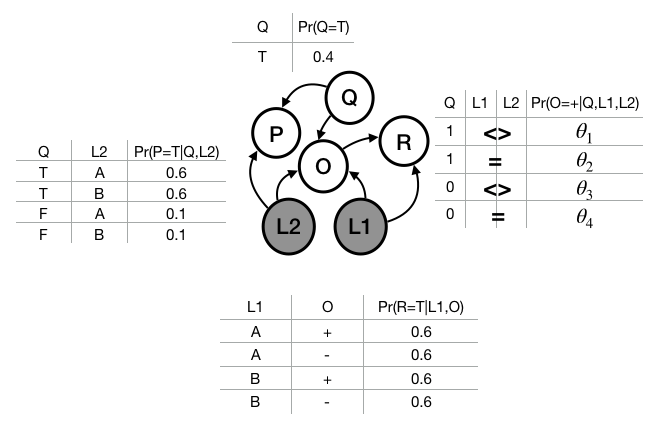
\includegraphics[width=\textwidth]{figs/BN.png}
  \end{minipage}\hfill
  \begin{minipage}[c]{0.45\textwidth}
    \caption{
        \small The model used for generating the datasets. There are four binary random variables, P, Q, O, and R. \textbf{P}: indicates whether or not the employee has high performance; \textbf{Q}: indicates whether or not an employee has high qualification; \textbf{O}: indicates whether or not the colleague submits the positive opinion towards the employee;  \textbf{R}: indicates whether or not the colleague has a positive opinion towards the employee;  \textbf{L1, L2}: indicates the label of the review provider and review receiver (observed).
    } \label{fig:BN}
  \end{minipage}
\end{figure}

We show the effectiveness of FairPSL by performing an empirical evaluation. We investigate two research questions in our experiments:
\begin{description}
\item[Q1] What is the effect of the fairness threshold $\delta$ on the fairness measures $RD/RC/RR$?
\item[Q2] How is decision quality affected by imposing $\delta$-fairness constraints?
\end{description}

Note that although we present the result for specific parameters of the framework in this section, we ran extensive analysis and the results we present are representative. We implemented the MAP inference routines of PSL and FairPSL in Python, using Gurobi-8.1\footnote{\url{www.gurobi.com}} as the backend solver. The FairPSL code, code for the data generator and data is publicly available\footnote{https://github.com/gfarnadi/FairPSL}. 

\subsection{Data generation}
  
We evaluate the FairPSL inference algorithm on synthetic datasets representing the performance review scenario (introduced in Example~\ref{ex:review}). The organization hierarchy is generated synthetically. 
The organization hierarchy generator is parameterized by two numbers: the number of employees in the organization ($n$) and the number of employees managed by each manager ($k$). Each employee is randomly assigned with a label \emph{A} or \emph{B}. An examples organization hierarchy with $n$=50 and $k$=3 is shown in Figure~\ref{fig:hierachy}.

\begin{figure}
  \begin{minipage}[c]{0.3\textwidth}
    \caption{
        \small An example of an organizational hierarchy with five levels and 50 employees with k=3. Each employee either has label A (shown with grey) or B (shown with white).
    }\label{fig:hierachy} 
	\end{minipage} \hfill
    \begin{minipage}[c]{0.7\textwidth}
    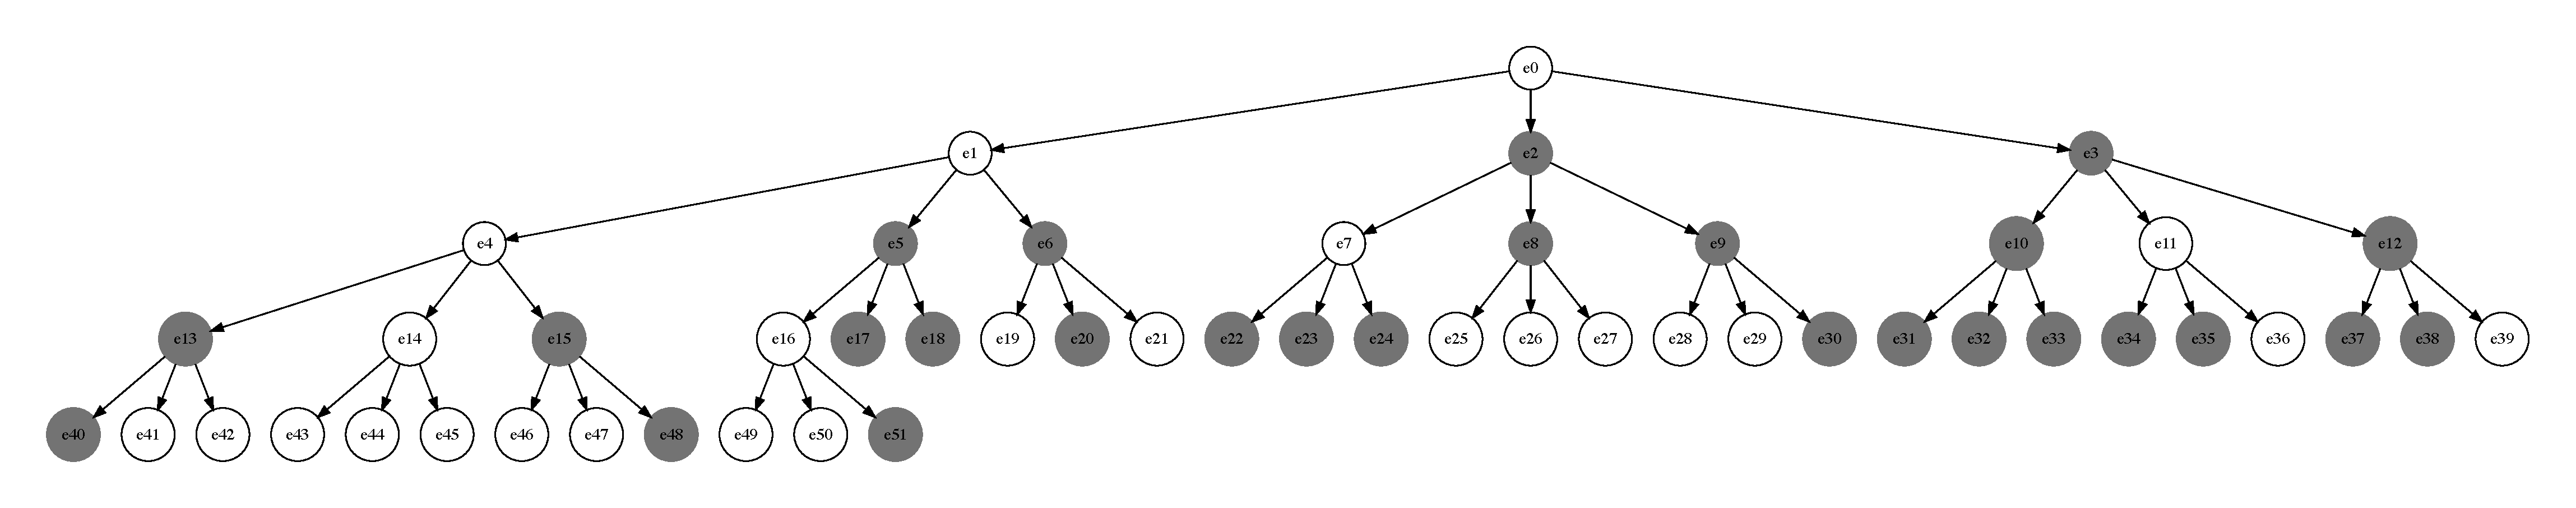
\includegraphics[width=\textwidth]{figs/Uni-hierachy.pdf}
  \end{minipage}
\end{figure}

For each employee, we use the generative model of Figure~\ref{fig:BN} to draw assignments for all the random variables. We assume that only $40\%$ of employees are qualified for promotion and regardless of their labels, employees submit only $60\%$ of their opinions. In addition, due to various personal and environmental factors, only $60\%$ of high quality employees perform well while $10\%$ of low quality employees also perform well regardless of their labels. Note that these numbers are not specific and just chosen for the framework to serve as a representative setting and a proof of concept. The conditional probability table for the opinion variable $O$ is parameterized by four values $(\theta_1, \theta_2, \theta_3, \theta_4)$ which together determine the degree of discrimination against the protected group. Since other parameters in the Bayesian network did not have a direct effect on the degree of discrimination, we fixed them to arbitrary values. 

The results presented in this section are based on an organization hierarchy  with $100$ employees where $k=5$. However, the results of the framework are not sensitive to the settings as we test the framework with various organization sizes ranging from $50$ to $500$ employees and various degree for $k$ ranging from $3$ to $10$. We generated seven datasets given the organization hierarchy using different values for the $\theta$ parameters: $(0.0,1.0,0.0,0.0)$, $(0.33,1.0,0.0,0.0)$, $(0.66,1.0,0.0,0.0)$, $(1.0,1.0,0.0,0.0)$, $(1.0,1.0,0.0,0.33)$, $(1.0,1.0,0.0,0.66)$, $(1.0,1.0,0.0,1.0)$. 
 
In the first three settings the discrimination originates from negative opinions towards qualified outgroup employees. The first setup is an extreme case where the opinion towards outgroup employees is always negative. The discrimination in the last three settings originates from positive opinions towards unqualified ingroup employees. The last setup is an extreme case where the opinion towards ingroup employees is always positive. The fourth setup represent unbiased opinions where employees are treated similarly based on their qualification. 

\paragraph{MAP Inference} We use the model presented in Table~\ref{tab:pslmodel} for MAP inference in PSL and FairPSL (recall that in FairPSL, the $\delta$-fairness constraints corresponding to one of the fairness measures are also added to the model). The observed atoms are $\textit{Manager(m,e)}$, $\textit{PositiveReview(e1,e2)}$ and labels of all employees. The truth values for all other atoms are obtained via MAP inference. We use the truth values obtained for the decision atoms $\textit{ToPromote(e)}$ to compute the fairness measures. We defined the discriminative pattern, and the protected and unprotected groups of this problem in Section~\ref{sec:formulation}.


\subsection{Evaluation results}

\begin{figure}
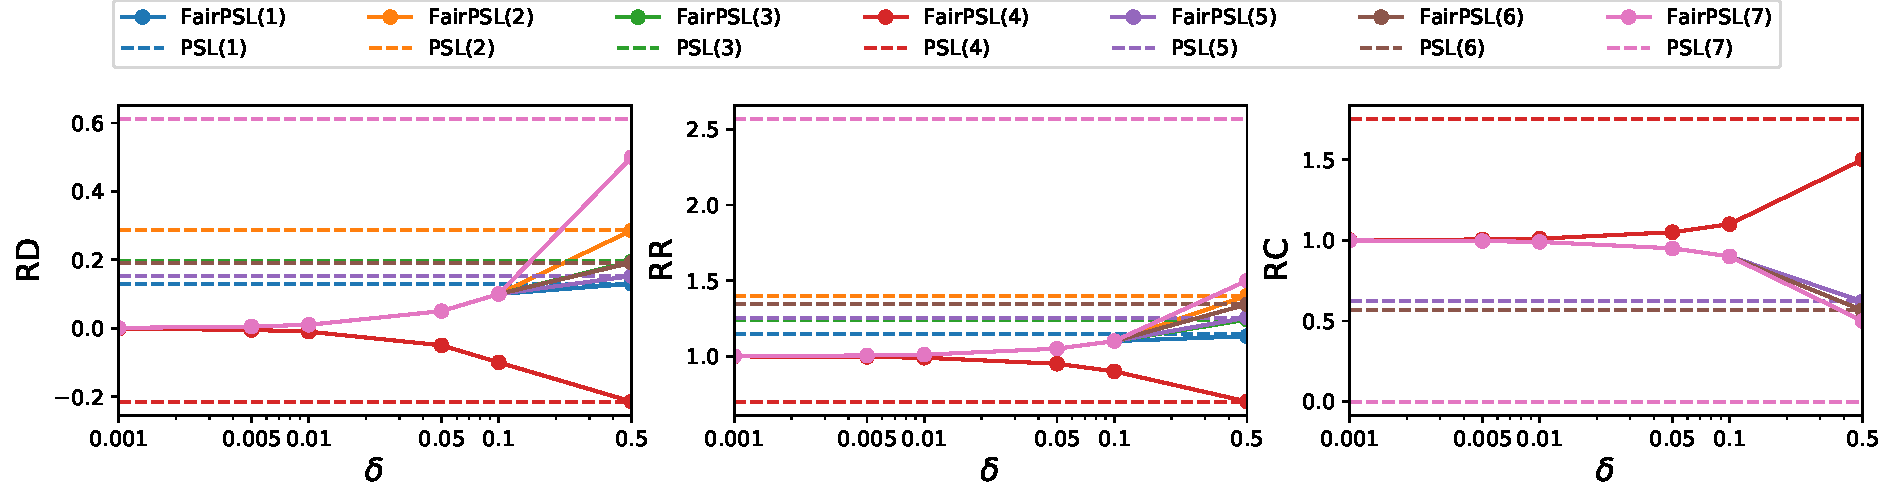
\includegraphics[width=1\linewidth]{figs/results_vis_uni_params.pdf}
\caption{\small Fairness score of predictions obtained by MAP inference of PSL and FairPSL, according to the fairness measures \emph{RD}, \emph{RR}, and \emph{RC}. The labels of datasets are mentioned with parenthesis next to the inference method. The FairPSL values of each measure are obtained by adding the $\delta$-fairness constraint of that measure.\label{fig:results}
}  
\end{figure}

To answer \textbf{Q1}, we run the MAP inference algorithm of PSL and FairPSL on seven synthetic datasets. 
We run the MAP inference of FairPSL multiple times on each dataset: For each of the three fairness measures, we add the corresponding $\delta$-fairness constraint with five thresholds $\{0.001, 0.005, 0.01, 0.05, 0.1, 0.5\}$.

Figure~\ref{fig:results} shows the fairness score of predictions in terms of the three fairness measures. As expected, tighter $\delta$-fairness constraints lead to better scores. Note that the best possible score according to RD is 0, as it computes a difference. Since RR and RC compute ratios, the best possible score according to these measures is 1. In our experiments, with any of these measures, taking $\delta = 0.001$ pushes the score of predictions to its limit.  

The $\delta$-fairness constraints modify the optimization problem of MAP inference by reducing the feasible region to solutions that conform with fairness guarantees. Research question \textbf{Q2} is concerned with the effect of this reduction on the accuracy of predictions. Note that decision quality is the same as the accuracy of predictions. To answer this question, we compare the inferred values for the decision atoms \textit{ToPromote(e)} against their actual values. These values are extracted from the known values of \textit{IsQualified(e)} according to rules 11 and 12 in Table~\ref{tab:pslmodel}. Figure~\ref{fig:accuracy} shows the area under the curve of the receiver operating characteristic~(AUC) of predicting the decision variable in three groups, namely the protected group, the unprotected group (i.e., promotion of the employees who have in-group managers), and all employees. By doing so, we make sure that our fairness constraints do not propagate bias towards either of the populations. Since the results of FairPSL with $\delta$-fairness constraints RR and RC are very similar to the results of RD, we only report the latter here.


\begin{figure}
    \centering
    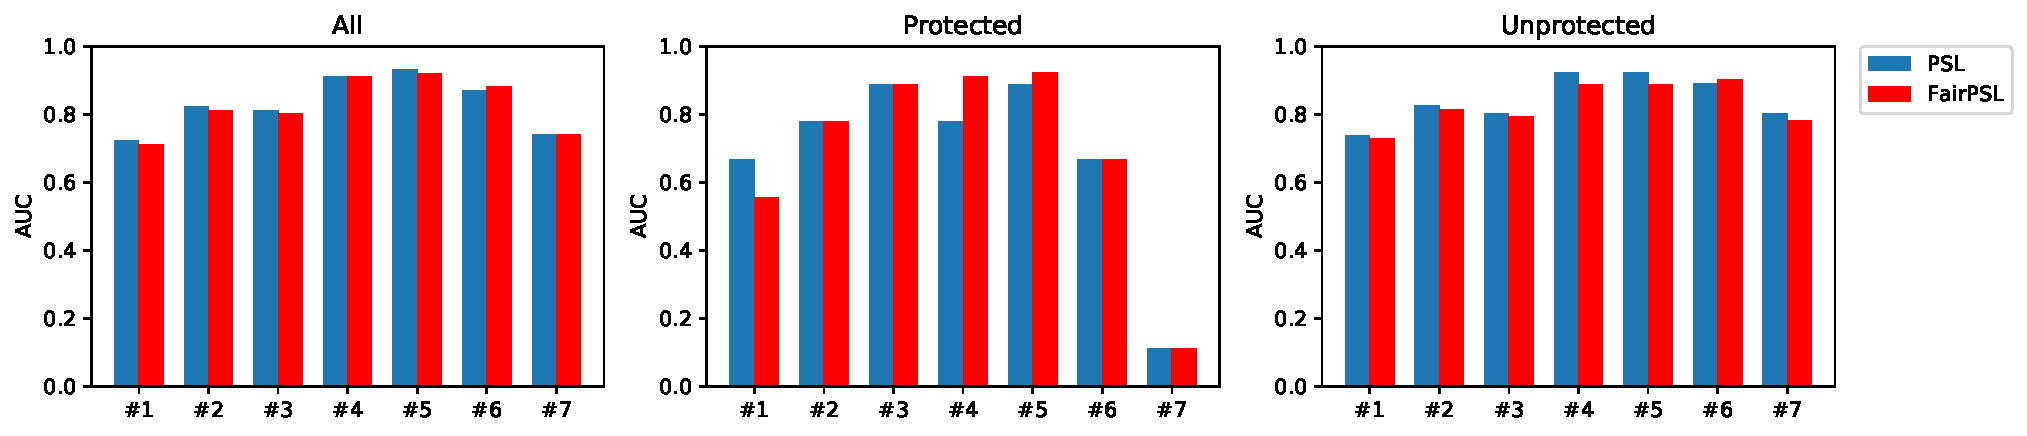
\includegraphics[width=\textwidth]{figs/roc.pdf}
    \caption{\small AUC score of predictions for truth values of unknown atoms \textit{ToPromote(e)} using MAP inference of PSL and FairPSL with $\delta$-fairness constraints $RD$ with $\delta=0.001$.}
    \label{fig:accuracy}
\end{figure}

According to Figure~\ref{fig:accuracy}, the results of both PSL and FairPSL in all seven datasets are close to each other. Note that although fairness may impose a cost in terms of overall accuracy, FairPSL often improves the accuracy of the protected class. Sometimes the overall predictions of FairPSL are even slightly better than PSL (e.g., dataset 6 and 7). As expected, the accuracy of the fourth setting where the opinions are unbiased are similar in both PSL and FairPSL. We observe that prediction of MAP inference for both FairPSL and PSL are similar, thus, in these settings at least, FairPSL guarantees fairness without hurting accuracy. Further investigation is required on the effect of the various ranges of discrimination (i.e., $\theta_1$, $\theta_2$, $\theta_3$, $\theta_4$) on the prediction results of FairPSL.



We also generate various types of organizations in which labels are not uniformly distributed, e.g., one population only occurs at the bottom levels of an organization. While we did not observe any differences in the behavior of our method with respect to accuracy and fairness measure, we found that the degree of discrimination is higher in such organizations. Further investigations on the structure of an organization on discrimination is an interesting direction for future research. 

\section{Conclusion and Future Directions}
\label{sec:conclusion}
Many applications of AI and machine learning affect peoples' lives in important ways. While there is a growing body of work on fairness in AI and ML, it assumes an individualistic notion of fairness.   In this paper, we have proposed a general framework for relational fairness which includes both a rich language for defining discrimination patterns and an efficient algorithm for performing inference subject to fairness constraints. We show our approach enforces fairness guarantees while preserving the accuracy of the predictions. 

There are many avenues for expanding on this work. For example, here we assumed that the discriminative pattern is given, however an automatic mechanism to extract discriminatory situations hidden in a large amount of decision records is an important and required task. Discrimination discovery has been studied for attribute-based fairness~\cite{pedreschi2013discovery}. An interesting next step is discrimination pattern discovery in relational data.

\section*{Acknowledgements}
This work is supported by the National Science Foundation under Grant Numbers CCF-1740850 and IIS-1703331. Golnoosh Farnadi and Behrouz Babaki are  supported by postdoctoral scholarships from IVADO through the Canada First Research Excellence Fund (CFREF) grant.

\begin{thebibliography}{10}
\itemsep=1pt 
\begin{small}

\bibitem{EUlaw}
European union legislation. (a) racial equality directive, 2000; (b) employment
  equality directive, 2000; (c) gender employment directive, 2006; (d) equal
  treatment directive (proposal), 2008.

\bibitem{UKlaw}
{UK} legislation. (a) sex discrimination act, 1975, (b) race relation act,
  1976.

\bibitem{USlaw}
United nations legislation. (a) universal declaration of human rights, 1948,
  (c) convention on the elimination of all forms of racial discrimination,
  1966, (d) convention on the elimination of all forms of discrimination
  against women, 1979.

\bibitem{alshukaili:iswc16}
Duhai Alshukaili, Alvaro A.~A. Fernandes, and Norman~W. Paton.
\newblock Structuring linked data search results using probabilistic soft
  logic.
\newblock In {\em International Semantic Web Conference {(1)}}, volume 9981 of
  {\em Lecture Notes in Computer Science}, pages 3--19, 2016.

\bibitem{bach:jmlr17}
Stephen~H. Bach, Matthias Broecheler, Bert Huang, and Lise Getoor.
\newblock Hinge-loss markov random fields and probabilistic soft logic.
\newblock {\em Journal of Machine Learning Research}, 18:109:1--109:67, 2017.

\bibitem{barocas2016big2}
Solon Barocas and Andrew~D Selbst.
\newblock Big data's disparate impact.
\newblock {\em California Law Review}, 104:671, 2016.

\bibitem{boyd2014networked}
Danah Boyd, Karen Levy, and Alice Marwick.
\newblock The networked nature of algorithmic discrimination.
\newblock In {\em Data and discrimination: Collected essays}, pages 53--57.
  2014.

\bibitem{brewer1979group}
Marilynn~B Brewer.
\newblock In-group bias in the minimal intergroup situation: A
  cognitive-motivational analysis.
\newblock {\em Psychological bulletin}, 86(2):307, 1979.

\bibitem{brewer2007social}
Marilynn~B Brewer.
\newblock The social psychology of intergroup relations: Social categorization,
  ingroup bias, and outgroup prejudice.
\newblock {\em Social Psychology: Handbook of Basic Principles}, 2007.

\bibitem{chouldechova2017fair2}
Alexandra Chouldechova.
\newblock Fair prediction with disparate impact: {A} study of bias in
  recidivism prediction instruments.
\newblock {\em CoRR}, abs/1703.00056, 2017.

\bibitem{dwork2012fairness3}
Cynthia Dwork, Moritz Hardt, Toniann Pitassi, Omer Reingold, and Richard~S.
  Zemel.
\newblock Fairness through awareness.
\newblock In {\em {ITCS}}, pages 214--226. {ACM}, 2012.

\bibitem{ebrahimi:emnlp16}
Javid Ebrahimi, Dejing Dou, and Daniel Lowd.
\newblock Weakly supervised tweet stance classification by relational
  bootstrapping.
\newblock In {\em {EMNLP}}, pages 1012--1017. The Association for Computational
  Linguistics, 2016.

\bibitem{farnadi2018fairness}
Golnoosh Farnadi, Behrouz Babaki, and Lise Getoor.
\newblock Fairness in relational domains.
\newblock In {\em AAAI/ACM Conference on AI, Ethics, and Society (AIES)}, pages
  108--114. ACM, 2018.

\bibitem{feldman2015certifying2}
Michael Feldman, Sorelle~A. Friedler, John Moeller, Carlos Scheidegger, and
  Suresh Venkatasubramanian.
\newblock Certifying and removing disparate impact.
\newblock In {\em {KDD}}, pages 259--268. {ACM}, 2015.

\bibitem{getoor2007introduction}
Lise Getoor and Ben Taskar.
\newblock {\em {Introduction to Statistical Relational Learning}}.
\newblock MIT press Cambridge, 2007.

\bibitem{hardt2016equality3}
Moritz Hardt, Eric Price, and Nati Srebro.
\newblock Equality of opportunity in supervised learning.
\newblock In {\em {NIPS}}, pages 3315--3323, 2016.

\bibitem{kamishima2011fairness}
Toshihiro Kamishima, Shotaro Akaho, and Jun Sakuma.
\newblock Fairness-aware learning through regularization approach.
\newblock In {\em ICDMW}, pages 643--650. {IEEE} Computer Society, 2011.

\bibitem{kouki:recsys15}
Pigi Kouki, Shobeir Fakhraei, James~R. Foulds, Magdalini Eirinaki, and Lise
  Getoor.
\newblock Hyper: {A} flexible and extensible probabilistic framework for hybrid
  recommender systems.
\newblock In {\em RecSys}, pages 99--106. {ACM}, 2015.

\bibitem{counterfactualfairness}
Matt~J. Kusner, Joshua~R. Loftus, Chris Russell, and Ricardo Silva.
\newblock Counterfactual fairness.
\newblock In {\em {NIPS}}, pages 4069--4079, 2017.

\bibitem{Pedreschi:2012}
Dino Pedreschi, Salvatore Ruggieri, and Franco Turini.
\newblock A study of top-k measures for discrimination discovery.
\newblock In {\em {SAC}}, pages 126--131. {ACM}, 2012.

\bibitem{pedreschi2013discovery}
Dino Pedreschi, Salvatore Ruggieri, and Franco Turini.
\newblock The discovery of discrimination.
\newblock In {\em Discrimination and Privacy in the Information Society},
  volume~3 of {\em Studies in Applied Philosophy, Epistemology and Rational
  Ethics}, pages 91--108. Springer, 2013.

\bibitem{ridgeway2004unpacking}
Cecilia~L Ridgeway and Shelley~J Correll.
\newblock Unpacking the gender system: A theoretical perspective on gender
  beliefs and social relations.
\newblock {\em Gender \& society}, 18(4):510--531, 2004.

\bibitem{sridhar:bioinformatics16}
Dhanya Sridhar, Shobeir Fakhraei, and Lise Getoor.
\newblock A probabilistic approach for collective similarity-based drug-drug
  interaction prediction.
\newblock {\em Bioinformatics}, 32(20):3175--3182, 2016.

\bibitem{verma2018fairness2}
Sahil Verma and Julia Rubin.
\newblock Fairness definitions explained.
\newblock In {\em 2018 IEEE/ACM International Workshop on Software Fairness
  (FairWare)}, pages 1--7. IEEE, 2018.

\bibitem{west2014exploiting}
Robert West, Hristo~S. Paskov, Jure Leskovec, and Christopher Potts.
\newblock Exploiting social network structure for person-to-person sentiment
  analysis.
\newblock {\em {TACL}}, 2:297--310, 2014.

\bibitem{zafar2017parity}
Muhammad~Bilal Zafar, Isabel Valera, Manuel Gomez{-}Rodriguez, Krishna~P.
  Gummadi, and Adrian Weller.
\newblock From parity to preference-based notions of fairness in
  classification.
\newblock In {\em {NIPS}}, pages 228--238, 2017.

\bibitem{zemel2013learning}
Richard~S. Zemel, Yu~Wu, Kevin Swersky, Toniann Pitassi, and Cynthia Dwork.
\newblock Learning fair representations.
\newblock In {\em {ICML} {(3)}}, volume~28 of {\em {JMLR} Workshop and
  Conference Proceedings}, pages 325--333. JMLR.org, 2013.

\end{small}
\end{thebibliography}

\end{document}

\end{article}

\begin{article}
{XuanYuan: An AI-Native Database}
{Guoliang Li, Xuanhe Zhou, Sihao Li}
\graphicspath{{submissions/ainative/}}
%\documentclass[11pt,dvipdfm]{article}
\documentclass[11pt]{article}
\usepackage{deauthor,times,graphicx} %required
\usepackage{amsmath,amssymb}
\usepackage{multirow}
\usepackage{algorithm}
\usepackage{algpseudocode}
\usepackage{todonotes}
\usepackage{url}

% \graphicspath{{farnadi/}}

\newtheorem{mydef}{\textbf{Definition}}
\newtheorem{myex}{\textbf{Example}}
\newtheorem{mytheorem}{\textbf{Theorem}}


\begin{document}

\title{A Declarative Approach to Fairness in Relational Domains}
\author{Golnoosh Farnadi$^{1,2}$, Behrouz Babaki$^1$, Lise Getoor$^3$\\
$^1$Polytechnique Montr\'{e}al, $^2$ Mila, $^3$ UC Santa Cruz \\
farnadig@mila.quebec, behrouz.babaki@polymtl.ca, getoor@soe.ucsc.edu}

\maketitle

\begin{abstract}
AI and machine learning tools are being used with increasing frequency for decision making in domains that affect peoples' lives such as employment, education, policing and %loan approval
financial qualifications. These uses raise concerns about biases of algorithmic discrimination and have motivated the development of fairness-aware machine learning. However, existing fairness approaches are based solely on attributes of individuals. In many cases, discrimination is much more complex, and taking into account the social, organizational, and other connections between individuals is important. We introduce new notions of fairness that are able to capture the relational structure in a domain. We use first-order logic to provide a flexible and expressive language for specifying complex relational patterns of discrimination. Furthermore, we extend an existing statistical relational learning framework, probabilistic soft logic~(PSL), to incorporate our definition of relational fairness. We refer to this fairness-aware framework FairPSL. FairPSL makes use of the logical definitions of fairnesss but also supports a probabilistic interpretation. In particular, we show how to perform maximum a posteriori~(MAP) inference by exploiting probabilistic dependencies within the domain while avoiding violations of fairness guarantees. Preliminary empirical evaluation shows that we are able to make both accurate and fair decisions.
\end{abstract}

\section{Introduction}
\label{sec:introduction}

Over the past few years, AI and machine learning have become essential components in operations that drive the modern society, e.g., in financial, administrative, and educational spheres. \emph{Discrimination} happens when qualities of individuals which are not relevant to the decision making process influence the decision. Delegating decision making to an automated process raises questions about discriminating against individuals with certain traits based on biases in the data. This is especially important when the decisions have the potential to impact the lives of individuals, for example, the decisions on granting loans, assigning credit, and employment. 

\emph{Fairness} is defined as the absence of discrimination in a decision making process. The goal of \emph{fairness-aware} machine learning is to ensure that the decisions made by an algorithm do not discriminate against a population of individuals~\cite{feldman2015certifying2,boyd2014networked,hardt2016equality3}. Fairness has been well studied in the social sciences and legal scholarship (for an in-depth review see~\cite{barocas2016big2}), and there is emerging work on fairness-aware ML within the AI and computer science communities. For example, fairness through awareness/Lipschitz property~\cite{dwork2012fairness3}, individual fairness~\cite{zemel2013learning}, statistical parity/group fairness~\cite{kamishima2011fairness}, counterfactual fairness~\cite{counterfactualfairness}, demographic parity/disparate impact~\cite{feldman2015certifying2,chouldechova2017fair2}, preference-based fairness~\cite{zafar2017parity}, and equality of opportunity~\cite{hardt2016equality3}.

The existing work in fairness-aware machine learning is based on a definition of discrimination where a decision is influenced by an \emph{attribute} of an individual. An attribute value upon which discrimination is based (such as gender, race, or religion) is called a \emph{sensitive attribute}. The sensitive attribute defines a population of vulnerable individuals known as the \emph{protected group}. A fair decision-making process treats the protected group the same as the \emph{unprotected group}. 

However, in many social contexts, discrimination is the result of complex interactions and can not be described solely in terms of attributes of an individual. For example, consider an imaginary scenario in an organization in which younger female workers who have older male supervisors have lower chances of promotion than their male counterparts.\footnote{Of course, many other patterns may be possible: female bosses may promote female subordinates and discriminate against male workers, or male bosses may promote female employees.  Our goal is to provide a general framework which is able to describe arbitrarily complex discrimination patterns.} 
 This discrimination pattern involves two attributes of the individual (gender and age), a relationship with another individual (supervisor), and two attributes of the second individual. Addressing such complex cases poses two challenges. First, the concepts of discrimination and fairness need to be extended to capture not only attributes of individuals but also the relationships between them. Second, a process is required that ensures that fair decisions are made about individuals who are affected by such patterns. In this paper we address both of these challenges.
We use first-order logic (FOL) to extend the notion of fairness to the relational setting. FOL is an expressive representation for relational problems which is also widely used for learning in relational domains. Moreover, we extend an existing framework for statistical relational learning~\cite{getoor2007introduction} called probabilistic soft logic (PSL)\footnote{http://psl.linqs.org/}~\cite{bach:jmlr17}. PSL combines logic and probability for learning and reasoning over uncertain relational domains. One of the most common reasoning tasks in PSL is called maximum a posteriori (MAP) inference, which is performed by finding the most probable truth values for unknowns over a set of given evidence. We develop a new MAP inference algorithm which is able to maximize the a posteriori values of unknown variables \emph{subject to} fairness guarantees. An early version of this paper which this work builds upon and extends appeared in~\cite{farnadi2018fairness}.

\looseness-1
Our contributions are as follows: 1) we propose fairness-aware machine learning for the relational setting; 2) we extend PSL into a fairness-aware framework called FairPSL which can represent the logical definition of fairness; 3) we develop a new MAP inference algorithm which is able to maximize the posteriori values of unknown variables \emph{subject to} fairness guarantees; 4) we empirically evaluate our proposed framework on synthetic data. 

\section{Motivation}
\label{sec:motivation}

Discrimination in social contexts have been studied in the field of social psychology~\cite{brewer2007social,brewer1979group,ridgeway2004unpacking}. There is a large literature on various aspects of relational bias in social contexts such as \emph{in-group-out-group bias}, \emph{gender bias}, and \emph{ethnicity-based favoritism} that can result in discrimination. 
As an example, consider gender bias in the workplace that reflects stereotypically masculine criteria and male-based favoritism. Such gender bias 
typically places women in lower positions and negatively impacts their opportunities. Further, lack of women in leadership positions may affect the promotion of women and results in a glass ceiling that keeps women from rising beyond a certain level in the hierarchy. This scenario shows that considering  protected attributes such as gender is not always sufficient to detect the source of bias and avoid discrimination, one also has to consider the relational information, in this case the organization hierarchy. Note that this can be generalized to any ingroup/outgroup scenario where the sensitive attribute could be race, religion, age, marital-status, etc.

The existing work on designing fair algorithms in machine learning exclusively focuses on \emph{attribute-based fairness}, which is based on the following assumptions: First, there is an assumption that the individuals (sometimes referred to as units or entities) are independent and described by simple attribute vectors. Second, the group for which one wishes to ensure fairness (known as the \emph{protected group}) is defined on the basis of some attribute values. Finally, there is a decision that is associated with each individual, and the goal is to ensure that members of the protected group are subject to a fair decision (we discuss different fairness measures in Section~\ref{sec:fairnessmeasure}).  We illustrate  attribute-based fairness in the following example. 

\begin{myex}[Loan Processing]
\label{ex:loan}
A bank bases its decisions about granting a loan on attributes of the applicant. The goal is to decide whether to grant a loan to an applicant using a predictive model. The bank needs to ensure that the obey fair lending practices and ensure that gender, race, sexual orientation of applicants has no influence on the decision. In this scenario, the protected group is the historically disadvantaged applicants.  
\end{myex}
The current fairness-aware machine learning techniques are not capable of modeling relations and hence cannot be used to make the decision making model fair. However, in many decision making scenarios, especially in social and organizational settings, the domain is relational, and the protected group itself might be best represented using a relational definition. We illustrate this setting in the following scenario:
\begin{myex}[Performance Review]
\label{ex:review}
Consider an organization where decisions about the promotion of employees is based on two criteria: 1) an objective performance measure, and 2) the opinion of their direct and indirect managers above them. The opinions are inferred from the performance reviews which are collected periodically. Not every manager can submit a review for all its subordinates, this is especially the case for top-level managers who have a large number of subordinates. Hence, the opinions of managers are collectively inferred from the opinions of their sub-ordinates. However, some employees may be biased, and judge other employees unfavorably, by favoring employees who are similar to themselves (same gender, race, religion, etc.) over employees who are dissimilar. The organization needs to ensure that promotion of employees do not have any relational bias caused by in-group-out-group favoritism.

\end{myex}
Example~\ref{ex:review} describes a prediction problem over a database that consists of relations between employees. Such prediction tasks are best handled by techniques from the relational learning domain. To ensure fair prediction in such settings, we need to extend the notion of \emph{attribute-based fairness} to \emph{relational fairness}. Throughout this paper, we use the performance review problem as a running example for relational fairness.

\section{Fairness Formalism}
\label{sec:formulation}

A representation that can describe different types of entities and different relationships between them is called relational. In this section, we use first-order logic to define relational fairness. We employ first-order logic as an expressive representation formalism which can represent objects and complex relationships between them. We start by defining an atom:

\begin{mydef}[Atom]
An atom is an expression of the form $P(a_1, a_2, \ldots, a_n)$ where each argument $a_1, a_2,$ $\ldots,$ $a_n$ is either a constant or a variable. The finite set of all possible substitutions of a variable to a constant for a particular variable $a$ is called its \textit{domain} $D_{a}$. If all variables in $P(a_1, a_2, \ldots, a_n)$ are substituted by some constant from their respective domain, then we call the resulting atom a \textit{ground atom}. 
\end{mydef}

\begin{myex}
In our loan processing problem (Example~\ref{ex:loan}), we can represent applicants' attributes by atoms. For instance, atom $Female(v)$ indicates whether or not applicant $v$ is female. Similarly, we can represent relations with atoms. In the performance review problem in Example~\ref{ex:review} the atom $Manager(m,e)$ indicates whether or not employee $m$ is a direct or indirect manager of employee $e$.
\end{myex}

The relational setting provides the flexibility to express complex definitions with formulae.

\begin{mydef}[Formula] 
A formula is defined by induction: every atom is a formula. If $\alpha$ and $\beta$ are formulae, then $\alpha \vee \beta$, $\alpha \wedge \beta$, $\neg \alpha$, $\alpha \rightarrow \beta$ are formulae. If $x$ is a variable and $\alpha$ is a formula, then the quantified expressions of the form $\exists x$ $\alpha$ and $\forall x$ $\alpha$ are formulae.    
\end{mydef}

To characterize groups of individuals based on a formula, we define the notion of \emph{population}.

\begin{mydef}[Population]
We denote formula $F$ which has only one free variable $v$ (i.e., other variables in $F$ are quantified) by $F[v]$. The population defined by $F[v]$ is the set of substitutions of $v$ for which $F[v]$ holds.   
\end{mydef}


\begin{myex}
\label{ex:disformula}
Consider the formula $F[v] := \forall u, \, \textit{Manager}(u,v) \rightarrow \neg \textit{SameGroup}(u, v)$. The population specified by this formula is the set of individuals all of whose managers belong to a group different from theirs. 
\end{myex}

The truth value of a formula is derived from the truth value of atoms that it comprises, according to the rules of logic. Each possible assignment of truth values to ground atoms is called an \emph{interpretation}. 


\begin{mydef}[Interpretation]
An interpretation $I$ is a mapping that associates a truth value $I(P)$ to each ground atom $P$. For Boolean truth values, $I$ associates true to 1 and false to 0 truth values. For soft logic (see Definition~\ref{def:softlogic}) $I$ maps each ground atom $P$ to a truth value in interval $[0, 1]$.
\end{mydef}

In attribute-based fairness, it is assumed that there is a certain attribute of individuals, i.e, the sensitive attribute,  that we do not want to affect a decision. Gender, race, religion and marital status are examples of sensitive attributes. Discrimination has been defined in social science studies as a treatment in favor or against a group of individuals given their sensitive attribute. This group of individuals is the protected group. 

In a relational setting, both the sensitive attributes of an individual and their participation in various relations may have an undesired effect on the final decision. We characterize the protected group in a relational setting by means of a population. In practice, we are often interested in maintaining fairness for a specific population such as applicants, students, employees, etc. This population is then partitioned into the protected and unprotected groups. We define a \emph{discriminative pattern} which is a pair of formulae to capture these groups: 1) $F_1[v]$: to specify the difference between the protected and unprotected groups and 2) $F_2[v]$: to specify the population over which we want to maintain fairness. 

\begin{mydef}[Discriminative pattern]
A discriminative pattern is a pair $\textit{DP}[v]:=(F_1[v], F_2[v])$ , where $F_1[v]$ and $F_2[v]$ are formulae.
\end{mydef}

\begin{myex}
\label{ex:pattern}
The two formulae in the discrimination pattern $\textit{DP}[v]:= \big((\forall u, \,  \textit{Manager}(u,v) \rightarrow  \neg \textit{SameGroup}(u, v)),$ $\textit{Employee}(v)\big)$ specify two populations, namely all employees and those employees who belong to a group different from their managers.
\end{myex}

Given the definition of the discriminative pattern, we have a rich language to define the scope of the protected and unprotected groups in a relational setting.

\begin{mydef}[Protected group] Given an interpretation $I$, the protected group is a population of the form:
{$$PG :=\{ v : F_1[v] \wedge F_2[v]\}$$}
which is defined as the set of all instances hold for variable $v$ for which $F_1[v] \wedge F_2[v]$ is true under interpretation $I$, that is, $I(F_1[v] \wedge F_2[v]) = 1$. 
Similarly, the \emph{unprotected group} is a population of the form: 
{$$UG := \{ v : \neg F_1[v] \wedge  F_2[v]\}$$}
which is defined as the set of all instances hold for variable $v$ 
for which $I(\neg F_1[v] \wedge F_2[v]) = 1$. 
\end{mydef}

\begin{myex}
The protected group of the discrimination pattern specified in Example~\ref{ex:pattern} is {$PG := \big\{ v : \big(\forall u, \,$ $ \textit{Manager}(u, v) \rightarrow \neg \textit{SameGroup}(u, v)\big) \wedge \textit{Employee}(v) \big\}$} and the unprotected group is {$UG :=  \big\{ v:  \big(\exists u, \, \textit{Manager}(u,v) \wedge \textit{SameGroup}(u, v)\big) \wedge \textit{Employee}(v) \big\}$}. This means our protected group is the set of employees belonging to a group different from their managers,
and our unprotected group consists of other employees. 
\end{myex}

Discrimination is defined in terms of a treatment or decision that distinguishes between the protected and unprotected groups. Here we define the \emph{decision} atom.
\begin{mydef}[Decision atom] A decision atom $d(v)$ is an atom containing exactly one variable $v$ that specifies a decision affecting the protected group which is defined either by law or end-user.
\end{mydef}
\begin{myex}
The decision atom ${\textit ToPromote}(v)$ indicates whether or not $v$ receives a promotion.
\end{myex}

Note that the fairness formulation in this section is designed for the relational setting, however relational fairness subsumes the attribute-based fairness such that: a sensitive attribute is defined by an atom with one argument and $F_2[v]$ in discrimination pattern is $\textit{Applicant}(v)$. For example, discrimination pattern of our loan processing problem in Example~\ref{ex:loan} is of the form $\textit{DP} := ( \textit{Female}(v), \textit{Applicant}(v))$ that denotes female applicants as the protected group (i.e., $PG :=  \{ v: \textit{Female}(v) \}$) and male applicants as the unprotected group (i.e., $UG := \{ v: \neg \textit{Female}(v)\}$).


\section{Fairness Measures}
\label{sec:fairnessmeasure}

Over the past few years, many fairness measures have been introduced~\cite{verma2018fairness2}. An important class of these measures are \emph{group fairness} measures which quantify the inequality between different subgroups. Some of the most popular measures in this class include \emph{equal opportunity}, \emph{equalized odds}, and \emph{demographic parity}~\cite{hardt2016equality3}. In this paper we restrict our focus to the latter. In an attribute-value setting, demographic parity means that the decision should be independent of the protected attributes. Assume that binary variables $A$ and $C$ denote the decision and protected attributes, and the preferred value of $A$ is one. Demographic parity requires that:

\begin{equation*}
    P(A=1 | C=0) = P(A=1 | C=1)
\end{equation*}

We will now generalize this measure to the relational setting using the notations defined in Section~\ref{sec:formulation}. Let $a$ and $c$ denote the counts of denial (i.e., negative decisions) for protected and unprotected groups, and $n_{1}$ and $n_{2}$ denote their sizes, respectively. Given the decision atom $d(v)$, discriminative pattern $\textit{DP}(F_1[v], F_2[v])$, and interpretation $I$, these counts are computed by the following equations: 
{
\begin{flalign}
    & a \equiv \sum_{v \in D_v} I\big( \neg d(v) \wedge  F_1[v] \wedge F_2[v]) \label{eq:a}\\
    & c \equiv \sum_{v \in D_v} I\big( \neg d(v) \wedge  \neg F_1[v] \wedge  F_2[v]) \label{eq:c}\\
    & n_{1} \equiv \sum_{v \in D_v} I\big(F_1[v] \wedge F_2[v]) \label{eq:n1}\\
    & n_{2} \equiv \sum_{v \in D_v} I\big(\neg F_1[v] \wedge  F_2[v]) \label{eq:n2}
\end{flalign}}
The proportions of denying for protected and unprotected groups are $p_1 = \frac{a}{n_1}$ and $p_2 = \frac{c}{n_2}$, respectively. There are a number of data-driven measures~\cite{Pedreschi:2012} which quantify demographic disparity and can be defined in terms of $p_1$ and $p_2$:
\begin{itemize}
    \item \textbf{Risk difference}: $RD = p_1 - p_2$, also known as absolute risk reduction. 
    \item \textbf{Risk Ratio}: $RR = \frac{p_1}{p_2}$, also known as relative risk. 
    \item \textbf{Relative Chance}: $RC = \frac{1 - p_1}{1 - p_2}$ also, known as selection rate.
\end{itemize}
These measures have been used in the legal systems of European Union, UK, and US~\cite{EUlaw,UKlaw,USlaw}. Notice that RR is the ratio of the proportion of benefit denial between the protected and unprotected groups, while RC is the ratio of the proportion of benefit granted. Finally, we introduce the notion of $\delta$-fairness.

\begin{mydef}[$\delta$-fairness]
If a fairness measure for a decision making process falls within some $\delta$-window, then the process is \emph{$\delta\text{-fair}$}. Given $0 \leq \delta \leq 1$, the  $\delta$-windows for measures RD/RR/RC are defined as:
{\begin{flalign*}
	     - \delta \leq &RD \leq \delta \\
	     1- \delta \leq &RR \leq 1+ \delta\\
	     1- \delta \leq &RC \leq 1+ \delta
	\end{flalign*}}
\end{mydef}

To overcome the limitations of attribute-based fairness, we introduce a new statistical relational learning~(SRL) framework~\cite{getoor2007introduction} suitable for modelling fairness in relational domain. In the next section, we review probabilistic soft logic~(PSL). We then extend PSL with the definition of relational fairness introduced above in Section~\ref{sec:fairMAP}. Our fairness-aware framework, ``FairPSL'', is the first SRL framework that performs fair inference. 

\section{Background: Probabilistic Soft Logic}
\label{sec:psl}

In this section, we review the syntax and semantics of PSL, and in the next section we extend MAP inference in PSL with fairness constraints to define MAP inference in FairPSL.

PSL is a probabilistic programming language for defining hinge-loss Markov random fields~\cite{bach:jmlr17}. Unlike other SRL frameworks whose atoms are Boolean, atoms in PSL can take continuous values in the interval $[0,1]$. PSL is an expressive modeling language that can incorporate domain knowledge with first-order logical rules and has been used successfully in various domains, including bioinformatics~\cite{sridhar:bioinformatics16}, recommender systems~\cite{kouki:recsys15}, natural language processing~\cite{ebrahimi:emnlp16}, information retrieval~\cite{alshukaili:iswc16}, and social network analysis~\cite{west2014exploiting}, among many others. 
 
A PSL model is defined by a set of first-order logical rules called \emph{PSL rules}.

\begin{mydef} [PSL rule] a PSL rule $r$ is an expression of the form:
{\begin{equation}
\lambda_{r}: T_1 \land T_2 \land \ldots \land T_w \rightarrow H_1 \vee H_2 \vee \ldots \vee H_l
\end{equation}}

where { $T_1, T_2, \ldots, T_w, H_1, H_2, \ldots, H_l$} are atoms or negated atoms and { $\lambda_{r} \in \mathbb{R}^{+} \cup \infty$} is the weight of the rule $r$.  We call { $T_1 \land T_2 \land \ldots \land T_w$} the body of $r$ ($r_{body}$), and { $H_1 \vee H_2 \vee \ldots \vee H_l$} the head of $r$ ($r_{head}$).
\end{mydef}


Since atoms in PSL take on continuous values in the unit interval $[0,1]$, next we define soft logic to calculate the value of the PSL rules under an interpretation $I$.

\begin{mydef}[Soft logic]
\label{def:softlogic}
The ({$\tilde{\wedge}$}) and ({$\tilde{\vee}$}) and negation ({$\tilde{\neg}$}) are defined as follows. For {$m, n \in [0,1]$} we have: {$m \tilde{\wedge} n = \max(m+n -1, 0)$}, {$m \tilde{\vee} n = \min(m+n , 1)$} and {$\tilde{\neg} m = 1 - m$}. The $\, \tilde{} \,$ indicates the relaxation over Boolean values.
\end{mydef}

The probability of truth value assignments in PSL is determined by the rules' \emph{distance to satisfaction}.

\begin{mydef}[The distance to satisfaction]
The distance to satisfaction $d_{r}(I)$ of a rule $r$ under an interpretation $I$ is defined as:
{
\begin{equation}
d_{r}(I) = \max\{0, I(r_{body})-I(r_{head})\}
\end{equation}}
\end{mydef}

By using Definition~\ref{def:softlogic}, one can show that the closer the interpretation of a grounded rule $r$ is to 1, the smaller its distance to satisfaction. A PSL model induces a distribution over interpretations $I$. Let $R$ be the set of all grounded rules, then the probability density function is:
{
\begin{equation}
f(I) ={\frac{1}{Z}} \exp[-\sum_{r\in R} \lambda_{r}(d_{r}(I))^p]
\label{eq:potential}
\end{equation}
}
\noindent where { $\lambda_{r}$} is the weight of rule $r$, {
$Z = \int_{I} \exp[ -\sum_{r\in R} \lambda_{r}(d_{r}(I))^p]$
} is a normalization constant, and { $p \in \{1,2\}$} provides a choice of two different loss functions, $p=1$ (i.e., linear), and $p=2$ (i.e, quadratic). These probabilistic models are instances of hinge-loss Markov random fields~(HL-MRF)~\cite{bach:jmlr17}. The goal of maximum a posteriori (MAP) inference is to find the most probable truth assignments $I_{\textit{MPE}}$ of unknown ground atoms given the evidence which is defined by the interpretation $I$. Let $X$ be all the evidence, i.e., $X$ is the set of ground atoms such that $\forall x \in X, I(x)$ is known, and let $Y$ be the set of ground atoms such that $\forall y \in Y, I(y)$ is unknown. Then we have
{
\begin{equation}
I_{\textit{MAP}}(Y) = \textit{arg}\max_{I(Y)} P(I(Y)|I(X))
\end{equation}}
Maximizing the density function in Equation~\ref{eq:potential} is equivalent to minimizing the weighted sum of the distances to satisfaction of all rules in PSL. 

\begin{table*}[t]
    \centering
    \begin{tabular}{|lll|}
    \hline
    &&\\
    $R1$ & $\lambda_1$ &: $\textit{IsQualified}(e) \rightarrow \textit{HighPerformance}(e)$ \\
    $R2$ & $\lambda_1$ &: $\neg \textit{IsQualified}(e) \rightarrow \neg \textit{HighPerformance}(e)$ \\
    $R3$ & $\infty$ &: $\textit{PositiveReview}(e1, e2) \rightarrow \textit{PositiveOpinion}(e1, e2)$ \\
    $R4$ & $\infty$ &: $\neg \textit{PositiveReview}(e1, e2) \rightarrow \neg \textit{PositiveOpinion}(e1, e2)$ \\
    $R5$ & $\lambda_1$ &: $\textit{PositiveOpinion}(e1, e2) \wedge \textit{Manager}(m, e1) \rightarrow \textit{PositiveOpinion}(m, e2)$ \\
    $R6$ & $\lambda_1$ &: $\neg \textit{PositiveOpinion}(e1, e2) \wedge \textit{Manager}(m, e1) \rightarrow \neg \textit{PositiveOpinion}(m, e2)$ \\
    $R7$ & $\lambda_1$ &: $\textit{PositiveOpinion}(m, e) \wedge \textit{Manager}(m, e) \rightarrow \textit{IsQualified}(e)$ \\
    $R8$ & $\lambda_1$ &: $\neg \textit{PositiveOpinion}(m, e) \wedge \textit{Manager}(m, e) \rightarrow \neg \textit{IsQualified}(e)$ \\
    $R9$ &  $\lambda_1$ &: $\neg \textit{ToPromote}(e)$\\
    $R10$ & $\infty$ &: $\textit{IsQualified}(e) \rightarrow \textit{ToPromote}(e)$ \\
    $R11$ & $\infty$ &: $\neg \textit{IsQualified}(e) \rightarrow \neg \textit{ToPromote}(e)$ \\
    &&\\
    \hline
    \end{tabular}
    \caption{\small A simplified PSL model for the \emph{Performance Reviewing} problem}
    \label{tab:pslmodel}
\end{table*}

\begin{myex}
\label{ex:pslmodel}
The simplified PSL model for the performance reviewing problem in Example\ref{ex:review} is given in Table~\ref{tab:pslmodel}. The goal of MAP inference for this problem is to infer employees to promote. We simplified the model by assigning the same weight to all soft rules (i.e., $\lambda_i= 1$ where $i=\{1,2,5,6,7,8,9\}$). Below we explain the meaning of each rule in the model.

Rule $R1$ indicates that qualified employees have high performance and similarly rule $R2$ expresses that a negative qualification of employees is derived from their low performance. Rules $R5$ and $R6$ presents the propagation of opinion from bottom to top of the organizational hierarchy, i.e., managers have similar opinions towards employees given the opinions of their sub-ordinate managers. And rules $R7$ and $R8$ indicate that the positive/negative opinion of direct/indirect managers derive from the qualification of an employee. Rule $R9$ indicates the prior that not all employees get promoted. We also have four hard constraints (i.e., rules $R3$, $R4$, $R10$ and $R11$) where the weight of the rules are $\infty$. Rules $R3$ and $R4$ indicate that submitted positive/negative reviews should reflect positive/negative opinions. And two rules $R10$ and $R11$ show that a highly qualified employee should get promoted. 
\end{myex}

\section{Fairness-aware PSL (FairPSL)}
\label{sec:fairMAP}

The standard MAP inference in PSL aims at finding values that maximize the conditional probability of unknowns. Once a decision is made according to these values, one can use the fairness measure to quantify the degree of discrimination. A simple way to incorporate fairness in MAP inference is to add the $\delta$-fairness constraints to the corresponding optimization problem.   

Consider risk difference, $\textit{RD}$, where $\textit{RD} \equiv \frac{\mathbf{a}}{n_1} - \frac{\mathbf{c}}{n_2}$. The $\delta$-fairness constraint $-\delta \leq \textit{RD} \leq \delta$ can be encoded as the following constraints:
{\begin{align}
    & n_2 \mathbf{a} - n_1 \mathbf{c} - n_1 n_2 \delta \leq 0 \label{eq:RD1}\\
    & n_2 \mathbf{a} - n_1 \mathbf{c} + n_1 n_2 \delta \geq 0
\end{align}}
Similarly, from $\textit{RR} \equiv \frac{\mathbf{a} / n_1}{\mathbf{c} / n_2}$ and the $\delta$-fairness constraint $1 - \delta \leq \textit{RR} \leq 1 + \delta$ we obtain:
{\begin{align}
    & n_2 \mathbf{a} - (1 + \delta) n_1 \mathbf{c} \leq 0 \\
    & n_2 \mathbf{a} - (1 - \delta) n_1 \mathbf{c} \geq 0
\end{align}}
And finally, $\textit{RC} \equiv \frac{1 - \mathbf{a} / n_1}{1 - \mathbf{c} / n_2}$ and the $\delta$-fairness constraint $1 - \delta \leq \textit{RC} \leq 1 + \delta$ gives:
{ \begin{align}
    & - n_2 \mathbf{a} + (1 + \delta) n_1 \mathbf{c} - \delta n_1 n_2 \leq 0 \\
    & - n_2 \mathbf{a} + (1 - \delta) n_1 \mathbf{c} + \delta n_1 n_2 \geq 0 \label{eq:RC2}
\end{align}}
A primary advantage of PSL over similar frameworks is that its MAP inference task reduces to a convex optimization problem which can be solved in polynomial time. To preserve this advantage, we need to ensure that the problem will remain convex after the addition of $\delta$-fairness constraints. 

\begin{mytheorem}
The following condition is sufficient for preserving the convexity of MAP inference problem after addition of $\delta$-fairness constraints: The formulae $F_1[v]$ and $F_2[v]$ do not contain an atom $y \in Y$ and all atoms in $F_1[v]$ and $F_2[v]$ have values zero or one.
\end{mytheorem}
\begin{proof}
Since $I(F_1[v])$ and $I(F_2[v])$ do not depend on $I(Y)$, the values $n_{1}$ and $n_{2}$ are constants that can be computed in advance. Let us define the sets $D_v^a = \{ v \in D_v : F_1[v] \wedge F_2[v] \, \text{is true} \}$ and $D_v^c = \{ v \in D_v : \neg F_1[v] \wedge F_2[v] \, \text{is true} \}$. Since $F_1[v]$ and $F_2[v]$ can be only zero or one, we can rewrite the equations~\ref{eq:a} and \ref{eq:c} as:
{
\begin{align*}
    & \mathbf{a} = \sum_{v \in D_v^a} I(\neg d(v)) = |D_v^a| - \sum_{v \in D_v^a} I(d(v))\\
    & \mathbf{c} = \sum_{v \in D_v^c} I(\neg d(v)) = |D_v^c| - \sum_{v \in D_v^c} I(d(v))
\end{align*}}
\noindent which indicates that $\mathbf{a}$ and $\mathbf{c}$ can be expressed as linear combinations of variables in the optimization problem. This means that constraints~\ref{eq:RD1}-\ref{eq:RC2} are linear. Hence, addition of these constraints preserves the convexity of the optimization problem. 
\end{proof}

\section{Experiments}
\label{sec:experiment}

\begin{figure}
  \begin{minipage}[c]{0.6\textwidth}
    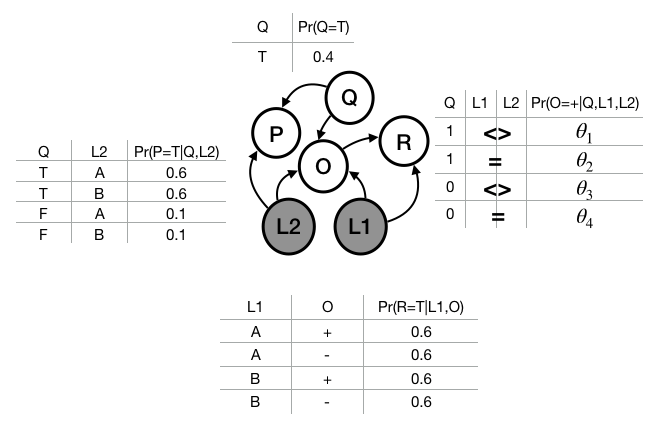
\includegraphics[width=\textwidth]{figs/BN.png}
  \end{minipage}\hfill
  \begin{minipage}[c]{0.45\textwidth}
    \caption{
        \small The model used for generating the datasets. There are four binary random variables, P, Q, O, and R. \textbf{P}: indicates whether or not the employee has high performance; \textbf{Q}: indicates whether or not an employee has high qualification; \textbf{O}: indicates whether or not the colleague submits the positive opinion towards the employee;  \textbf{R}: indicates whether or not the colleague has a positive opinion towards the employee;  \textbf{L1, L2}: indicates the label of the review provider and review receiver (observed).
    } \label{fig:BN}
  \end{minipage}
\end{figure}

We show the effectiveness of FairPSL by performing an empirical evaluation. We investigate two research questions in our experiments:
\begin{description}
\item[Q1] What is the effect of the fairness threshold $\delta$ on the fairness measures $RD/RC/RR$?
\item[Q2] How is decision quality affected by imposing $\delta$-fairness constraints?
\end{description}

Note that although we present the result for specific parameters of the framework in this section, we ran extensive analysis and the results we present are representative. We implemented the MAP inference routines of PSL and FairPSL in Python, using Gurobi-8.1\footnote{\url{www.gurobi.com}} as the backend solver. The FairPSL code, code for the data generator and data is publicly available\footnote{https://github.com/gfarnadi/FairPSL}. 

\subsection{Data generation}
  
We evaluate the FairPSL inference algorithm on synthetic datasets representing the performance review scenario (introduced in Example~\ref{ex:review}). The organization hierarchy is generated synthetically. 
The organization hierarchy generator is parameterized by two numbers: the number of employees in the organization ($n$) and the number of employees managed by each manager ($k$). Each employee is randomly assigned with a label \emph{A} or \emph{B}. An examples organization hierarchy with $n$=50 and $k$=3 is shown in Figure~\ref{fig:hierachy}.

\begin{figure}
  \begin{minipage}[c]{0.3\textwidth}
    \caption{
        \small An example of an organizational hierarchy with five levels and 50 employees with k=3. Each employee either has label A (shown with grey) or B (shown with white).
    }\label{fig:hierachy} 
	\end{minipage} \hfill
    \begin{minipage}[c]{0.7\textwidth}
    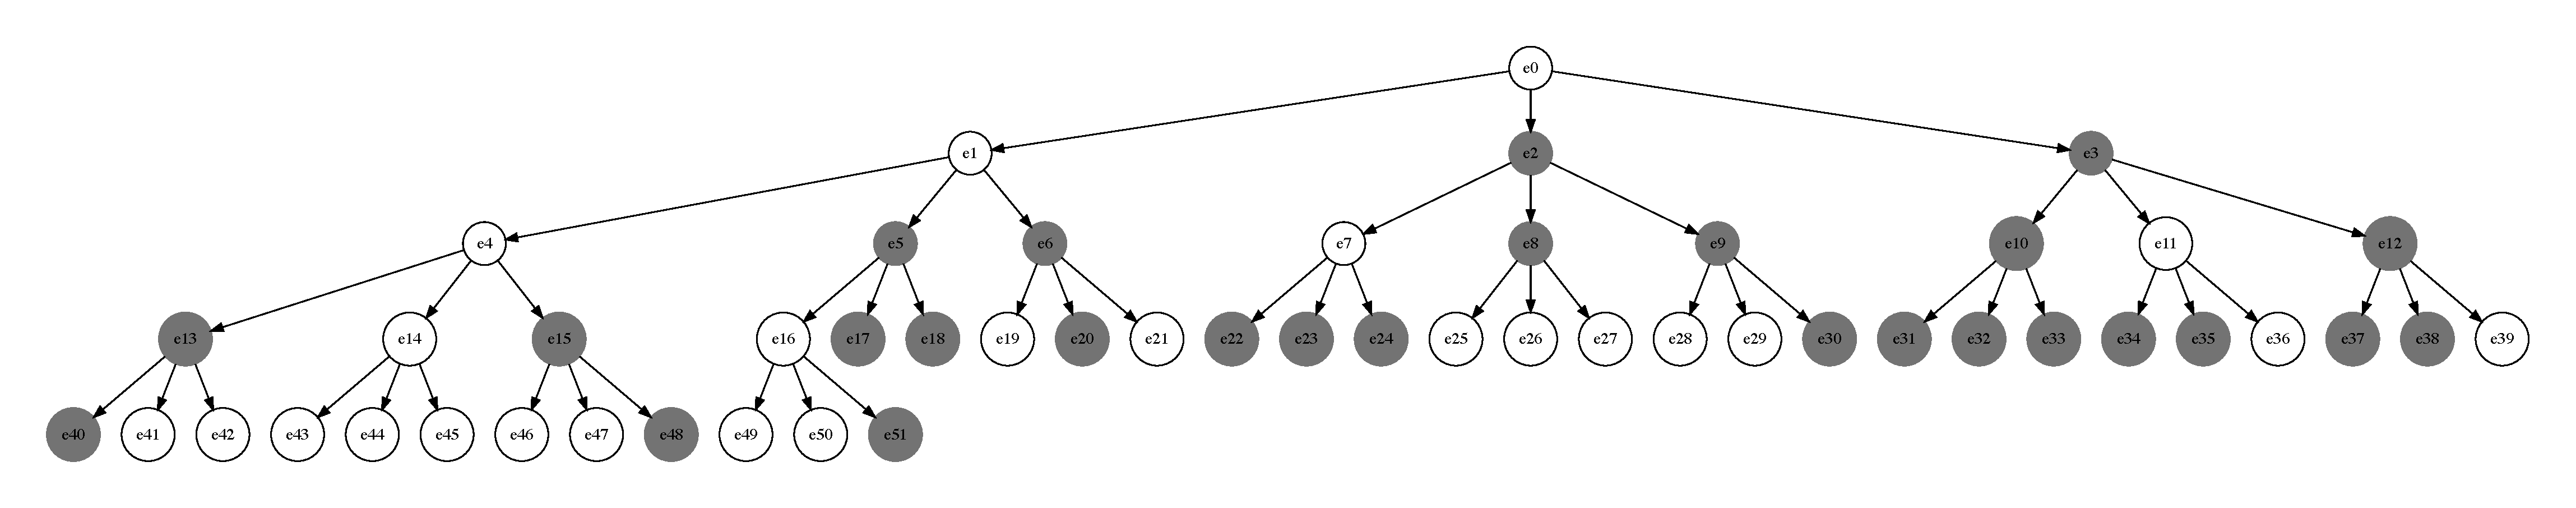
\includegraphics[width=\textwidth]{figs/Uni-hierachy.pdf}
  \end{minipage}
\end{figure}

For each employee, we use the generative model of Figure~\ref{fig:BN} to draw assignments for all the random variables. We assume that only $40\%$ of employees are qualified for promotion and regardless of their labels, employees submit only $60\%$ of their opinions. In addition, due to various personal and environmental factors, only $60\%$ of high quality employees perform well while $10\%$ of low quality employees also perform well regardless of their labels. Note that these numbers are not specific and just chosen for the framework to serve as a representative setting and a proof of concept. The conditional probability table for the opinion variable $O$ is parameterized by four values $(\theta_1, \theta_2, \theta_3, \theta_4)$ which together determine the degree of discrimination against the protected group. Since other parameters in the Bayesian network did not have a direct effect on the degree of discrimination, we fixed them to arbitrary values. 

The results presented in this section are based on an organization hierarchy  with $100$ employees where $k=5$. However, the results of the framework are not sensitive to the settings as we test the framework with various organization sizes ranging from $50$ to $500$ employees and various degree for $k$ ranging from $3$ to $10$. We generated seven datasets given the organization hierarchy using different values for the $\theta$ parameters: $(0.0,1.0,0.0,0.0)$, $(0.33,1.0,0.0,0.0)$, $(0.66,1.0,0.0,0.0)$, $(1.0,1.0,0.0,0.0)$, $(1.0,1.0,0.0,0.33)$, $(1.0,1.0,0.0,0.66)$, $(1.0,1.0,0.0,1.0)$. 
 
In the first three settings the discrimination originates from negative opinions towards qualified outgroup employees. The first setup is an extreme case where the opinion towards outgroup employees is always negative. The discrimination in the last three settings originates from positive opinions towards unqualified ingroup employees. The last setup is an extreme case where the opinion towards ingroup employees is always positive. The fourth setup represent unbiased opinions where employees are treated similarly based on their qualification. 

\paragraph{MAP Inference} We use the model presented in Table~\ref{tab:pslmodel} for MAP inference in PSL and FairPSL (recall that in FairPSL, the $\delta$-fairness constraints corresponding to one of the fairness measures are also added to the model). The observed atoms are $\textit{Manager(m,e)}$, $\textit{PositiveReview(e1,e2)}$ and labels of all employees. The truth values for all other atoms are obtained via MAP inference. We use the truth values obtained for the decision atoms $\textit{ToPromote(e)}$ to compute the fairness measures. We defined the discriminative pattern, and the protected and unprotected groups of this problem in Section~\ref{sec:formulation}.


\subsection{Evaluation results}

\begin{figure}
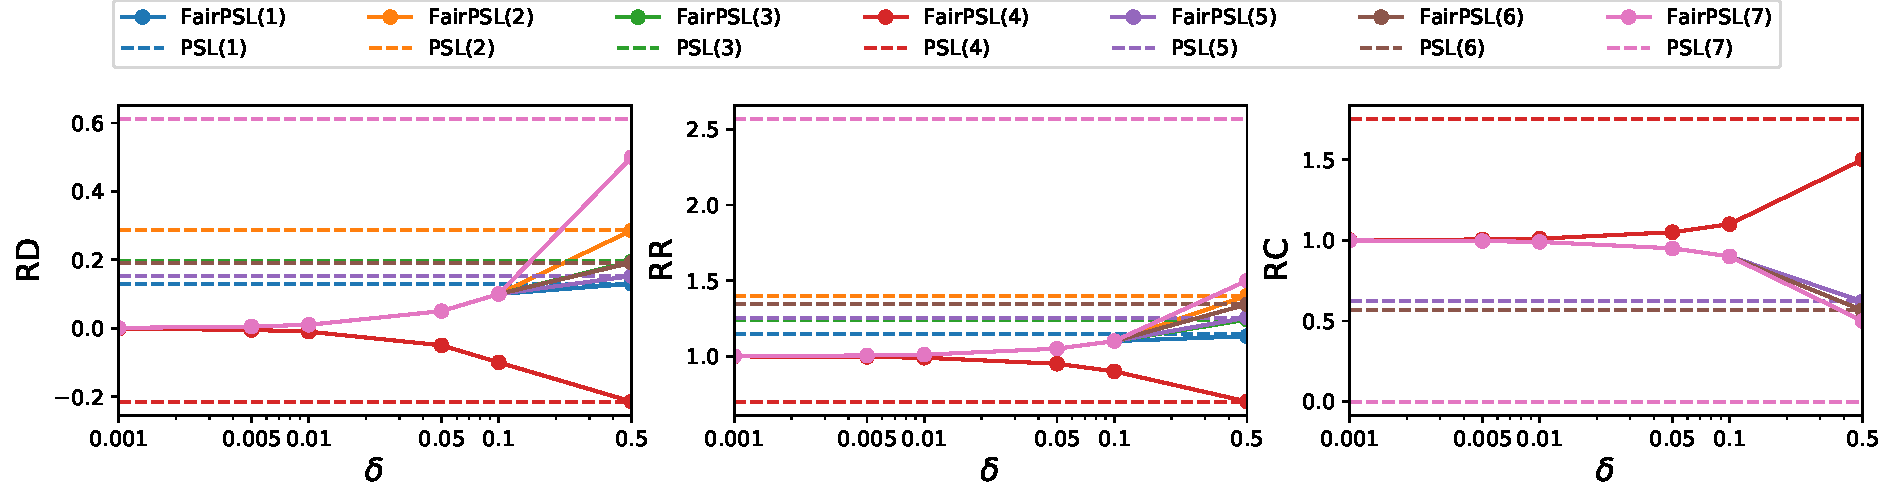
\includegraphics[width=1\linewidth]{figs/results_vis_uni_params.pdf}
\caption{\small Fairness score of predictions obtained by MAP inference of PSL and FairPSL, according to the fairness measures \emph{RD}, \emph{RR}, and \emph{RC}. The labels of datasets are mentioned with parenthesis next to the inference method. The FairPSL values of each measure are obtained by adding the $\delta$-fairness constraint of that measure.\label{fig:results}
}  
\end{figure}

To answer \textbf{Q1}, we run the MAP inference algorithm of PSL and FairPSL on seven synthetic datasets. 
We run the MAP inference of FairPSL multiple times on each dataset: For each of the three fairness measures, we add the corresponding $\delta$-fairness constraint with five thresholds $\{0.001, 0.005, 0.01, 0.05, 0.1, 0.5\}$.

Figure~\ref{fig:results} shows the fairness score of predictions in terms of the three fairness measures. As expected, tighter $\delta$-fairness constraints lead to better scores. Note that the best possible score according to RD is 0, as it computes a difference. Since RR and RC compute ratios, the best possible score according to these measures is 1. In our experiments, with any of these measures, taking $\delta = 0.001$ pushes the score of predictions to its limit.  

The $\delta$-fairness constraints modify the optimization problem of MAP inference by reducing the feasible region to solutions that conform with fairness guarantees. Research question \textbf{Q2} is concerned with the effect of this reduction on the accuracy of predictions. Note that decision quality is the same as the accuracy of predictions. To answer this question, we compare the inferred values for the decision atoms \textit{ToPromote(e)} against their actual values. These values are extracted from the known values of \textit{IsQualified(e)} according to rules 11 and 12 in Table~\ref{tab:pslmodel}. Figure~\ref{fig:accuracy} shows the area under the curve of the receiver operating characteristic~(AUC) of predicting the decision variable in three groups, namely the protected group, the unprotected group (i.e., promotion of the employees who have in-group managers), and all employees. By doing so, we make sure that our fairness constraints do not propagate bias towards either of the populations. Since the results of FairPSL with $\delta$-fairness constraints RR and RC are very similar to the results of RD, we only report the latter here.


\begin{figure}
    \centering
    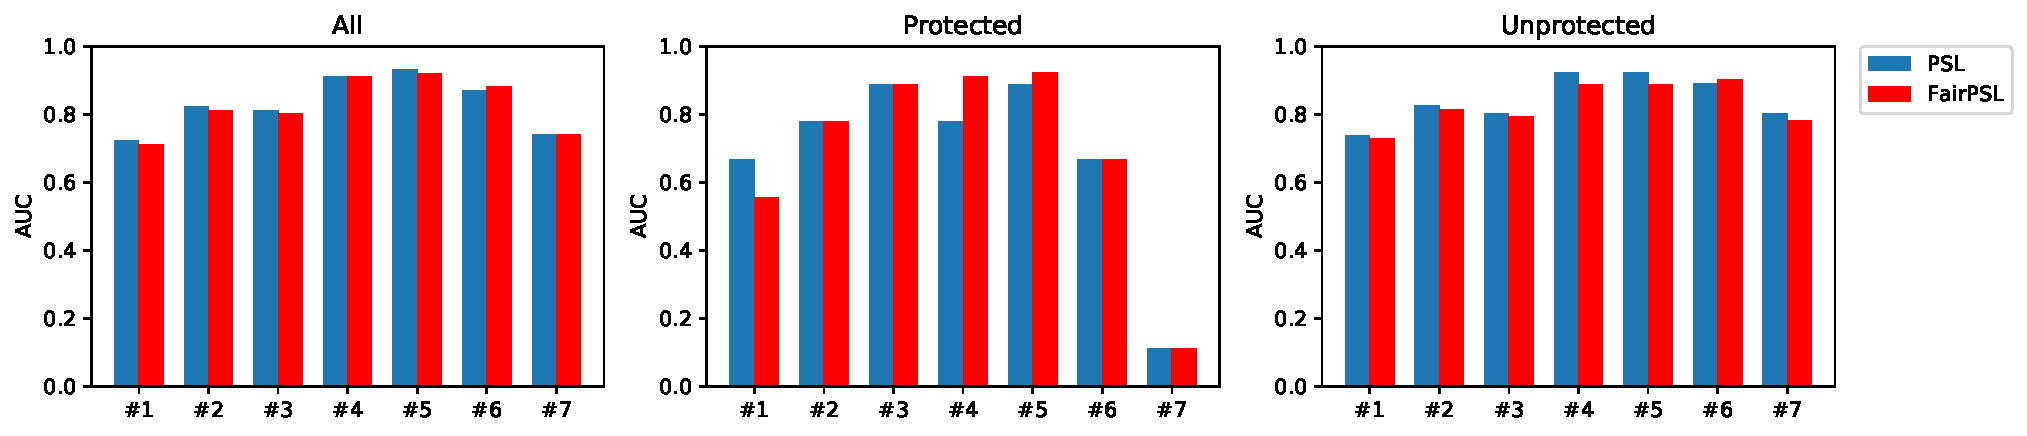
\includegraphics[width=\textwidth]{figs/roc.pdf}
    \caption{\small AUC score of predictions for truth values of unknown atoms \textit{ToPromote(e)} using MAP inference of PSL and FairPSL with $\delta$-fairness constraints $RD$ with $\delta=0.001$.}
    \label{fig:accuracy}
\end{figure}

According to Figure~\ref{fig:accuracy}, the results of both PSL and FairPSL in all seven datasets are close to each other. Note that although fairness may impose a cost in terms of overall accuracy, FairPSL often improves the accuracy of the protected class. Sometimes the overall predictions of FairPSL are even slightly better than PSL (e.g., dataset 6 and 7). As expected, the accuracy of the fourth setting where the opinions are unbiased are similar in both PSL and FairPSL. We observe that prediction of MAP inference for both FairPSL and PSL are similar, thus, in these settings at least, FairPSL guarantees fairness without hurting accuracy. Further investigation is required on the effect of the various ranges of discrimination (i.e., $\theta_1$, $\theta_2$, $\theta_3$, $\theta_4$) on the prediction results of FairPSL.



We also generate various types of organizations in which labels are not uniformly distributed, e.g., one population only occurs at the bottom levels of an organization. While we did not observe any differences in the behavior of our method with respect to accuracy and fairness measure, we found that the degree of discrimination is higher in such organizations. Further investigations on the structure of an organization on discrimination is an interesting direction for future research. 

\section{Conclusion and Future Directions}
\label{sec:conclusion}
Many applications of AI and machine learning affect peoples' lives in important ways. While there is a growing body of work on fairness in AI and ML, it assumes an individualistic notion of fairness.   In this paper, we have proposed a general framework for relational fairness which includes both a rich language for defining discrimination patterns and an efficient algorithm for performing inference subject to fairness constraints. We show our approach enforces fairness guarantees while preserving the accuracy of the predictions. 

There are many avenues for expanding on this work. For example, here we assumed that the discriminative pattern is given, however an automatic mechanism to extract discriminatory situations hidden in a large amount of decision records is an important and required task. Discrimination discovery has been studied for attribute-based fairness~\cite{pedreschi2013discovery}. An interesting next step is discrimination pattern discovery in relational data.

\section*{Acknowledgements}
This work is supported by the National Science Foundation under Grant Numbers CCF-1740850 and IIS-1703331. Golnoosh Farnadi and Behrouz Babaki are  supported by postdoctoral scholarships from IVADO through the Canada First Research Excellence Fund (CFREF) grant.

\begin{thebibliography}{10}
\itemsep=1pt 
\begin{small}

\bibitem{EUlaw}
European union legislation. (a) racial equality directive, 2000; (b) employment
  equality directive, 2000; (c) gender employment directive, 2006; (d) equal
  treatment directive (proposal), 2008.

\bibitem{UKlaw}
{UK} legislation. (a) sex discrimination act, 1975, (b) race relation act,
  1976.

\bibitem{USlaw}
United nations legislation. (a) universal declaration of human rights, 1948,
  (c) convention on the elimination of all forms of racial discrimination,
  1966, (d) convention on the elimination of all forms of discrimination
  against women, 1979.

\bibitem{alshukaili:iswc16}
Duhai Alshukaili, Alvaro A.~A. Fernandes, and Norman~W. Paton.
\newblock Structuring linked data search results using probabilistic soft
  logic.
\newblock In {\em International Semantic Web Conference {(1)}}, volume 9981 of
  {\em Lecture Notes in Computer Science}, pages 3--19, 2016.

\bibitem{bach:jmlr17}
Stephen~H. Bach, Matthias Broecheler, Bert Huang, and Lise Getoor.
\newblock Hinge-loss markov random fields and probabilistic soft logic.
\newblock {\em Journal of Machine Learning Research}, 18:109:1--109:67, 2017.

\bibitem{barocas2016big2}
Solon Barocas and Andrew~D Selbst.
\newblock Big data's disparate impact.
\newblock {\em California Law Review}, 104:671, 2016.

\bibitem{boyd2014networked}
Danah Boyd, Karen Levy, and Alice Marwick.
\newblock The networked nature of algorithmic discrimination.
\newblock In {\em Data and discrimination: Collected essays}, pages 53--57.
  2014.

\bibitem{brewer1979group}
Marilynn~B Brewer.
\newblock In-group bias in the minimal intergroup situation: A
  cognitive-motivational analysis.
\newblock {\em Psychological bulletin}, 86(2):307, 1979.

\bibitem{brewer2007social}
Marilynn~B Brewer.
\newblock The social psychology of intergroup relations: Social categorization,
  ingroup bias, and outgroup prejudice.
\newblock {\em Social Psychology: Handbook of Basic Principles}, 2007.

\bibitem{chouldechova2017fair2}
Alexandra Chouldechova.
\newblock Fair prediction with disparate impact: {A} study of bias in
  recidivism prediction instruments.
\newblock {\em CoRR}, abs/1703.00056, 2017.

\bibitem{dwork2012fairness3}
Cynthia Dwork, Moritz Hardt, Toniann Pitassi, Omer Reingold, and Richard~S.
  Zemel.
\newblock Fairness through awareness.
\newblock In {\em {ITCS}}, pages 214--226. {ACM}, 2012.

\bibitem{ebrahimi:emnlp16}
Javid Ebrahimi, Dejing Dou, and Daniel Lowd.
\newblock Weakly supervised tweet stance classification by relational
  bootstrapping.
\newblock In {\em {EMNLP}}, pages 1012--1017. The Association for Computational
  Linguistics, 2016.

\bibitem{farnadi2018fairness}
Golnoosh Farnadi, Behrouz Babaki, and Lise Getoor.
\newblock Fairness in relational domains.
\newblock In {\em AAAI/ACM Conference on AI, Ethics, and Society (AIES)}, pages
  108--114. ACM, 2018.

\bibitem{feldman2015certifying2}
Michael Feldman, Sorelle~A. Friedler, John Moeller, Carlos Scheidegger, and
  Suresh Venkatasubramanian.
\newblock Certifying and removing disparate impact.
\newblock In {\em {KDD}}, pages 259--268. {ACM}, 2015.

\bibitem{getoor2007introduction}
Lise Getoor and Ben Taskar.
\newblock {\em {Introduction to Statistical Relational Learning}}.
\newblock MIT press Cambridge, 2007.

\bibitem{hardt2016equality3}
Moritz Hardt, Eric Price, and Nati Srebro.
\newblock Equality of opportunity in supervised learning.
\newblock In {\em {NIPS}}, pages 3315--3323, 2016.

\bibitem{kamishima2011fairness}
Toshihiro Kamishima, Shotaro Akaho, and Jun Sakuma.
\newblock Fairness-aware learning through regularization approach.
\newblock In {\em ICDMW}, pages 643--650. {IEEE} Computer Society, 2011.

\bibitem{kouki:recsys15}
Pigi Kouki, Shobeir Fakhraei, James~R. Foulds, Magdalini Eirinaki, and Lise
  Getoor.
\newblock Hyper: {A} flexible and extensible probabilistic framework for hybrid
  recommender systems.
\newblock In {\em RecSys}, pages 99--106. {ACM}, 2015.

\bibitem{counterfactualfairness}
Matt~J. Kusner, Joshua~R. Loftus, Chris Russell, and Ricardo Silva.
\newblock Counterfactual fairness.
\newblock In {\em {NIPS}}, pages 4069--4079, 2017.

\bibitem{Pedreschi:2012}
Dino Pedreschi, Salvatore Ruggieri, and Franco Turini.
\newblock A study of top-k measures for discrimination discovery.
\newblock In {\em {SAC}}, pages 126--131. {ACM}, 2012.

\bibitem{pedreschi2013discovery}
Dino Pedreschi, Salvatore Ruggieri, and Franco Turini.
\newblock The discovery of discrimination.
\newblock In {\em Discrimination and Privacy in the Information Society},
  volume~3 of {\em Studies in Applied Philosophy, Epistemology and Rational
  Ethics}, pages 91--108. Springer, 2013.

\bibitem{ridgeway2004unpacking}
Cecilia~L Ridgeway and Shelley~J Correll.
\newblock Unpacking the gender system: A theoretical perspective on gender
  beliefs and social relations.
\newblock {\em Gender \& society}, 18(4):510--531, 2004.

\bibitem{sridhar:bioinformatics16}
Dhanya Sridhar, Shobeir Fakhraei, and Lise Getoor.
\newblock A probabilistic approach for collective similarity-based drug-drug
  interaction prediction.
\newblock {\em Bioinformatics}, 32(20):3175--3182, 2016.

\bibitem{verma2018fairness2}
Sahil Verma and Julia Rubin.
\newblock Fairness definitions explained.
\newblock In {\em 2018 IEEE/ACM International Workshop on Software Fairness
  (FairWare)}, pages 1--7. IEEE, 2018.

\bibitem{west2014exploiting}
Robert West, Hristo~S. Paskov, Jure Leskovec, and Christopher Potts.
\newblock Exploiting social network structure for person-to-person sentiment
  analysis.
\newblock {\em {TACL}}, 2:297--310, 2014.

\bibitem{zafar2017parity}
Muhammad~Bilal Zafar, Isabel Valera, Manuel Gomez{-}Rodriguez, Krishna~P.
  Gummadi, and Adrian Weller.
\newblock From parity to preference-based notions of fairness in
  classification.
\newblock In {\em {NIPS}}, pages 228--238, 2017.

\bibitem{zemel2013learning}
Richard~S. Zemel, Yu~Wu, Kevin Swersky, Toniann Pitassi, and Cynthia Dwork.
\newblock Learning fair representations.
\newblock In {\em {ICML} {(3)}}, volume~28 of {\em {JMLR} Workshop and
  Conference Proceedings}, pages 325--333. JMLR.org, 2013.

\end{small}
\end{thebibliography}

\end{document}

\end{article}



\end{articlesection}

%\begin{newssection}{TCDE Election}
%
% there will be other letters- and a blank page will appear in your document
% but the special issue part will be fine
%
%\begin{news}{Letter from the Editor-in-Chief}
%{David Lomet}{Microsoft Corporation}
%\documentclass[11pt]{article} 

\usepackage{deauthor,times,graphicx}
%\usepackage{url}
\usepackage{hyperref}

\begin{document}

\subsection*{ICDE 2018}

Repeating my comment from the last issue-

The IEEE International Conference on Data Engineering will be held in April 14-19, 2018 in Paris, France.  This is the flagship conference of the Computer Society's Technical Committee on Data Engineering.  It is a great conference, at a great location.  What could possibly be better than April in Paris at ICDE!  I am attending and hope to see you there.

\subsection*{About the Bulletin}

This March current issue marks the end of editorial tenure for the Bulletin's current set of editors.  So it is once again time for me to pat myself on the back.  This current set, Tim Kraska, Tova Milo, and Haixun Wang, continue my outstanding success (he says modestly) in finding and choosing great editors.  All three have done truly fine jobs at producing issues that bring to our readers surveys of the latest work in very current areas. The success of the Bulletin depends on great issue editors.  I want to thank Tim, Tova, and Haixun for being exactly that with the fine jobs that they have done.  There was unexpected ``scrambling" over the past two years, so I want to thank them also for their flexibility in coping with this.  


\subsection*{The Current Issue}

Don't you get tired of someone shouting ``FAKE NEWS!".  Or perhaps even worse, being exposed to fake news before it has been labeled as such?  Our political conversations seem increasingly to include many variations of ``fake news" and discussions about which news is fake.  ``Sad." So where am I going with this?

The database world has been working on a key aspect of this problem for many years.  The technical area is called ``data provenance".  And it addresses the problem of where information comes from and how it impacts the subsequent processing of data and the reported results.  The June, 2010 issue was the last one on provenance.  And seven years is a long time in an active technical area, especially an area as important as this.

The current issue is focused on the applications of provenance.  Without delving into the current political scene, a reader will clearly see how extensively provenance management can be used.  As we gain more insight into its application scenarios, we also gain more insight into how to manage provenance.  This symbiotic relationship is driving the field forward.   Tova Milo, our Bulletin editor for the issue, has done an excellent job in bringing the issue together, making it a great place to learn about and track progress in the field.  The result is an issue well worth reading.



\end{document}



%\end{news}
%
%\newpage
%
%% your introductory letter goes here
%
%\begin{news}{Letter from the Special Issue Editor}
%{Joseph E. Gonzalez}{University of California at Berkeley\\ Berkeley, CA}
%\graphicspath{{letters/}}
%\documentclass[11pt]{article} 

\usepackage{deauthor,times,graphicx}
%\usepackage{url}
\usepackage{hyperref}



\begin{document}

Machine learning is rapidly maturing into an engineering discipline at the center of a growing range of applications.
This widespread adoption of machine learning techniques presents new challenges around the management of the data, code, models, and their relationship throughout the machine learning life-cycle.
In this special issue, 
% of the Data Engineering Bulletin 
we have solicited work from both academic and industrial leaders 
% in the data engineering community that 
who are exploring how data engineering techniques can be used to address the challenges of the machine learning life-cycle.




\begin{figure}[h]
\centering
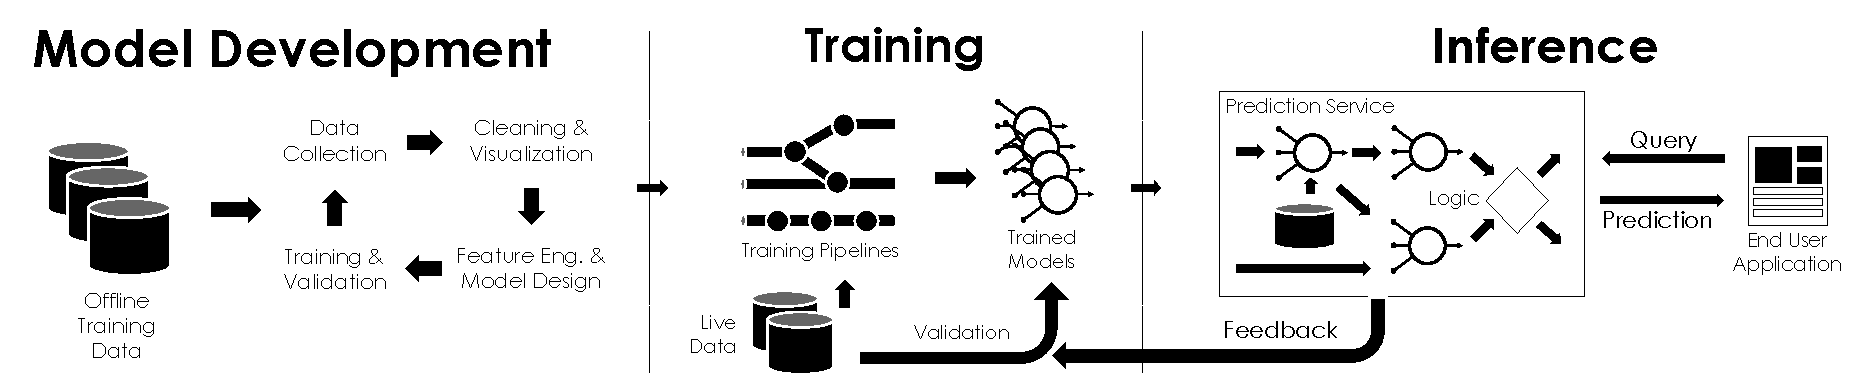
\includegraphics[width=\textwidth]{letters/pipeline.pdf}
\caption{\small \textbf{Machine Learning Life-cycle.} A simplified depiction of the key stages of a machine learning application.}
\label{fig:mllc}
\end{figure}


The machine learning life-cycle (Fig.~\ref{fig:mllc}) spans not only the model development but also production training and inference.
Each stage demands different skills (e.g., neural network design, data management, and cluster management) and imposes different requirements on the underlying systems.
Yet there is an overwhelming need for unifying design principles and technologies to address pervasive problems including feature management, data provenance, pipeline reproducibility, low-latency serving, and prediction monitoring just to name a few.


There has been a flurry of recent progress in systems to aid in managing the machine learning life-cycle.  
Large industrial projects like 
FB Learner Flow 
% \href{https://code.fb.com/core-data/introducing-fblearner-flow-facebook-s-ai-backbone/}{FB Learner Flow}
from Facebook, 
Michelangelo 
% \href{https://eng.uber.com/michelangelo/}{Michelangelo} 
from Uber, and 
TFX 
% \href{https://www.tensorflow.org/tfx/}{TFX} 
from Google have received considerable recent attention.  
In this issue, we have solicited papers from several recent industrial and academic projects that have received slightly less attention.


The first paper provides an overview of several real-world use cases and then outlines the key conceptual, data management, and engineering challenges faced in production machine learning systems.
% Rather than advocating a single system, this work describes some design principles that can inform potential solutions.
The second and third papers explores the challenges of model management and provenance across the machine learning life-cycle.
They motivate the need for systems to track models and their meta-data to improve reproducibility, collaboration, and governance. 
% expands upon the machine learning life-cycle 
% to include: data preparation, feature engineering, model training, deployment, and maintenance
% and explores the challenges of model 
The second paper introduces, ModelDB, an open-source system for model management and describe some of the functionality and design decisions. 
The third paper describes a related system, ProvDB, that uses a graph data model to capture and query fine-grained versioned lineage of data, scripts, and artifacts throughout the data analysis process.
The fourth paper describes, MLFlow, a new open-source system to address the challenges of experimentation, reproducibility, and deployment. 
This work leverages containerization to capture the model development environment and a simple tracking API to enable experiment tracking.
% The extensible model containerization enables model developers to more easily collaborate around modeling environments and then deploy model containers.
The fifth paper focuses on inference and explores the challenges and opportunities of serving white-box prediction pipelines.  
Finally, we solicited a summary of the recent Common Modeling Infrastructure (CMI) workshop at KDD 2018, which provides a summary of the keynotes and contributed talks.

The work covered here is only a small sample of the emerging space of machine learning life-cycle management systems. 
We anticipate that this will be a growing area of interest for the data engineering community.


% In contrast to the containerization of pipelines in MLFlow, the Microsoft team leverage knowledge about the internal of the prediction pipeline to more efficient serve predictions. 



\end{document}



%\end{news}


%\end{newssection}

%\begin{newssection}{TCDE Election}

% there will be other letters- and a blank page will appear in your document
% but the special issue part will be fine

%\begin{news}{Letter from the Editor-in-Chief}
%{David Lomet}{Microsoft Corporation}
%\documentclass[11pt]{article} 

\usepackage{deauthor,times,graphicx}
%\usepackage{url}
\usepackage{hyperref}

\begin{document}

\subsection*{ICDE 2018}

Repeating my comment from the last issue-

The IEEE International Conference on Data Engineering will be held in April 14-19, 2018 in Paris, France.  This is the flagship conference of the Computer Society's Technical Committee on Data Engineering.  It is a great conference, at a great location.  What could possibly be better than April in Paris at ICDE!  I am attending and hope to see you there.

\subsection*{About the Bulletin}

This March current issue marks the end of editorial tenure for the Bulletin's current set of editors.  So it is once again time for me to pat myself on the back.  This current set, Tim Kraska, Tova Milo, and Haixun Wang, continue my outstanding success (he says modestly) in finding and choosing great editors.  All three have done truly fine jobs at producing issues that bring to our readers surveys of the latest work in very current areas. The success of the Bulletin depends on great issue editors.  I want to thank Tim, Tova, and Haixun for being exactly that with the fine jobs that they have done.  There was unexpected ``scrambling" over the past two years, so I want to thank them also for their flexibility in coping with this.  


\subsection*{The Current Issue}

Don't you get tired of someone shouting ``FAKE NEWS!".  Or perhaps even worse, being exposed to fake news before it has been labeled as such?  Our political conversations seem increasingly to include many variations of ``fake news" and discussions about which news is fake.  ``Sad." So where am I going with this?

The database world has been working on a key aspect of this problem for many years.  The technical area is called ``data provenance".  And it addresses the problem of where information comes from and how it impacts the subsequent processing of data and the reported results.  The June, 2010 issue was the last one on provenance.  And seven years is a long time in an active technical area, especially an area as important as this.

The current issue is focused on the applications of provenance.  Without delving into the current political scene, a reader will clearly see how extensively provenance management can be used.  As we gain more insight into its application scenarios, we also gain more insight into how to manage provenance.  This symbiotic relationship is driving the field forward.   Tova Milo, our Bulletin editor for the issue, has done an excellent job in bringing the issue together, making it a great place to learn about and track progress in the field.  The result is an issue well worth reading.



\end{document}



%\end{news}
%
%\newpage
%
%% your introductory letter goes here
%
%\begin{news}{Letter from the Special Issue Editor}
%{Joseph E. Gonzalez}{University of California at Berkeley\\ Berkeley, CA}
%\documentclass[11pt]{article} 

\usepackage{deauthor,times,graphicx}
%\usepackage{url}
\usepackage{hyperref}



\begin{document}

Machine learning is rapidly maturing into an engineering discipline at the center of a growing range of applications.
This widespread adoption of machine learning techniques presents new challenges around the management of the data, code, models, and their relationship throughout the machine learning life-cycle.
In this special issue, 
% of the Data Engineering Bulletin 
we have solicited work from both academic and industrial leaders 
% in the data engineering community that 
who are exploring how data engineering techniques can be used to address the challenges of the machine learning life-cycle.




\begin{figure}[h]
\centering
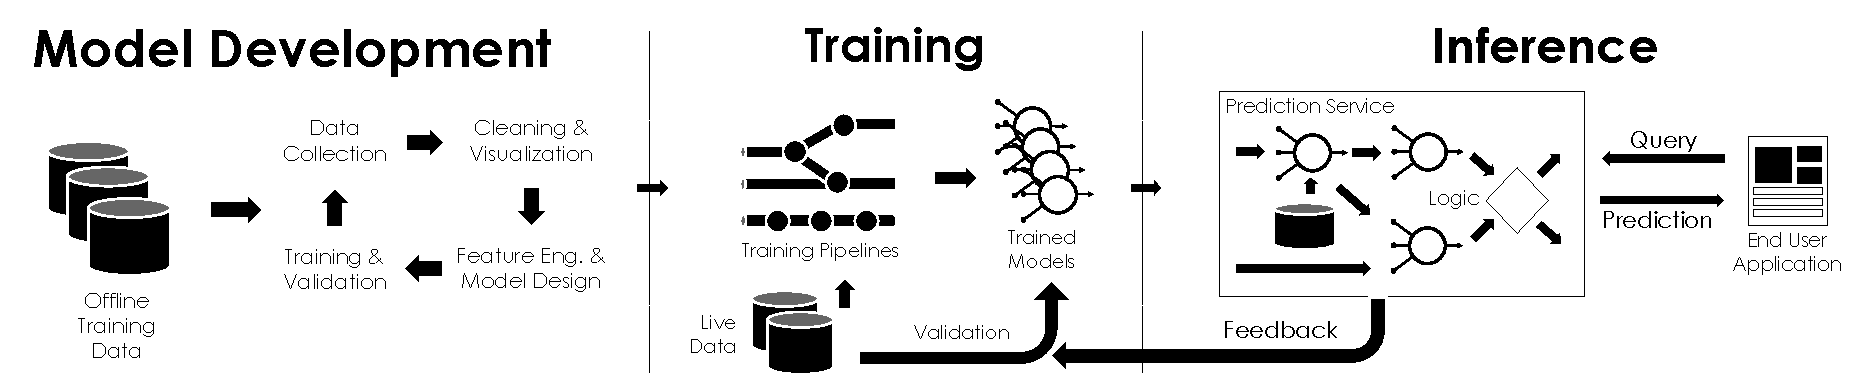
\includegraphics[width=\textwidth]{letters/pipeline.pdf}
\caption{\small \textbf{Machine Learning Life-cycle.} A simplified depiction of the key stages of a machine learning application.}
\label{fig:mllc}
\end{figure}


The machine learning life-cycle (Fig.~\ref{fig:mllc}) spans not only the model development but also production training and inference.
Each stage demands different skills (e.g., neural network design, data management, and cluster management) and imposes different requirements on the underlying systems.
Yet there is an overwhelming need for unifying design principles and technologies to address pervasive problems including feature management, data provenance, pipeline reproducibility, low-latency serving, and prediction monitoring just to name a few.


There has been a flurry of recent progress in systems to aid in managing the machine learning life-cycle.  
Large industrial projects like 
FB Learner Flow 
% \href{https://code.fb.com/core-data/introducing-fblearner-flow-facebook-s-ai-backbone/}{FB Learner Flow}
from Facebook, 
Michelangelo 
% \href{https://eng.uber.com/michelangelo/}{Michelangelo} 
from Uber, and 
TFX 
% \href{https://www.tensorflow.org/tfx/}{TFX} 
from Google have received considerable recent attention.  
In this issue, we have solicited papers from several recent industrial and academic projects that have received slightly less attention.


The first paper provides an overview of several real-world use cases and then outlines the key conceptual, data management, and engineering challenges faced in production machine learning systems.
% Rather than advocating a single system, this work describes some design principles that can inform potential solutions.
The second and third papers explores the challenges of model management and provenance across the machine learning life-cycle.
They motivate the need for systems to track models and their meta-data to improve reproducibility, collaboration, and governance. 
% expands upon the machine learning life-cycle 
% to include: data preparation, feature engineering, model training, deployment, and maintenance
% and explores the challenges of model 
The second paper introduces, ModelDB, an open-source system for model management and describe some of the functionality and design decisions. 
The third paper describes a related system, ProvDB, that uses a graph data model to capture and query fine-grained versioned lineage of data, scripts, and artifacts throughout the data analysis process.
The fourth paper describes, MLFlow, a new open-source system to address the challenges of experimentation, reproducibility, and deployment. 
This work leverages containerization to capture the model development environment and a simple tracking API to enable experiment tracking.
% The extensible model containerization enables model developers to more easily collaborate around modeling environments and then deploy model containers.
The fifth paper focuses on inference and explores the challenges and opportunities of serving white-box prediction pipelines.  
Finally, we solicited a summary of the recent Common Modeling Infrastructure (CMI) workshop at KDD 2018, which provides a summary of the keynotes and contributed talks.

The work covered here is only a small sample of the emerging space of machine learning life-cycle management systems. 
We anticipate that this will be a growing area of interest for the data engineering community.


% In contrast to the containerization of pipelines in MLFlow, the Microsoft team leverage knowledge about the internal of the prediction pipeline to more efficient serve predictions. 



\end{document}



%\end{news}

%\end{newssection}



\begin{callsection}
%  This section will be empty for your version
%
%  Calls for papers section.  Use the callsection environment.
%  Each call for papers is contained in an call environment, where the single 
%  required options to \begin{call} is the name of the conference.
%
\begin{call}{ICDE 2019 Conference}
\centerline{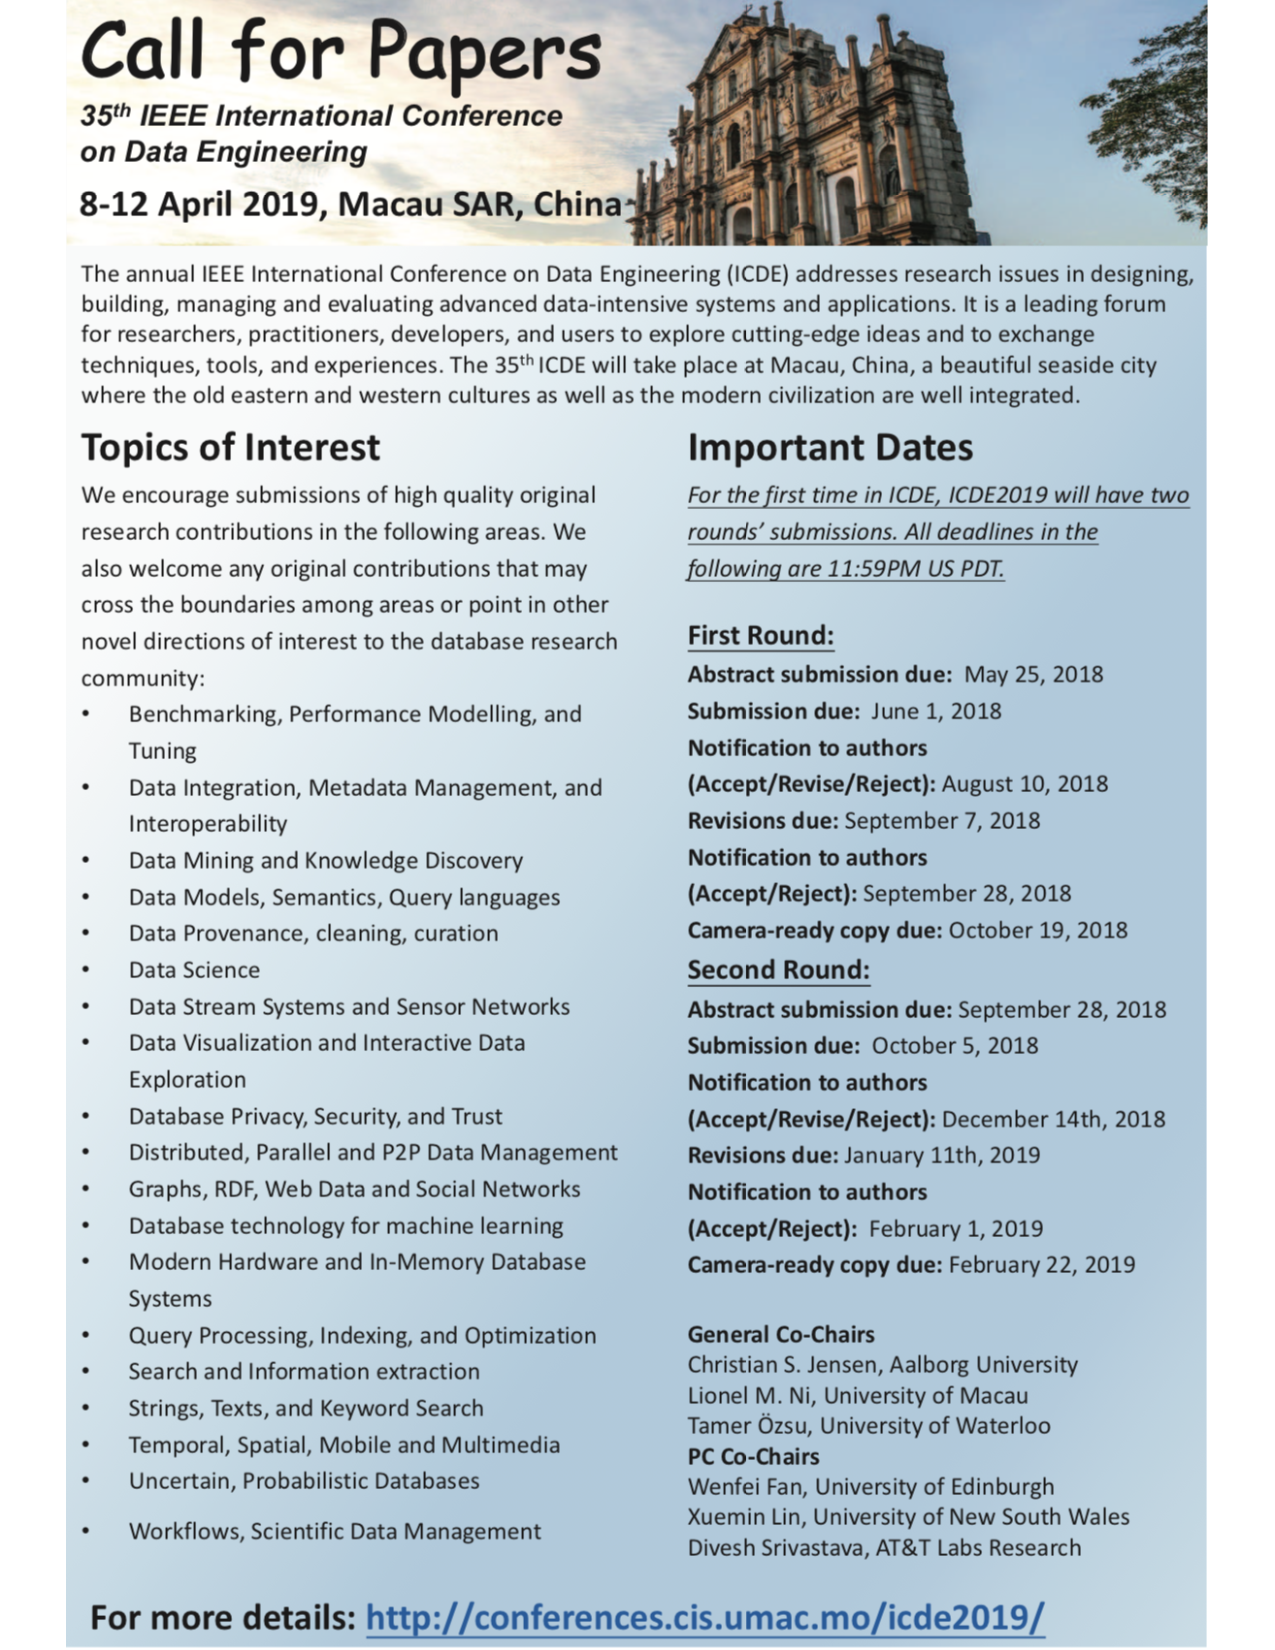
\includegraphics[width=\textwidth, bb= 0 0 610 790] {calls/icde19.pdf}} 
%\centerline{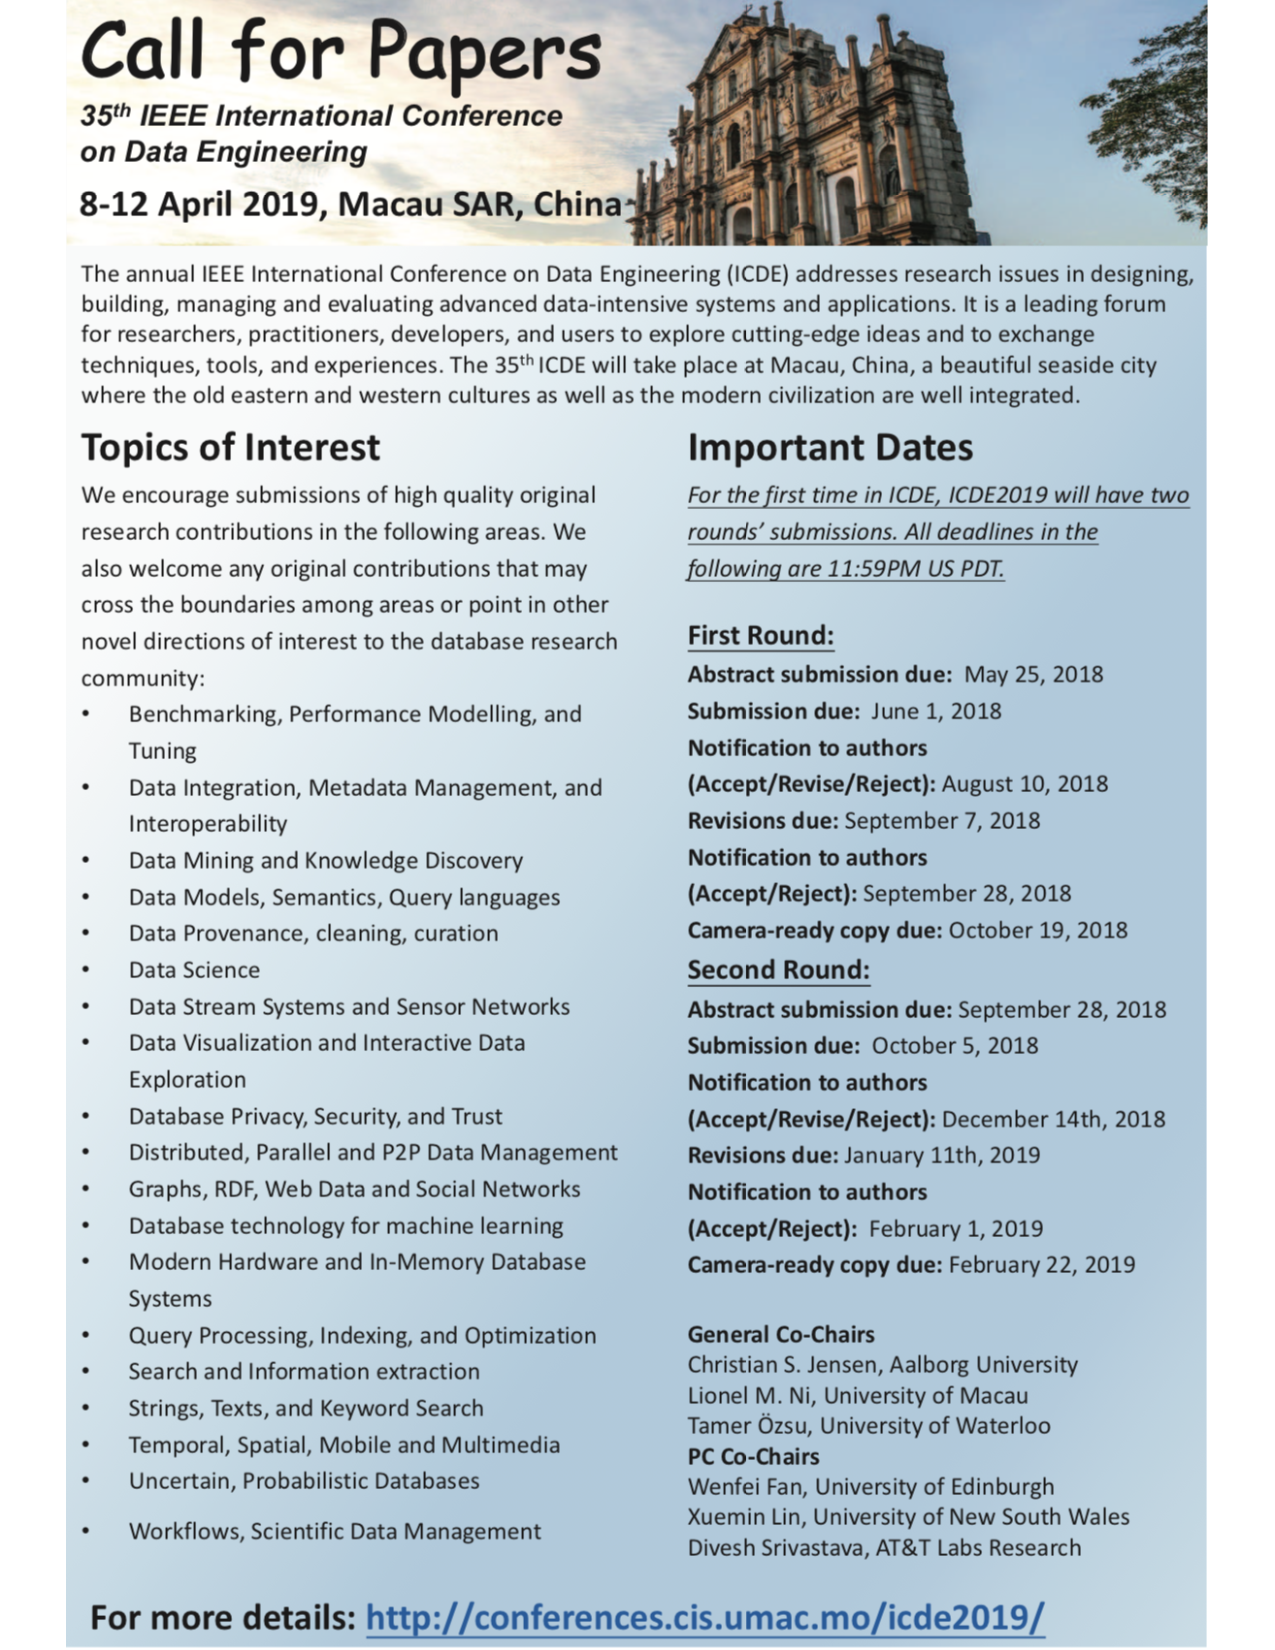
\includegraphics[width=\textwidth, bb= 0 0 590 760] {calls/icde19.pdf}}
\end{call}
\begin{call}{TCDE Membership Form}
%\centerline{\includegraphics[width=\textwidth, bb= 0 0 610 790]
\centerline{
\includegraphics[width=\textwidth, bb= 0 0 590 760] {calls/tcde.pdf}}
\end{call}
\end{callsection}

\end{bulletin}
\end{document}
